\documentclass[11pt]{article}
\usepackage[textwidth=420pt,textheight=650pt,headheight=13.6pt,nofoot,includehead]{geometry}
\usepackage{bm}
\usepackage{amsmath}
\usepackage{amssymb}
\usepackage{hyperref}
\usepackage{relsize}
\usepackage{xspace}
\usepackage{multicol}
\usepackage{nomencl}
\usepackage{titlesec}
\usepackage{titletoc}
\usepackage[bottom]{footmisc}
\usepackage{makeidx}
\usepackage{charter}
\usepackage{textfit}
\usepackage[numbers,sort&compress]{natbib}
\usepackage{hypernat}
\usepackage{fancyhdr}
\usepackage{fancyvrb}
\usepackage{bbold}
\usepackage[usenames]{color}
\usepackage{caption}
\renewcommand\captionlabelfont{\footnotesize\upshape\bfseries}
\renewcommand\captionfont{\footnotesize}
\makeindex
\usepackage{tableaux}

\newcommand{\dcite}[1]{{\citeauthor{#1}~\cite{#1}}}
\newcommand{\ddcite}[2]{{\citeauthor{#1}~\cite{#1,#2}}}
\setlength{\skip\footins}{15pt plus 4pt minus 2 pt}

\DeclareMathOperator{\sgn}{sgn}

% Screen environment, for display of verbatim material.

\makeatletter
\newcommand{\kcomment}[2]{{\bf [#1: #2]}}
\newcommand{\bfcomment}[2]{{\bf [#1: #2]}}
\newcommand{\outdated}{{\bfseries (documentation no longer correct!)}}
\fvset{frame=lines,framerule=0.1pt,framesep=6pt,numbers=none,xleftmargin=5ex,fontfamily=tt,fontsize=\small}
\newenvironment{screen}[1]{\hilitelines(#1)\Verbatim}{\endVerbatim}
\makeatother

\newif\ifhilite
\def\hilitelines(#1){%
  \def\FancyVerbFormatLine##1{%
    \def\fancylineinput{##1}%
    \hilitefalse
    \splitfirst #1,\relax,%
    \ifhilite\else
      \fancylineinput
    \fi}}

\def\splitfirst#1,{%
  \ifx\relax#1\empty\else
    \hiliteline{#1}{\fancylineinput}\expandafter\splitfirst
  \fi}

\def\hiliteline#1#2{%
    \ifhilite\else
      \ifnum\value{FancyVerbLine} = #1
      \llap{{\smaller\smaller \raisebox{.8ex}{$\vartriangleright$}}\,\,\,}%
      \fi
    \fi}

%        \colourcmd{#2}\hilitetrue
%\def\colourcmd{\colorbox{red}} 

% List layout.

\makenomenclature
%glossary
\setlength{\nomitemsep}{-\parsep}
%\renewcommand{\nomname}{\hspace{-3mm}\raisebox{3.2mm}{\hbox{\normalsize\it %
%      List of algorithms and properties:}}\vspace{-7mm}}
\renewcommand{\nomname}{\vspace{-17mm}}
\renewcommand{\nomlabel}[1]{{\tt \def\cdbat{@}\def\cdbcc{::}\def\cdbbs{$\backslash$}#1}\hfill}
\renewcommand{\pagedeclaration}[1]{#1~~~}
\renewcommand\descriptionlabel[1]{\hbox to \textwidth{\quad\quad\bf {#1}\hfill}}
\newcommand{\cdb}{{cadabra}\xspace}
\newcommand{\Cdb}{{Cadabra}\xspace}
\newcommand{\Cpp}{\leavevmode\rm{\hbox{C\hskip -0.1ex\raise 0.5ex\hbox{\tiny ++}}}\xspace}

% Three macros to declare the main usage of a command, property or
% member function (to appear in the table of contents of the module 
% section), and commands to use for every subsequent use in the
% text (which may at some stage end up in the index at the end).
\newcommand{\cdbcommand}[2]{\nomenclature{\cdbat#1}{\hfill\nomrefpage}{\tt @#1}}
\newcommand{\subscommand}[1]{{\tt @#1}}
\newcommand{\cdbprop}[2]{\nomenclature{\cdbcc#1}{\hfill\nomrefpage}{\tt ::#1}}

\newenvironment{props}{\par\noindent{\bf properties:}\description}{\enddescription}
\newenvironment{algs}{\par\noindent{\bf algorithms:}\description}{\enddescription}
\newenvironment{reserved}{\par\noindent\description}{\enddescription}

%\newenvironment{props}{\par\noindent{\bf properties:}\\[1ex]}{\bigskip\par}
%\newenvironment{algs}{\par\noindent{\bf algorithms:}\\[1ex]}{\bigskip\par}

\newcommand{\cdbalgorithm}[2]{\nomenclature{\cdbat#1}{\hfill\nomrefpage}\item[{\tt @#1}]}
\newcommand{\cdbproperty}[2]{\nomenclature{\cdbcc#1}{\hfill\nomrefpage}\item[{\tt ::#1}\if!#2!\else(#2)\fi]}
\newcommand{\cdbreserved}[2]{\nomenclature{\cdbbs#1}{\hfill\nomrefpage}\item[{\tt $\backslash$#1}\if!#2!\else\{#2\}\fi]}

%\newcommand{\cdbalgorithm}[2]{\nomenclature{\cdbat#1}{\hfill\refpage}\noindent{\tt @#1}\\}
%\newcommand{\cdbproperty}[2]{\nomenclature{\cdbcc#1}{\hfill\refpage}\noindent{\tt ::#1}\if#2{}\else(#2)\fi}

\newcommand{\cdbseealgo}[1]{}
\newcommand{\cdbseeprop}[1]{}
\newcommand{\subsprop}[1]{{\tt #1}}
\newcommand{\cdbclass}[1]{{\tt #1}}
\newcommand{\cdbfile}[1]{{\tt #1}}
\newcommand{\member}[1]{{\tt #1}}
\newcommand{\subsmember}[1]{{\tt #1}}
\newcommand{\deprecated}{\marginpar{{\bf\smaller deprecated}}}

\newcommand{\inertcommand}[1]{{\tt @@#1}}
\newcommand{\texcommand}[1]{{\tt $\backslash$#1}}
\newcommand{\ctri}{{\smaller\smaller$\blacktriangleright$}}
\newcommand{\boolargs}{{\it true\/}$|${\it false\/}}
\newcommand{\listargs}{{\it expression list\/}}

\numberwithin{equation}{section}

\def\mystrut{\vbox to 8.5pt{}\vtop to 3.5pt{}}
\def\V{\hskip10pt\vrule\hskip10pt}
\def\T{\hskip10pt\vrule\vrule height2.5pt depth -2.1pt width 10pt}
\def\L{\hskip10pt\vrule height 8.5pt depth -2.1pt
       \vrule height2.5pt depth -2.1pt width 10pt}
\def\N{\hskip10pt\phantom{\vrule}\hskip10pt}
\def\hw{\hskip-1000pt plus 1fil}

% Courtesy of Donald Arsenau.
\makeatletter
\newenvironment{descerate}
  {\enumerate
   \@noitemargtrue \let\@noitemargfalse\relax
   \renewcommand\makelabel[1]{%
     \hspace\labelwidth
     \llap{\@itemlabel}%
     \hspace\labelsep
     \textbf{##1}%
   }%
  }%
  {\endenumerate}
\makeatother
%\renewcommand{\contentsname}{\vspace{-3ex}}


% Page layout style
%
\pagestyle{fancy}
\renewcommand{\sectionmark}[1]{\markboth{{\it\small #1}}{}}%
\renewcommand{\subsectionmark}[1]{\markboth{{\it\small \thesubsection.~#1}}{}}%
\fancyhf{}%
\fancyhead[L]{\leftmark\hspace{3cm}}
\fancyhead[R]{\thepage}%
\renewcommand{\headrulewidth}{.1pt}
\renewcommand{\footrulewidth}{0pt}
\fancypagestyle{plain}{%
 \fancyhead{}
 }


%\newcommand{\sectionformat}[1]{\colorbox[rgb]{.84,.84,.95}{$\vcenter to 2.5ex{\vspace{-.45ex}\hbox
%	 to 444pt{\bfseries\textcolor[rgb]{0,0,0}{\Huge\bfseries \hspace{3mm}#1\strut\hfill}}}$}}
%\newcommand{\subsectionformat}[1]{\colorbox[rgb]{.9,.9,.98}{$\vcenter to 1.5ex{\hbox
%	 to 444pt{\bfseries\textcolor[rgb]{0,0,0}{\large\bfseries \hspace{3mm}\thesubsection~~#1\strut\hfill}}}$}}

\newcommand{\sectionformat}[1]{\Huge\bfseries \hspace{3mm}#1}
\newcommand{\subsectionformat}[1]{\large\bfseries \hspace{3mm}\thesubsection~~#1}

% \titlecontents{section}[0pt]{\addvspace{1pc}\itshape}%
%    {\contentsmargin{0pt}\bfseries%
%     \makebox[0pt][r]{\large\thecontentslabel\enspace}\large}%
%    {\contentsmargin{0pt}\large}
%    {\quad\thepage}[\addvspace{.5pc}]
\renewcommand{\contentsname}{\hspace{-30pt}Table of Contents}

\titleformat{\section}[block]
  {\normalfont\bfseries}{}{-30pt}{\sectionformat}
\titleformat{\subsection}[block]
  {\bfseries}{}{-30pt}{\subsectionformat}

\begin{document}
\pagestyle{empty}
\begin{flushright}
original: July 2006\\
this version: July 3rd, 2008\\
AEI-2006-038
\end{flushright}
\vspace{6ex}
\hspace{-3mm}{\bf \scaletowidth{7cm}{Cadabra}}~\\[.8ex] 
{\it A field-theory motivated approach to symbolic computer algebra}\\[6ex]
{\large\bf Copyright \copyright~2001--2008 ~Kasper Peeters}\\[25ex]
{\huge\bf Tutorial and reference guide}
\vfill
\noindent {\smaller This manual is available under the terms of the GNU Free
Documentation License, version 1.2.\\
The accompanying software is available under the terms of the GNU
General Public License, version 2.}
\newpage
\pagestyle{fancy}
\noindent \Cdb is a computer algebra system for the manipulation of
tensorial mathematical expressions such as they occur in ``field
theory problems''. It is aimed at, but not necessarily restricted to,
high-energy physicists. It is constructed as a simple
tree-manipulating core, a large collection of standalone algorithmic
modules which act on the expression tree, and a set of modules
responsible for output of nodes in the tree. All of these parts are
written in \Cpp. The input and output formats closely follow \TeX,
which in many cases means that \cdb is much simpler to use than other
similar programs. It intentionally does not contain its own
programming language; instead, new functionality is added by writing
new modules in \Cpp.\\[2ex] This document contains a description of
the core program as well as a detailed listing of the functionality of
the currently available algorithm modules. Given the origin of \cdb,
the bias is currently towards algorithms for problems in (quantum) field
theory, general relativity, group theory and related areas. The last
part of this text consists of a user guide on how to implement new
algorithmic and
display modules and thereby extend the functionality of \cdb.\\[3ex]
The software is available for download under the terms of the GNU
General Public License from
\url{http://www.aei.mpg.de/~peekas/cadabra/} .\\[3ex]

\noindent A paper introducing \cdb to high-energy physicists is
available as
\begin{center}
\begin{minipage}{.8\textwidth}
``\emph{Introducing Cadabra: a symbolic computer algebra system for\\
	 field theory problems}'',\\
Kasper Peeters,
preprint SPIN-06/46, ITP-UU-06/56, {\tt hep-th/0701238}.
\end{minipage}
\end{center}
Furthermore, a short paper describing the motivation and key technical
aspects of \cdb is available as
\begin{center}
\begin{minipage}{.8\textwidth}
``\emph{A field-theory motivated approach to symbolic computer algebra}'',\\
Kasper Peeters,\\
\emph{Comp.~Phys.~Comm.}~{\bf 176} (2007) 550-558 (title changed in print),\\
{\tt cs.CS/0608005}.\\
\end{minipage}
\end{center}
If you use \cdb in your own work, please cite these two papers.


\vfill
\noindent {\large\bf Copyright \copyright~2001--2008 ~Kasper Peeters}\\[3ex]
% Max-Planck-Institut f\"ur Gravitationsphysik\\
% Albert-Einstein-Institut\\
% Am M\"uhlenberg 1\\
% 14476 Golm, GERMANY\\[3ex]
{\tt http://www.aei.mpg.de/$\sim$peekas/}\\[1ex]
{\tt kasper.peeters@aei.mpg.de}
\newpage

\pagestyle{empty}
\tableofcontents
\cleardoublepage
\pagestyle{fancy}

\section{Overview and motivation}

% http://groups.google.com/groups?hl=en&lr=&ie=UTF-8&selm=281120021009129275%25sowell2%40cox.net
%
\begin{flushright}
{\smaller\smaller ``\,}\begin{minipage}[t]{220pt}
\smaller\smaller{\it I think that several of you are missing the obvious. The majority of
 people use these programs as symbolic calculators -- occasionally. As
 such they want their input and output to match what they would have
 written with pencil and paper.''}~  \hfill {\tt
 soft-sys.math.maple},~2002
\end{minipage}
\end{flushright}
%
%------------
% 
% Things to be stressed here:
%
%   - Declaring a variable to be equal to something else and
%     automatically substituting this something else for every
%     occurence of the variable are two different things. You 
%     want to be able to write
% 
%         W_{m} -> A_{m n} C^{n};
%
%         W_{m};
%         @(W_{m});
% 
%     or something like that. Aha erlebnis: yes, we will do it this
%     way...
%
% - Intro: 
% 
%    - tensor expressions not trees, taking this into account afterwards is kludgy
%      (automatic dummy index renaming, canonicalisation of expressions,
%       handling of 'indexbracket' constructions; see the RuleUnique
%       hack in MathTensor).
%    - property lists are an essential ingredient in writing compact mathematical
%      notation. They should be builtin, rather than added in the user-space language,
%      because the algorithms need this property information.
%    - tensor expressions are not naturally written in functional notation.
%    - many _programming_ problems are not easiest to solve in Math or
%      Maple language; a system that has open internals is required.

\noindent \Cdb is a computer algebra system for the manipulation of
what could loosely be called \emph{tensorial expressions}. It is aimed
at, but not necessarily restricted to, theoretical high-energy
physicists. The program's interface, storage system and underlying
philosophy differ substantially from other computer algebra systems.
Its main characteristics are:
\begin{itemize}
\item[\ctri] Usage of \TeX{} notation for both input and output,
  which eliminates many errors in transcribing problems from paper to
  computer and back.
\item[\ctri] Built-in understanding of dummy indices and dummy
  symbols, including their automatic relabelling when necessary.
  Powerful algorithms for canonicalisation of objects with index
  symmetries, both mono-term and multi-term.
\item[\ctri] A new way to deal with products of non-commuting objects,
  enabling a notation which is identical to standard physicist's
  notation (i.e.~no need for special non-commuting product operators).
\item[\ctri] A flexible way to associate meaning (``type
  information'') to tensors by attaching them to ``properties''.
\item[\ctri] An optional unlimited undo system. Interactive calculations
 can be undone to arbitrary level without requiring a full
 re-evaluation of the entire calculation.
\item[\ctri] A simple and documented way to add new algorithms in
  the form of \Cpp modules, which directly operate on the internal
  expression tree.
\item[\ctri] A command line interface as well as a graphical one, and
  a \TeX{}macs frontend.
\end{itemize}

% There is a certain (large) class of problems in high-energy physics,
% often classified as ``simple but tedious algebra'', for which existing
% computer algebra systems are not very well suited. The most annoying
% issues are typically related to the conversion of the physics problem
% into computer language, and to the handling of expressions with many,
% often implicit indices of various types. \Cdb differs in essential
% aspects from other systems, to take away these problems. The program
% is somewhere in the middle between a general purpose system like
% Mathematica and programs specialised for very particular tasks. 
% \medskip

% The design of \cdb borrows many ideas from other computer algebra
% programs.  The user interface was inspired to some extent by
% H\"oglund's {\tt Tensign}~\cite{hogl1}. Another source of ideas, in
% particular concerning the interactive user interface and the ``formula
% history'' was the program {\tt Abra}, written by de Roo. The idea of
% using \Cpp as the implementation language for algorithms (rather than
% a home-brew language like most computer algebra systems do, or a
% variant of LISP) can also be found in {\tt GiNaC}, written by
% \dcite{e_baue1}. The use of one generic internal representation can
% also be found in {\tt Mathematica} and in fact most LISP-like systems,
% although the one used by \cdb is more tuned towards flexibility for
% the user.  Some ideas about symbols being a-priori separate from their
% meaning can also be found in {\tt Yacas} by~\dcite{e_pink1} and this
% has to some extent been implemented as ``domains'' in {\tt MuPAD}.
% Finally, several of the modules were inspired by existing
% software. For the manipulation of gamma matrix algebra, I have
% borrowed from {\tt GAMMA} by \dcite{Gran:2001yh} as well as {\tt
% Abra}. The general relativity module uses many ideas of the {\tt
% GRtensorII} software by~\dcite{e_grte1}.
% \medskip

This document contains a small tutorial, an extensive reference guide
and a technical summary of the program's internals together with a
guide on how to write new algorithm modules in \Cpp.

%Still discuss: Theorist (now Live Math Maker)~\dcite{http://www.livemath.com/}
%which has a mouse-based interface.
%
%\url{http://poisson.dm.unipi.it/~cerulli/LAlgebrista/its2000.php?lang=en}
%
% Tensorial for mathematica:
% http://home.earthlink.net/~djmp/Mathematica.html
% See also the 'expression manipulation' thing there.

\vfill
\noindent\begin{minipage}{\textwidth}
\noindent {\bfseries\large Acknowledgements}
\medskip

\noindent This program uses code written by several other people. The
tensor monomial canonicalisation routines rely on the {\tt xPerm} code
written by Jos\'e Martin-Garcia~\cite{e_xact}). All
representation-theory related problems are handled by the {\tt LiE}
software by Marc van Leeuwen, Arjeh Cohen and Bert
Lisser~\cite{e_cohe1}.  \medskip

\noindent The name \Cdb is an implicit acknowledgement to Mees de Roo,
who introduced me to his (so far unpublished) Pascal program {\tt
  Abra} in the fall of 2000. This program has an extremely
physicist-friendly way of dealing with fermions and tensor symmetries,
and a formula history mechanism still not found in any other
comparable computer algebra system. \Cdb was originally planned to be
``my private \Cpp version of {\tt Abra}'', and even though it does not
show much similarity anymore, the development was to a large extent
inspired by {\tt Abra}.
\end{minipage}
\eject

\section{Tutorial}

The best way to explain the advantages of a new computer algebra
system is to demonstrate its ease-of-use for a real-world problem.
But if you lack the patience to even read the tutorial on the next few
pages, at least read the remainder of this page for an absolute
minimum of information. All input in the examples is prefixed
with a ``$\vartriangleright$'' symbol.
\begin{itemize}
\item[\ctri] Start the program by typing
``{\tt prompt cadabra}''. Quit with the ``\subscommand{quit}'' command.
\item[\ctri] Tensor expressions are entered as in \TeX{}, with
  subscripts and superscripts as you know them, e.g.
\begin{screen}{1}
A_{m n} B^{m q} R^{n}_{q};
\end{screen}
Input lines are terminated with ``;'', ``:'' or ``.'' punctuation; see
section~\ref{s:input_format} on page~\pageref{s:input_format} for
information on what these characters mean.
\item[\ctri] Tensors carry properties, such as ``being a Riemann
  tensor''. These properties are attached by using a double-double
  dot notation,
\begin{screen}{1,2,3}
R_{m n p q}::RiemannTensor.
g_{m n}::Metric.
\psi::Spinor.
\end{screen}
A list of all properties and the place where they are described in
this manual can be found on page~\pageref{s:modules}.
\item[\ctri] For many operations \cdb needs to know about the names
  which it can use for `dummy' indices. You declare dummy indices as
\begin{screen}{1}
{m,n,p,q}::Indices(vector).
\end{screen}
where ``{\tt vector}'' is a chosen name for this index set. See
section~\ref{s:automaticdummies} on page~\pageref{s:automaticdummies}. 
\item[\ctri] For many other operators, \cdb needs to know the range
  over which indices run. Set these index ranges by attaching
  the \subsprop{Integer} property to the indices, e.g.
\begin{screen}{1}
{m,n,p,q}::Integer(0..10).
\end{screen}
\item[\ctri] Expressions can be given a label so you can refer to them
  again later; you do this by writing the label before the expression
  and a ``:='' in between,
\begin{screen}{1}
MaxwellEom:= \diff{F^{m n}}_{n} = 0;
\end{screen}
\item[\ctri] All things starting with `@' are commands (also called
``active nodes'').  Some of the frequently used commands are
\subscommand{substitute} (page~\pageref{loc_substitute}),
\subscommand{canonicalise} (page~\pageref{loc_canonicalise}) and
\subscommand{collect\_terms} (page~\pageref{loc_collect_terms}).
\end{itemize}
\eject

% \subsection{Kaluza-Klein gravity}
% 
% Starting from the Einstein-Hilbert action in four dimensions, a
% reduction on a circle produces a theory in three dimensions which
% contains two vector fields (one from the Kaluza-Klein vector and one
% from the dualised Kaluza-Klein scalar). 
% 
% The interactive form of the program is started using the command
% \begin{screen}{0}
% prompt cadabra
% \end{screen}
% This produces a startup message and a prompt. We will go through a
% simple example in general relativity to get used to the program.
% First, we associate properties to the symbols which we will use:
% \begin{screen}{0}
% m::Integer(0..d-1).
% n::Integer(0..d-1).
% g_{m n}::Metric.
% \Gamma^{m}_{n p}::ChristoffelSymbol.
% R_{m n p q}::RiemannTensor.
% \end{screen}
% In these expressions, the symbols {\tt Integer}, {\tt
% ChristoffelSymbol} and {\tt RiemannTensor} are so-called
% ``properties'', which are known to \cdb. A list of all known
% properties can be found in section~\ref{s:modules}. They are always
% associated to names by using the ``::'' notation. The names to which
% we associate these properties are arbitrary and we could have
% e.g.~used a different symbol to denote a Riemann tensor. For more on
% the input format, see section~\ref{s:input_format}.
% 
% 
% 
% (for more on the way in which active nodes act, see section~\ref{s:active_nodes}).
% 
% (this algorithm is provided by one of the many separate modules, see
% section~\ref{s:modules} for a description of the ones presently available).
% 

\subsection{Web tutorials and sample notebooks}

Apart from the tutorials listed below, there is a growing collection
of sample notebooks available on the \cdb web site. In addition, help
is available through the mailing list.


\subsection{Tutorial 1: Tensor monomials and multi-term symmetries}

\Cdb contains powerful algorithms to bring any tensorial expression
into a canonical form. For multi-term symmetries, \cdb relies on
Young tableau methods to generate a canonical form for tensor
monomials. \footnote{The user interface for multi-term
  symmetries is under active development and will simplify
  substantially in upcoming releases.} 

As an example, consider the identity
\begin{multline}
W_{p q r s} W_{p t r u} W_{t v q w} W_{u v s w} 
- W_{p q r s} W_{p q t u} W_{r v t w} W_{s v u w} \\[1ex]
= 
  W_{m n a b} W_{n p b c} W_{m s c d} W_{s p d a}
- \frac{1}{4} W_{m n a b} W_{p s b a} W_{m p c d} W_{n s d c}\,.
\end{multline}
in which~$W_{m n p q}$ is a Weyl tensor (all contracted indices have
been written as subscripts for easier readability). Proving this
identity requires multiple uses of the Ricci cyclic identity,
\begin{equation}
W_{m [n p q]} = 0 \,.
\end{equation}
With \cdb's Young tableau methods the proof is simple. We first
declare our objects and input the identity which we want to prove,
\begin{screen}{1,2,4}
{m,n,p,q,r,s,t,u,v,w,a,b,c,d,e,f}::Indices(vector).
W_{m n p q}::WeylTensor.

W_{p q r s} W_{p t r u} W_{t v q w} W_{u v s w} 
  - W_{p q r s} W_{p q t u} W_{r v t w} W_{s v u w}
  - W_{m n a b} W_{n p b c} W_{m s c d} W_{s p d a}
  + (1/4) W_{m n a b} W_{p s b a} W_{m p c d} W_{n s d c};
\end{screen}
Using a Young projector to project all Weyl tensors onto a form which
shows the Ricci symmetry in manifest form is done with
\hilitelines(0)
\begin{screen}{1}
@young_project_tensor!(%){ModuloMonoterm};
\end{screen}
This algorithm knows that the Weyl tensor sits in the~$\displaystyle\tilde{\tableau{2 2}}$
representation of the rotation group~SO($d$), and effectively leads to
a replacement
\begin{equation}
W_{m n p q} \rightarrow \frac{2}{3} W_{m n p q} - \frac{1}{3} W_{m q n p} + \frac{1}{3} W_{m p n q}\,.
\end{equation}
We then expand the products of sums and canonicalise using mono-term
symmetries,
\begin{screen}{1,2,3,4}
@distribute!(%):
@canonicalise!(%):
@rename_dummies!(%):
@collect_terms!(%);
\end{screen}
The last line produces the expected ``zero''. A slightly more complicated
multi-term example can be found in \TeX{}macs format in {\tt texmacs/showcase1.tm}.


\subsection{Tutorial 2: Tensor monomials, part two}

It is easy to generate complete bases of tensor monomials, for any
arbitrary tensors (not necessarily for tensors in irreps, as in the
previous example). As an example, let us show how this works for a
basis constructed from three powers of the Riemann tensor. All that is
required is
\begin{screen}{1,2,4,6,7}
{m,n,p,q,r,s,t,u,v,w,a,b}::Indices(vector).
{m,n,p,q,r,s,t,u,v,w,a,b}::Integer(0..9).

R_{m n p q}::RiemannTensor.

basisR3:= R_{m n p q} R_{r s t u} R_{v w a b};
@all_contractions(%);
\end{screen}
The result can be further simplified using
\begin{screen}{1,2,3,4,5}
@canonicalise!(%):
@substitute!(%)( R_{m n m n} -> R ):
@substitute!(%)( R_{m n m p} -> R_{n p} ):
@substitute!(%)( R_{n m p m} -> R_{n p} ):
@substitute!(%)( R_{n m m p} -> R_{n p} );
\end{screen}
which leads something like\footnote{The algorithm involves a random
  step which implies that the basis is not always the same, though it
  is always complete. Further improvements are in preparation which
  will eliminate this randomness (and also lead to a speedup).}
\begin{screen}{0}
basisR3:= \{ R_{m n p q} * R_{m p r s} * R_{n r q s}, 
             R * R_{q r} * R_{q r}, 
             R_{n p} * R_{n q p r} * R_{q r}, 
             R_{n p} * R_{n q r s} * R_{p r q s}, 
             R * R_{p q r s} * R_{p q r s}, 
             R_{n p} * R_{n r} * R_{p r}, 
             R_{m n p q} * R_{m r p s} * R_{n r q s}, 
             R * R * R \};
\end{screen}
This result is equivalent to the basis given in the ``${\cal R}^0_{6,3}$''
table on page~1184 of~\cite{Fulling:1992vm}.


\subsection{Tutorial 3: World-sheet supersymmetry}
\label{s:tut_worldsheet}

\Cdb not only deals with bosonic tensors, but also with fermionic
objects, i.e.~anti-commuting variables. A simple example on which to
illustrate their use is the Ramond-Neveu-Schwarz superstring action.
We will here show how one uses \cdb to show invariance of this action
under supersymmetry (a calculation which is easy to do by hand, but
illustrates several aspects of \cdb nicely). We will use a conformal
gauge and complex coordinates.

We first define the properties of all the symbols which we will use,
\begin{screen}{1,2,3,4,5}
{\del{#}, \delbar{#}}::Derivative.
{\Psi_\mu, \Psibar_\mu, \eps, \epsbar}::AntiCommuting.
{\Psi_\mu, \Psibar_\mu, \eps, \epsbar}::SelfAntiCommuting.
{\Psi_\mu, \Psibar_\mu, X_\mu}::Depends(\del,\delbar).
{\Psi_\mu, \Psibar_\mu, \eps, \epsbar, X_\mu, i}::SortOrder.
\end{screen}
All objects are by default commuting, so the bosons do not have to be
declared separately.  You can at any time get a list of the declared
properties by using the command \subscommand{proplist}.

If  you try this example in the graphical front-end, \verb|\\del|,
  \verb|\\eps| and so
  on would not print correctly as these are not valid \LaTeX{}
  symbols. However, you can tell \cdb to print such symbols by using
  the \subsprop{LaTeXForm} property,
\begin{screen}{1,2,3,4,5}
\del{#}::LaTeXForm("\partial").
\delbar{#}::LaTeXForm("\bar{\partial}").
\eps::LaTeXForm("\epsilon").
\epsbar::LaTeXForm("\bar{\epsilon}").
\Psibar{#}::LaTeXForm("\bar{\Psi}").
\end{screen}
If you use the command-line version, these \subsprop{LaTeXForm}
properties are not needed.

Now we have to input the action density (see~\cite{kas_kystring} for
the conventions used here)
\begin{screen}{1}
action:= \del{X_\mu} \delbar{X_\mu} 
        + i \Psi_\mu \delbar{\Psi_\mu} + i \Psibar_\mu \del{\Psibar_\mu};
\end{screen}
Observe how we wrapped the \texcommand{del} and \texcommand{delbar}
operators around the objects on which they are supposed to act. We are
now ready to perform the supersymmetry transformation. This is done by
using the \subscommand{vary} algorithm, 
\begin{screen}{1,5,6}
@vary!(%)( X_\mu       ->   i \epsbar \Psi_\mu + i \eps \Psibar_\mu,
           \Psi_\mu    -> - \epsbar \del{X_\mu},
           \Psibar_\mu -> - \eps \delbar{X_\mu} );

@distribute!(%);
@prodrule!(%);
\end{screen}
The \subscommand{prodrule} command has applied the Leibnitz rule on
the derivatives, so that the derivative of a product becomes a sum of
terms. We expand again the products of sums, and use
\subscommand{unwrap} to take everything out of the derivatives which
does not depend on it,
\begin{screen}{1,2,3}
@distribute!(%);
@unwrap!(%);
@prodsort!(%);
\end{screen}
At this stage we are left with an expression which still contains
double derivatives. In order to write this in a canonical form, we
eliminate all double derivatives by doing one partial
integration. This is done by first marking the derivatives which we
want to partially integrate, and then using \subscommand{pintegrate},
\begin{screen}{1,2,3,4,5,6,7,8,9,10}
@substitute!(%)( \del{\delbar{X_{\mu}}} -> \pdelbar{\del{X_{\mu}}} ):
@substitute!(%)( \delbar{\del{X_{\mu}}} -> \pdel{\delbar{X_{\mu}}} ):
@pintegrate!(%){ \pdelbar }:
@pintegrate!(%){ \pdel }:
@rename!(%){"\pdelbar"}{"\delbar"}:
@rename!(%){"\pdel"}{"\del"};
@prodrule!(%);
@distribute!(%);
@unwrap!(%);
@prodsort!(%);
\end{screen}
Notice how, after the partial integration, we renamed the partially
integrated derivatives back to normal ones (and again apply Leibnitz'
rule).  If we now collect terms,
\begin{screen}{1}
@collect_terms!(%);
\end{screen}
we indeed find that the total susy variation vanishes.


\subsection{Tutorial 4: Super-Maxwell}

The following example illustrates the use of a somewhat more
complicated set of object properties. A \TeX{}macs version of this
problem can be found in the distribution tarball in the file {\tt
  texmacs/showcase3.tm}. We start with the super-Maxwell action, given by
\begin{equation}
S = \int\!{\rm d^4}x\, \Big[ -\frac{1}{4} (F_{ab})^2 -
\frac{1}{2}\bar{\lambda}\gamma^a \partial_a \lambda\Big]\,,
\end{equation}
It is supposed to be invariant under the transformations
\begin{equation}
\delta A_a = \bar{\epsilon}\gamma_a \lambda\,,\quad
\delta \lambda = -\frac{1}{2} \gamma^{a b} \epsilon\, F_{a b}\,.
\end{equation}
The object properties for this problem are
\begin{screen}{1,2,3,4,5,6,7,8,9,10,11,12,13,14,15}
{ a,b,c,d,e }::Indices(vector).
\bar{#}::DiracBar.
{ \partial{#}, \ppartial{#} }::PartialDerivative.
{ A_{a}, f_{a b} }::Depends(\partial, \ppartial).
{ \epsilon, \gamma_{#} }::Depends(\bar).
\lambda::Depends(\bar, \partial).
{ \lambda, \gamma_{#} }::NonCommuting.
{ \lambda, \epsilon }::Spinor(dimension=4, type=Majorana).
{ \epsilon, \lambda }::SortOrder.
{ \epsilon, \lambda }::AntiCommuting.
\lambda::SelfAntiCommuting.
\gamma_{#}::GammaMatrix(metric=\delta).
\delta{#}::Accent.
f_{a b}::AntiSymmetric.
\delta_{a b}::KroneckerDelta.
\end{screen}
Note the use of two types of properties: those which apply to a single
object, like {\tt Depends}, and those which are associated to a list
of objects, like {\tt AntiCommuting}. Clearly $\partial_a \lambda$ and
$\bar{\epsilon}$ are anti-commuting too, but the program figures this out
automatically from the fact that {\tt $\backslash$partial} has an
associated {\tt PartialDerivative} property associated to
it.\footnote{This is similar to Macsyma's types and features: the
property which is attached to a symbol is like a `type', while all
properties which the symbol inherits from child nodes are like
`features'.}

The actual calculation is an almost direct transcription of the
formulas above. First we define the supersymmetry transformation rules,
\begin{screen}{1}
susy:= { \delta{A_{a}} = \bar{\epsilon} \gamma_{a} \lambda, 
         \delta{\lambda} = -(1/2) \gamma_{a b} \epsilon f_{a b} };
\end{screen}
The action is also written just as it is typed in~\TeX,
\begin{screen}{1}
S:= -(1/4) f_{a b} f_{a b} 
              - (1/2) \bar{\lambda} \gamma_{a} \partial_{a}{\lambda};
\end{screen}
Showing invariance starts by applying a variational derivative,
\begin{screen}{1,5,6,7}
@vary!(%)( f_{a b} ->   \partial_{a}{\delta{A_{b}}} 
                      - \partial_{b}{\delta{A_{a}}},
           \lambda -> \delta{\lambda} );

@distribute!(%):
@substitute!(%)( @(susy) ): @prodrule!(%): @distribute!(%): @unwrap!(%);
\end{screen}
After these steps, the result is (shown exactly as it appears in the \TeX{}macs~\cite{vdH:Gut} frontend)
\begin{equation}
S = \bar{\epsilon} \gamma_{a} \partial_{b} \lambda\, f_{ab}
  + \frac{1}{4} \overline{\gamma_{cb} \epsilon} \gamma_{a}
  \partial_a\lambda\, f_{cb}
  + \frac{1}{4} \bar{\lambda}\gamma_a \gamma_{cd} \epsilon \partial_a f_{cb}\,.
\end{equation}
Since the program knows about the properties of gamma matrices it can
rewrite the Dirac bar, and then we do one further partial integration,
\begin{screen}{1,2,3,4,5}
@rewrite_diracbar!(%);
@substitute!(%)( \partial_{c}{f_{a b}} -> \ppartial_{c}{f_{a b}} ):
@pintegrate!(%){\ppartial}: 
@rename!(%){"\ppartial"}{"\partial"}:
@prodrule!(%): @unwrap!(%);
\end{screen}
What remains is the gamma matrix algebra, sorting of spinors (which
employs inheritance of the {\tt Spinor} and {\tt AntiCommuting}
properties as already alluded to earlier) and a final canonicalisation
of the index contractions,
\begin{screen}{1,2,4,5}
@join!(%){expand}: @distribute!(%): @eliminate_kr!(%): @prodsort!(%);
@substitute!(%)( \partial_{a}{\bar{\lambda}}
                                    -> \bar{\partial_{a}{\lambda}} );
@spinorsort!(%):
@rename_dummies!(%): @canonicalise!(%): @collect_terms!(%);
\end{screen}
The result is a Bianchi identity on the field strength, and thus
invariance of the action.



% \subsection{BRST transformations}
% 
% \begin{equation}
% \begin{aligned}
% \delta A_\mu^a   &= \epsilon D_\mu^{ab} c^b\,,\\[1ex]
% \delta \psi      &= i g\, \epsilon c^a t^a \psi\,,\\[1ex]
% \delta c^a       &= -\tfrac{1}{2} g \epsilon f^{abc} c^b c^c\,,\\[1ex]
% \delta \hat{c}^a &= \epsilon B^a\,,\\[1ex]
% \delta B^a       &= 0\,.
% \end{aligned}
% \end{equation}
% 
% \begin{screen}{0}
% {a, b, c, d, e, f, g}::Indices.
% f^{a b c}::AntiSymmetric.
% C^{a}::SelfAntiCommuting.
% R_{a b d e}::RiemannTensor.
% 
% #f^{a b c} f^{c d e} ( A_\mu^b C^d C^e + A_\mu^d C^e C^b + A_\mu^e C^b C^d );
% R_{a b d e} ( A_\mu^b C^d C^e + A_\mu^d C^e C^b + A_\mu^e C^b C^d );
% @distribute!(%);
% @canonicalise!(%);
% @rename_dummies!(%);
% @collect_terms!(%);
% \end{screen}
% 
%R_{a b d e} A_\mu^b C^d C^e;

% \subsection{Perturbative gravity}
% 
% % Perhaps the four-point vertex is nice to derive?
% In perturbative Einstein gravity, we expand the metric around a fixed
% background metric. This can get quite tedious at higher orders. Let us
% first illustrate how such a perturbative expansion works at the lowest
% order, for instance for~$R_{m n p q} R^{m n p q}$. This is obtained
% with
% \begin{screen}{0}
% {l, m, n, s, t, u, v}::Indices(vector).
% R_{l m n s}::RiemannTensor.
% h_{m n}::Symmetric.
% \diff{#}::PartialDerivative.
% 
% 4 R_{l m n s} R_{l m n s};
% 
% @substitute!(%)( R_{l m n s} -> 
%           @asym[ \diff{ h_{l s} }_{m n} - \diff{ h_{m s} }_{l n}]{_n, _s} );
% 
% @distribute!(%):
% @canonicalise!(%):
% @collect_terms!(%);
% \end{screen}
% The result is correct, but only because the inverse metrics which
% contract the two Riemann tensors do 


% For next version: some way to write integrals and the like in
% a natural notation.
%
% \begin{screen}{0}
% {l, m, n, r, s, t, u, v, w}::Indices(vector, position=fixed).
% R_{l m n s}::RiemannTensor.
% R::RicciScalar.
% R_{l m n s}::Depends(x).
% R::Depends(x).
% 
% \int_0^\infty R dx;
% \end{screen}

% some default input file which does collect_factors, collect_terms,
% and so on as people expect.

%   ::PostDefaultRules( @@sumflatten!(%), @@prodsort!(%), @@collect_factors!(%), @@collect_terms!(%) ).
%   
%   ( eta_{n m} + k h_{n m} )  ( eta^{m p} + k h0^{m p} + k**2 h1^{m p} + k**3 h2^{m p}) = \delta_{n}^{p};
%   @distribute!(%);
%   @substitute!(%)( eta_{n m} eta^{m p} -> \delta_{n}^{p} );
%   # something to absorb eta, more elegantly than this. @eliminate_metric
%   # would do, since we already have @eliminate_kr. That could handle all
%   # such things, together with @eliminate_vielbein. 
%   @substitute!(%)( eta_{n m} A?^{m p} -> A?_{n}^{p} );
%   @substitute!(%)( eta^{m n} A?_{p m} -> A?_{p}^{n} );
%   @factorise!(%){ h0_{n}^{p}, h_{n}^{p}, h1_{n}^{p}, h2_{n}^{p} };
%   @substitute!(%)( A?? = B?? -> A?? - B?? = 0 );
%   # Raise indices with eta.
%   # Some way to create substitution rules out of this.
%   # so that we end up with { h0_{n}^{p} -> h_{n}^{p}, h1_{n}^{p} -> 
%   @coefficients(%){k};



% \begin{screen}{0}
% {l, m, n, r, s, t, u, v, w}::Indices(vector, position=fixed).
% R_{l m n s}::RiemannTensor.
% R_{l m n s}::Depends(x).
% h_{m n}::Symmetric.
% g^{m n}::InverseMetric.
% \diff{#}::PartialDerivative.
% 
% 4 R_{l m n s} R^{l m n s};
% @rewrite_indices!(%){ R_{m n r s} }{ g^{m n} };
% 
% @substitute!(%)( R_{l m n s} -> 
%           @asym[ \diff{ h_{l s} }_{m n} - \diff{ h_{m s} }_{l n}]{_n, _s} );
% 
% @distribute!(%):
% @canonicalise!(%):
% @collect_terms!(%);
% \end{screen}
% 
% 
% 
% \subsection{Super-QED in two-component language}
% 
% This example follows the example in appendix C of~\cite{Lucic:1994nc},
% see also \cite{Ichinose:2006pc}.
% 
% \begin{screen}{0}
% {\alpha, \gamma, \delta, \beta                        }::Indices(spinor).
% {\dot{\delta}, \dot{\gamma}, \dot{\alpha}, \dot{\beta}}::Indices(dottedspinor).
% {\theta^{\alpha}, \psi^{\beta}}::SelfAntiCommuting.
% {\theta^{\alpha}, \psi^{\beta}}::AntiCommuting.
% \epsilon_{\alpha\beta}::AntiSymmetric.
% {\theta^{\alpha}, \epsilon_{\alpha\beta}, \psi^{\alpha}}::SortOrder;
% 
% \theta^{\gamma} \psi^{\beta} \epsilon_{\delta\gamma} \theta^{\delta};
% @prodsort!(%);
% @canonicalise!(%);
% 
% {\delta, \gamma, \alpha, \beta}::SelfAntiCommuting.
% 
% {m,n,p}::Indices(flat).
% 
% D( \theta^\delta \theta_\delta F )_\gamma;
% @substitute!(%)( D( A?? )_{\gamma} -> \diff{ A?? }_{\gamma} 
%     + i \bar{\theta}^{\dot{\alpha}} \diff{ A?? }_{m} \sigma^{m}_{\gamma \dot{\alpha}} );
% 
% @prodrule!(%);
% @substitute!(%)( \diff{\theta^\alpha}_{\beta} = \delta^{\alpha}_{\beta} );
% @substitute!(%)( \diff{\theta^\alpha}_{m}     = 0 );
% \end{screen}
% 
% 
% \subsection{Eleven-dimensional supergravity}
% 
% The eleven-dimensional supergravity action was first worked out
% by~\dcite{crem1}. We would like to derive their form of the action by
% constructing the most general supersymmetric action at two-derivative
% level. 
% 
% The key new ingredient in this example is the use of the
% \subscommand{@canonicalise} algorithm.
% 

\vfill\eject

% \subsection{Frequently asked questions}
% 
% 
% This section discusses issues which rely on information from various
% parts of the manual and are therefore less easy to find.
% \begin{descerate}
% \item[``How do \cdb's expression lists compare to notebooks?'']~\\ In
% \cdb calculations are organised in a different way from standard
% notebook-based computer algebra systems. The main feature is that
% there is a more natural way of combining, into a group, all steps that
% lead to the derivation of a certain result. In \cdb, this is done by
% having each expression carry with it a history of manipulations that
% led to it. This structure mimicks more closely what one is used to do
% when one manipulates expressions by hand: one takes a given expression
% as input, and applies successive algorithms to it (using externally
% derived other expressions) until a final form has been arrived at.
% 
% Compare the following two common constructions:\\[-2ex]
% \begin{center}
% \begin{minipage}{.4\textwidth}
% \begin{screen}{0}
% expr:= (x+y)^2;
% @expand(expr);
% @factor(expr);
% \end{screen}
% \end{minipage}
% \begin{minipage}{.4\textwidth}
% \begin{screen}{0}
% expr:=(x+y)^2;
% expr:=expand(expr);
% expr:=factor(expr);
% \end{screen}
% \end{minipage}
% \end{center}
% \Cdb's form (on the left) more logically groups the manipulations of a
% single expression.  A different way to understand the organisation is
% to think of each expression (together with its history) as a
% mini-notebook. Within each such mini-notebook you do calculations just
% like in Maple or Mathematica. The starting input of each mini-notebook
% can be a newly entered expression or something copied from the result
% of a previously evaluated mini-notebook.
% \item[``How do I speed up large calculations?'']~\\ Turn off the
% history. By default, a history is kept of all expressions, and the
% {\tt @pop} command can be used to access previous forms of an
% expression. When a calculation contains large expressions and many
% algorithms acting on them, this history quickly consumes a lot of
% memory. Use the setting {\tt ::KeepHistory(false)} to turn this off
% altogether (see section~\ref{s:builtin} for details).  Also, turn off
% expression printing. By using the ``:'' delimiter instead of the ``;''
% one, output is suppressed (see section~\ref{s:input_format} for more
% details). Not only does this make the output less messy, it also
% speeds up the program.
% 
% \item[``Why did you not implement this in Mathematica?'']~\\
% Many of the algorithms present in \cdb could have been implemented in
% an existing symbolic manipulator such as Mathematica. However, there
% is a certain point beyond which the Mathematica code would become more
% and more ugly and harder to maintain. Take for instance the example of
% the rule {\tt @eliminate\_kr}. This one could be implemented as
% \begin{screen}{0}
% eliminate_kr := { Delta[m_, m_] -> D }
% \end{screen}
% But \cdb does much more than this. It allows you to specify the
% range of the indices (i.e.~the value of ``{\tt D}'' above) and it also
% does not require you to use {\tt Delta} to represent the Kronecker
% delta. So the appropriate rule is more like
% \begin{screen}{0}
% eliminate_kr := { D_?deltaset[m_, m_] -> ... }
% \end{screen}
% This becomes more and more complicated, and more importantly, diverges
% more and more from an efficient and transparent rule-based system when
% additional \cdb features are implemented. At some point one reaches a
% stage where a conventional programming language like \Cpp shows its
% advantages. 
% 
% \item[``Why not a separate data and meta language?'']~\\ (The data
% language is the language used to write the objects we want to
% manipulate; the expression~\verb|R_{m n p q}| is for instance part of
% the data language. The meta language is the language which
% describes what we want to do with these objects,
% i.e.~\verb|ricci_cycle|). In many cases, the input files would look
% nicer if we would have a separate data and meta language. Compare
% \begin{center}
% \begin{minipage}{.4\textwidth}
% \begin{screen}{0}
% expr:= A+B;
% @substitute!(expr)( B -> C );
% \end{screen}
% \end{minipage}
% \begin{minipage}{.4\textwidth}
% \begin{screen}{0}
% expr:= A+B;
% substitute B -> C into expr;
% \end{screen}
% \end{minipage}
% \end{center}
% However, the capability to pass any command or series of commands as
% an argument to another command has great advantages (in fact, this is
% one of the strengths of e.g.~LISP). Note that because \cdb does not do
% automatic substitution of expressions, you can write both \verb|expr|
% and \verb|@(expr)| and these mean something different. This is not quite
% possible in other systems which have the same data and meta
% language. Thinking in terms of pointers (and pointers to algorithm
% nodes) is very useful in this respect.
% \end{descerate}
% 
% 
% 
% \vfill\eject

\section{Graphical user interface}
\subsection{General information}

The graphical user interface is called {\tt
  xcadabra}. 

Context-sensitive help is available: if you put your
cursor on a command or property name and press F1 or the help button,
you will get a help screen (which is essentially the corresponding
section in this manual).

\subsection{Cell types}

There are two input cell types and two output cell types. Normal input
cells contain \cdb input. \TeX{} input cells contain comments which
you can add to the notebook but which will not be sent to \cdb. Output
cells can be either verbatim output, such as status messages, or
\TeX{} output of expressions. Output cells are associated to input
cells, so if you delete an input cell all the associated output cells
will be removed too. 

In the current version there is no visual separation between cells
(there is only a single horizontal line at the very end of the
notebook). When you start a new blank notebook, your cursor is in the
first input cell. After entering an expression there and pressing
{\tt shift-enter}, this input cell will be evaluated and all output
will be placed below it in the first output cell. In addition, a new
input cell will be created below the output cell.

The ``edit'' menu can be used to add input cells or delete them, and
also shows keyboard shortcuts.

\subsection{Editing, loading, saving}

% Use some screenshots to illustrate this.
The file format used by the front-end is a \LaTeX{} compatible
file. If necessary, it can be edited by hand using a text editor.

\subsection{Evaluating cells}

In order to evaluate cells, press {\tt shift-enter} in an input
cell. This will send the input to the kernel and display any results
or informal messages below the input cell. 

\subsection{Printing and exporting}

As the file format which the front-end uses to save notebooks is a
\LaTeX{} compatible file, it is simple to print a notebook: simply
save it and run it through \LaTeX{} as usual. You will need two
special-purpose packages, {\tt breqn} (which is separately packaged
and also available from the AMS) and {\tt tableaux} (which is included
with the \cdb distribution). 

Notebooks can be exported to a normal \cdb text input file. This
results in a file which contains only the input cells of the
notebook. Such a file can be fed into the command line version of \cdb
by using
\begin{screen}{1}
cadabra --input [filename]
\end{screen}

\subsection{Algorithm and property auto-completion}

The GUI has shell-like automatic completion of algorithm and property
names. If you type only part of an algorithm or property, and
subsequently press the \verb|TAB| key, the name will be completed to
in maximally unambiguous way. For instance, by typing \verb|::Com| and
hitting the \verb|TAB| key, the input will be completed to
\verb|::Commuting|. By adding \verb|AsP| and hitting TAB again, this
gets completed to \verb|::CommutingAsProduct|.

\subsection{Cutting and pasting}

You can select output cells and paste them back into input cells or
into some other application. The program offers two formats for
pasting, a \LaTeX{} one which is useful to paste into a paper, and a
\cdb one which represents the way in which the expression can be
pasted back into the program. 

In most cases, the format will be selected correctly
automatically. Under Emacs, you can choose either one. The list of
formats can be inspected using
\begin{screen}{1}
(x-get-selection-internal 'PRIMARY 'TARGETS)
[TIMESTAMP TARGETS MULTIPLE cadabra UTF8_STRING TEXT]
\end{screen}
If e.g.~an output cell with the content~\verb|1/2 A_{m}^{n}| is
selected, the two different paste formats can be obtained by
evaluating the following two LISP expressions in a scratch buffer,
\begin{screen}{1}
(x-get-selection-internal 'PRIMARY 'cadabra)
#("1/2 A_{m}^{n};" 0 14 (foreign-selection STRING))
\end{screen}
\begin{screen}{1}
(x-get-selection-internal 'PRIMARY 'TEXT)
#("1 := \frac{1}{2}\, A_{m}\,^{n};" 0 31 (foreign-selection COMPOUND_TEXT))
\end{screen}
Note that the TEXT format contains markup such as spacing commands
which make it more useful for papers. This is the default format when
the middle mouse button is pressed.

\subsection{The \TeX{}macs frontend}
\label{s:texmacs}

The program also comes with a \TeX{}macs frontend (which is now no
longer actively maintained because the native graphical frontend is in
many ways easier to use and more adapted to \cdb). If everything is
installed correctly, the ``Insert $\rightarrow$ Session'' submenu of
\TeX{}macs should contain an entry for \Cdb.  A few sample \TeX{}macs
files can be found in the {\tt texmacs} subdirectory of the source
tarball.

\Cdb sends its output more-or-less unchanged to the \TeX{}macs
frontend. It is therefore useful to use tensor names which have a
meaning in \TeX{}. For example, if you declare a derivative operator,
you might be tempted to use
\begin{screen}{1}
\diff{#}::Derivative.
\end{screen}
(perhaps because you want to mimic Maple's notation). However, this
will lead to ugly output since \texcommand{diff} is not a \TeX{}
symbol and \TeX{}macs does not know what to do with it. A better
choice would be
\begin{screen}{1}
\nabla{#}::Derivative.
\end{screen}
since \texcommand{nabla} actually prints as a nice symbol in
\TeX{}macs.

If you want to cut-and-paste formulas from a \TeX{} document into a
\TeX{}macs notebook, you will encounter the problem that all
backslashes get swallowed. To avoid this, choose the menu entry
\begin{equation*}
\text{Edit}\quad\rightarrow\quad
\text{Paste from}\quad\rightarrow\quad
\text{Verbatim}
\end{equation*}
which pastes text unmodified. You can make this the default for
middle-button paste by choosing
\begin{equation*}
\text{Tools}\quad\rightarrow\quad
\text{Selections}\quad\rightarrow\quad
\text{Import}\quad\rightarrow\quad
\text{Verbatim}
\end{equation*}
which will remain active during the current session.

In order to make PDF output work, you have to have {\tt
  pfbtops}\index{pfbtops} installed (it is usually part of the {\tt
  groff} package).

\vfill\eject
\section{Reference guide}

\subsection{Startup and program options}

If present, a startup file {\tt \verb|~/.cadabra|} 
\index{.cadabra}\index{startup file}
will be read when the program is started. This file can contain any
\cdb input.
\begin{description}
\item[{\tt -{}-{}bare}] Disable reading of the startup file
  \verb|~/.cadabra|.
\item[{\tt -{}-{}silent}] Disable normal output (so that the only
  remaining output is through output redirection into files).
\item[{\tt -{}-{}input [filename]}] Before switching to interactive mode, first
  read and process the indicated file.
\item[{\tt -{}-{}prompt [string]}] Set the \cdb prompt to the given
  string.
\item[{\tt -{}-{}silentfail}] Silently fail (i.e. do not complain) if
  an algorithm is activated which cannot be applied.
\item[{\tt -{}-{}loginput}] Write the input into the debug file as
  well.
\item[{\tt -{}-{}nowarnings}] Suppress displaying of any warnings
  which are not fatal errors.
\item[{\tt -{}-{}texmacs}] Send output in TeXmacs format.
\end{description}
In order to have command-line editing functionality, the {\tt prompt}
program is provided. So the two ways of starting \cdb are
\begin{screen}{0}
cadabra
prompt cadabra
\end{screen}
the second of which gives cursor control and an editing history. There
are various other settings of \cdb which can be influenced through
environment variables; see section~\ref{s:environment_variables} for
details.


\subsection{Basics about the input format}

\label{s:input_format}
The input format of \cdb is closely related to the notation used by
\TeX{} to denote tensorial expressions. That is, one can use not only
bracketed notation to denote child objects, like in 
\begin{screen}{0}
object[child,child]
\end{screen}
but also the usual sub- and superscript notation like
\begin{screen}{0}
object^{child child}_{child}
\end{screen}
One can use backslashes in the names of objects as well, just as in
\TeX{}. All of the symbols that one enters this way are considered
``passive'', that is, they will go into the expression tree just like
one has entered them. 

``Active nodes'', on the other hand, are symbols pre-fixed with a
``@'' symbol. These are nodes which lead to an algorithm being applied
to their children; they will thus not end up in the actual tree stored
in memory, but instead get replaced with the output that their
algorithm produces (if any).  Finally, every non-empty expression that
one enters will labelled by a number. Additionally, one can give an
expression a label by entering it as ``\mbox{{\tt
label-text:=~expression;}}''.  One can use either the expression
number or the label to refer to an expression.

Names of objects can contain any printable character, except for
brackets, sub- and super-script symbols and backslash characters (the
latter can only occur at the beginning of a name). The sole exception
to this rule is the names of active nodes: these names \emph{can}
contain underscores to separate words. The program can also deal with
``accents'' added to symbol names, like
\begin{screen}{0}
\hat{A}
\bar{B}
\prime{Q}
\end{screen}
The precise way in which this works is explained in section~\ref{s:accents}.

Input lines always have to be terminated with either a ``;'', a ``:''
or a ``.''. The first two of these delimiting symbols act in the same
way as in Maple: the second form suppresses the output of the entered
expression (see section~\ref{s:inputoutput} for additional information
on how to redirect output to files). The last delimiter has the effect
of evaluating the resulting expression, and immediately discarding it,
also disabling printing.  Long expressions can, because of these
delimiters, be spread over many subsequent input lines. Any line
starting with a ``\#'' sign is considered to be a comment (even when
it appears within a multi-line expression). Comments are always
ignored completely (they do not end up in the expression
tree).\index{comments}

All internal storage is in prefix notation, but a converter is applied
to the input which transforms normal infix notation for products and
sums to prefix notation. 

%Objects do not have to be declared before they can be used, although
%some algorithmic modules may not work in this case. See
%section~\ref{s:objprop} for more details.

% TODO: - dX for differentials perhaps?
%       - dX.Psi for inner products?

\subsection{Active nodes or ``commands''}

\label{s:active_nodes}
Active nodes are nodes which lead to immediate evaluation after 
the input has been entered; these could thus be called ``commands''.
Commands always start with a ``@'' symbol, to distinguish them
from normal, unevaluated input. Used in the standard ``notebook'' way, active nodes
act on their first argument and get replaced with the result that they
compute. This form uses square brackets to denote the argument on
which to act:
\begin{screen}{0}
@command[expression]{arg1}{arg2}...{argn}
\end{screen}
If you want to re-use an existing expression as the argument, this can
be cloned by using the ``@'' operator itself:
\begin{screen}{0}
@[equation number or label]
\end{screen}
or (for convenience, as a single exception to the square bracket rule)
\begin{screen}{0}
@(equation number or label)
\end{screen}
both evaluate to a copy of the expression to which they refer (one can
use the ``\%'' character to denote the number of the last-used
expression). Note that all of these forms create a \emph{new}
expression. One is advised \emph{not} to refer to equation numbers
using this command, as this makes expressions tied together in a
rather fragile way.

Algorithms can also be made to act on existing expressions such as to
modify the expression history (i.e.~in the language of the previous
section, to stay within a ``mini-notebook''). This is done by using
round brackets instead of square ones:
\begin{screen}{0}
@command(expression number or label){arg1}{arg2}...{argn} 
\end{screen}
Here it is no longer problematic to refer to equation numbers, as the
result of this command will appear in the history list of the
indicated expression (and is therefore not tied to the particular
number of the expression). 
% Finally, there is a form which acts on
% ``marked'' expressions, which will be discussed later. This form does
% not have any reference to an object on which to act, since there is
% only one ``marker''; it thus looks like
% \begin{screen}{0}
% @command{arg1}{arg2}...{argn}
% \end{screen}
% The way in which (parts of) expressions get marked depends on the
% particular user interface; more information can be found in 
% section~\ref{s:marks}.

All of these commands act on the top of the argument subtree. You can
make them act subsequently on all nodes to which they apply by
postfixing the name with an exclamation mark, as in
\begin{screen}{0}
@command![expression]{arg1}{arg2}...{argn}
\end{screen}
This will search the tree in pre-order style, applying the algorithm
on every node to which the algorithm applies. 

If you want an algorithm to act until the expression no longer
changes, use a double exclamation mark. Compare the single-exclamation
mark version,
\begin{screen}{1,2}
A_{m} B_{m} A_{n} B_{n};
@substitute!(%)( A_{m} B_{n} -> Q);
Q A_{n} B_{n};
\end{screen}
with the double-exclamation mark one,
\begin{screen}{1,2}
A_{m} B_{m} A_{n} B_{n};
@substitute!!(%)( A_{m} B_{n} -> Q );
Q Q;
\end{screen}
Be careful with this functionality, as there is currently no safeguard
in case the expression keeps changing forever.

Instead of acting only at the top of the argument subtree, or acting
on all nodes individually, it is also possible to act only a specific
level of the expression. The notation for this is an exclamation mark
with an extra number attached to it, which indicates the level
(starting at 1 for the highest level),
\begin{screen}{0}
@command!level(expression number of label){arg1}{arg2}...{argn}
\end{screen}
Note that \verb|\sum| and \verb|\prod| nodes in the expression tree
also count as a level.


\subsection{Object properties and declaration}
\label{s:objprop}

Symbols in \cdb have no a-priori ``meaning''. If you write
\verb|\Gamma|, the program will not know that it is supposed to be,
for instance, a Clifford algebra generator.  You will have to declare
the properties of symbols, i.e.~you have to tell \cdb explicitly that
if you write \verb|\Gamma|, you actually mean a Clifford algebra
generator. This indirect way of attaching a meaning to a symbol has
the advantage that you can use whatever notation you like; if you
prefer to write \verb|\gamma|, or perhaps even \verb|\rho| if your
paper uses that, then this is perfectly possible (object properties
are a bit like ``attributes'' in {\tt Mathematica} or ``domains'' in
{\tt Axiom} and {\tt MuPAD}).

Properties are all written using capitals to separate words, as in
{\tt AntiSymmetric}. This makes it easier to distinguish them from
commands (the fact that they do not have underscores also helps for
the parser). Properties of objects are declared by using the ``::''
characters.  This can be done ``at first use'', i.e.~by just adding
the property to the object when it first appears in the input. As an
example, one can write
\begin{screen}{1}
F_{m n p}::AntiSymmetric;
\end{screen}
This declares the object to be anti-symmetric in its indices and at
the same time creates a new expression with this object. The property
information is stored separately, so that further appearances of the
``\verb|F_{m n p}|'' object will automatically share this property. It
is of course also possible to keep object property declarations
separated (for instance at the top of an input file). This is done
as follows:
\begin{screen}{1,2}
F_{m n p}::AntiSymmetric.
F_{m n p};
\end{screen}
A list of all properties is available in the graphical interface
through the Help menu, and can also be obtained using the
\subscommand{properties} command.

Note that properties are attached to patterns. Therefore, you can have
\begin{screen}{1,2}
R::RicciScalar.
R_{m n p q}::RiemannTensor.
\end{screen}
at the same time. The program will not warn you if you use
incompatible properties, so if you make a declaration like above and
then later on do
\begin{screen}{1}
R::Coordinate.
\end{screen}
this may lead to weird results.

The fact that objects are attached to patterns also means that you can
use something like wildcards. In the following declaration,
\begin{screen}{1}
{ m#, n# }::Indices(vector).
\end{screen}
the entire infinite set of objects $m1, m2, m3, \ldots$ and $n1, n2,
n3, \ldots$ are declared to be in the dummy index set
``vector''.\footnote{This way of declaring ranges of objects is
similar to the \index{autodeclare}``autodeclare'' declaration method
of FORM~\cite{Vermaseren:2000nd}.}\index{autodeclare}\index{\#} Range
wildcards can also be used to match one or more objects of a specific
type. In this case, they always start with a ``\#'' sign, followed by
optional additional information to specify the type of the object and
the number of them. The declaration
\begin{screen}{0}
{m,n,p,q,r,s}::Indices(vector).
A_{ #{m, 1..3} }::AntiSymmetric.
B_{ #{m} }::Symmetric.
\end{screen}
indicates that whenever the object \verb|A| appears with one to three
indices of the vector type, it is antisymmetric. If the index type
does not match, or if there are zero or more than three indices, the
property does not apply. Similarly, \verb|B| is always symmetric when
all of its indices are of the vector type.\index{\#}\index{range wildcards} 

Properties can be assigned to an entire list of symbols with one
command, namely by attaching the property to the list. For example,
\begin{screen}{1}
{n, m, p, q}::Integer(1..d).
\end{screen}
This associates the property ``Integer'' to each and every symbol in
the list.  However, there is also a concept of ``list properties'',
which are properties which are associated to the list as a
whole. Examples of list properties are ``AntiCommuting'' or
``Indices''. See for a discussion of list properties
section~\ref{s:list_properties}.

Objects can have more than one property attached to them, and one
should therefore not confuse properties with the ``type'' of the
object. Consider for instance
\begin{screen}{1,2,3}
x::Coordinate.
W_{m n p q}::WeylTensor.
W_{m n p q}::Depends(x).
\end{screen}
This attaches two completely independent properties to the pattern
$W_{m n p q}$.

In the examples above, several properties had arguments
(e.g. ``\verb|vector|'' or ``\verb|1..d|''). The general form of these
arguments is a set of key-value pairs, as in
\begin{screen}{1}
T_{m n p q}::TableauSymmetry(shape={2,1}, indices={0,2,1}).
\end{screen}
In the simple cases discussed so far, the key and the equal sign was
suppressed. This is allowed because one of the keys plays the role of
the default key. Therefore, the following two are equivalent,
\begin{screen}{1,2}
{ m, n }::Integer(range=0..d).
{ m, n }::Integer(0..d).
\end{screen}
See the detailed documentation of the individual properties for
allowed keys and the one which is taken as the default.

Finally, there is a concept of ``inherited properties''. Consider
e.g.~a sum of spinors, declared as\index{properties!inheritance}
\begin{screen}{1,2}
{\psi1, \psi2, \psi3}::Spinor.
\psi1 + \psi2 + \psi3;
\end{screen}
Here the sum has inherited the property ``Spinor'', even though it does
not have normal or intrinsic property of this type. Properties can
also inherit from each other, e.g.
\begin{screen}{1,2,3}
\Gamma_{#}::GammaMatrix.
\Gamma_{p o i u y};
@indexsort!(%);
\end{screen}
The \subsprop{GammaMatrix} property inherits from
\subsprop{AntiSymmetric} property, and therefore the {\tt
  $\backslash$Gamma} object is automatically anti-symmetric in its
indices. 

A list of all properties known to \cdb can be obtained by using the
\subscommand{proplist} command.\index{properties!list of all}

% @exchange, which exchanges two terms in a product, should know
% something about the commutator rule for two objects. But this is a
% property of \prod? NO, that leads to putting many rules on prod,
% exactly the kind of problem Mathematica is also facing. 

% Refer to DeWitt's compact index notation; indices can take values in
% the integers or in any continuous set.



\subsection{List properties and symbol groups}
\label{s:list_properties}

Some properties are not naturally associated to a single symbol or
object, but have to do with collections of them. A simple example of
such a property is \subsprop{AntiCommuting}. Although it sometimes
makes sense to say that ``$\psi_m$ is anticommuting'' (meaning that
$\psi_m \psi_n = - \psi_n \psi_m$), it happens just as often that you
want to say ``$\psi$ and $\chi$ anticommute'' (meaning that $\psi\chi
= - \chi\psi$). The latter property is clearly relating two different
objects. 

Another example is dummy indices. While it may make sense to say that
``$m$ is a dummy index'', this does not allow the program to
substitute $m$ with another index when a clash of dummy index names
occurs (e.g.~upon substitution of one expression into another). More
useful is to say that ``$m$, $n$, and $p$ are dummy indices of the
same type'', so that the program can relabel a pair of $m$'s into a
pair of $p$'s when necessary.

In \cdb such properties are called ``list properties''. You can
associate a list property to a list of symbols by simply writing,
e.g. for the first example above,
\begin{screen}{1}
{ \psi, \chi }::AntiCommuting.
\end{screen}
Note that, as described in section~\ref{s:objprop}, you can also
attach normal properties to multiple symbols in one go using this
notation. The program will figure out automatically whether you want
to associate a normal property or a list property to the symbols in
the list.

Lists are ordered, although the ordering does not necessarily mean
anything for all list properties (it is relevant for
e.g.~\subsprop{SortOrder} but irrelevant for e.g.~\subsprop{AntiCommuting}).

When you `overwrite' a list property declaration, various things can
happen depending on the form of the list and the property used. Here
are some examples to illustrate this. In the first example, we
re-declare part of the objects in a previously declared set,
\begin{screen}{1,2,3}
{a,b,c,d,e}::Indices(vector).
{a,b,c}::Indices(spinor).
\end{screen}
This makes $a,b,c$ spinor indices and keeps $d,e$ as vector indices. A
similar example is
\begin{screen}{1,2,3}
{a,b,c}::Indices(vector).
{a,b,c,d,e,f}::Indices(spinor).
\end{screen}
in which all six indices become spinor indices.  The next example adds
elements to a property list,
\begin{screen}{1,2}
{a,b,c}::Indices(vector).
{d,e}::Indices(vector).
\end{screen}
All indices are now members of a common list of vector
indices. Finally, there are cases in which properties are declared
with additional arguments,
\begin{screen}{1,2}
{a,b,c,d,e}::Indices(vector, position=free).
{a,b,c}::Indices(vector, position=fixed).
\end{screen}
In this case the first line declares a set of indices with name
`vector' with free index positions, while the second line
re-declares this set to have fixed index positions. The result is that
$a,b,c$ are now members of this set, while the property for $d,e$ is
removed altogether (as it is not possible to have more than one set of
indices with the `vector' label).


\subsection{Indices, dummy indices and automatic index renaming}
\label{s:automaticdummies}

In \cdb, all objects which occur as subscripts or superscripts
are considered to be ``indices''. The names of indices are understood
to be irrelevant when they occur in a pair, and automatic relabelling
will take place whenever necessary in order to avoid index clashes. 

\Cdb knows about the differences between free and dummy indices. It 
checks the input for consistency and displays a warning when the
index structure does not make sense. Thus, the input
\begin{screen}{1}
A_{m n} + B_{m} = 0;
\end{screen}
results in an error message. 

The location of indices is, by default, not considered to be
relevant. That is, you can write
\begin{screen}{1,2}
A_{m} + A^{m};
A_{m} B_{m};
\end{screen}
as input and these are considered to be consistent expressions. If,
however, the position of an index means something (like in general
relativity, where index lowering and raising implies contraction with
a metric), then you can declare index positions to be ``fixed''. This
is done using
\begin{screen}{1}
{m, n, p}::Indices(position=fixed).
\end{screen}

When substituting an expression into another one, dummy indices will
automatically be relabelled when necessary. To see this in action,
consider the following example:
\begin{screen}{1,2,5}
{p,q}::Indices(vector).
F_{m n} F^{m n};
F_{m n} F^{m n}

G_{m n} @(1);
G_{m n} F_{p q} F^{p q}
\end{screen}
The $m$ and $n$ indices have automatically been converted to $p$ and
$q$ in order to avoid a conflict with the free indices on the $G_{m
  n}$ object.

Refer to section~\ref{s:dummies} for commands that deal with dummy
indices.

%\bfcomment{KP}{Explain the canonicalisation algorithm and compare with
%other approaches in the literature}

\begin{table}[t]
\begin{center}
\begin{tabular}{rlll}
argument   & whitespace   & dummy      & example \\[1ex]
\verb|{}|  & separator    &            & \verb|alg{a b} = alg{a}{b}|\\ 
\verb|()|  & product      &            & \verb|sin(a b) = sin(a * b)|\\
\verb|_{}| & separator    & yes        & \verb|M_{a b}  = M_{a}_{b}|\\
\verb|^{}| & separator    & yes        & \verb|M^{a b}  = M^{a}^{b}|\\
\verb|_()| & separator    &            & \verb|M_(a b)  = M_(a)_(b)|\\
\verb|^()| & separator    &            & \verb|M^(a b)  = M^(a)^(b)|\\
\verb|[]|  & product      &            & \verb|[a b, c] = [a * b, c]|
\end{tabular}
\caption{The implicit meaning of objects and whitespace inside the various
  types of brackets.}
\label{t:argtypes}
\end{center}
\end{table}


\subsection{Exponents, indices and labels}

Exponents, indices and labels are traditionally all placed using
super- or subscript notation, making these slightly ambiguous for a
computer algebra system. Since this situation can become quite complex
(how do you represent the third power of the first element of a
vector?) \cdb requires all powers to be entered with a double-star
``$**$'' notation:\footnote{Solutions involving the declaration of
  which indices are exponents and which are indices have been
  considered, but rejected in favour of the explicit ``$**$''
  notation. Cases like ``the square of the second
  component of a vector'' quickly become ambiguous even
  with rather complicated property declarations, while the ``$**$''
  notation remains transparent.}
\begin{screen}{1,2}
a**2;
a**(2 + 3b);
\end{screen}
In addition, 
%\item All superscripts that are enclosed in \emph{round}
%brackets denote exponents, i.e.~\verb|a^(-c)| means $a$ raised to the
%power $-c$.
all sub- or superscripts with \emph{curly} braces indicate indices, to
which the summation convention applies. In particular, there are not
allowed to be more than two identical indices in a single product. The
summation convention does not apply to arguments with any other
bracket types. In particular, sub- or superscripts with \emph{square}
or \emph{pointy} brackets have (as of yet) no fixed meaning.


\subsection{Spacing and brackets}

\Cdb is reasonably flexible as far as spacing and brackets are
concerned, but the fact that objects do not have to be declared before
they can be used means that spaces have to be introduced in some cases
to avoid ambiguity. As a general rule, all terms in a product have to
be separated by at least one whitespace character. Thus,
\begin{quote}
\begin{tabular}{ll}
{\tt A(B+C)}   & incorrect, (interpreted as {\tt A} with argument {\tt
  B+C}), \\[1ex]
{\tt AB}       & incorrect, (interpreted as one object, not two) \\[1ex]
{\tt A (B+C)}  & correct, \\[1ex]
{\tt A*(B+C)}  & correct.
\end{tabular}
\end{quote}
If a whitespace character is absent, all brackets are interpreted as
enclosing \emph{argument} groups. Products of variables (e.g.~$AB$)
have to be separated by a space, otherwise the input will be read as
the name of a single variable.  However, spaces will automatically be
inserted after numbers, between a closing bracket and a name or
number, and between two names if the second name starts with a
backslash. The following expressions are therefore interpreted as one
would expect:
\begin{quote}
\begin{tabular}{ll}
{\tt 3A}     & interpreted as {\tt 3*A}\\[1ex]
{\tt (A+B)C} & interpreted as {\tt (A+B)*C}\\[1ex]
{\tt (A+B)3} & interpreted as {\tt (A+B)*3}\\[1ex]
{\tt A$\backslash$Gamma}& interpreted as {\tt A*$\Gamma$}\\[1ex]
\end{tabular}
\end{quote}
This conversion is done by the preprocessor. Finally, note that
brackets in the input \emph{must} be balanced (a decision made to
simplify the parser; it means that \cdb uses a different way to
indicate groups of symmetric or anti-symmetric indices than one often
encounters in the literature; see section~\ref{s:tensor}).

\subsection{Implicit versus explicit indices}

When writing expressions which involves vectors, spinors and matrices,
one often employs an implicit notation in which some or all of the
indices are suppressed. Examples are
\begin{equation}
a = M b\,,\qquad
\bar{\psi}\gamma^{m}\chi\,,
\end{equation}
where~$a$ and~$b$ are vectors, $\psi$ and~$\chi$ are spinors and~$M$
and~$\gamma^{m}$ are matrices. Clearly, the computer cannot know this
without some further information. In \cdb objects can carry implicit
indices, through the \subsprop{ImplicitIndex} property. There are
derived forms of this, e.g.~\subsprop{Matrix} and~\subsprop{Spinor}, 
\begin{screen}{1,2,3,4}
{a,b}::ImplicitIndex;
M::Matrix.
a = M b;
@prodsort!(%);
@prodsort: not applicable.
\end{screen}
If you had not made the property assignment in the first two lines,
the \subscommand{prodsort} would have incorrectly swapped the matrix
and vector, leading to a meaningless expression.

\subsection{Indexbrackets}

Indices can be associated to tensors, as in~$T_{\mu\nu}$, but it often
also happens that we want to associate indices to a sum or product of
tensors, without writing all indices out explicitly. Examples are
\begin{equation}
(A + B + C)_{\alpha\beta}\,,\quad\text{or}\quad
(\psi \Gamma_{m n} \Gamma_{p})_{\beta}\,.
\end{equation}
Here the objects $A$, $B$, $C$ and~$\Gamma$ are matrices, while~$\psi$
is a vector. Their explicit components are labelled with~$\alpha$
and~$\beta$ indices, but the notation above keeps most of these vector
indices implicit.

\Cdb can deal with such expressions through a construction which is
called the ``indexbracket''. It is possible to convert from one form
to the other by using the \subscommand{combine} and
\subscommand{expand} algorithms. Combining terms goes like this,
\begin{screen}{1,2}
(\Gamma_r)_{\alpha\beta} (\Gamma_{s t u})_{\beta\gamma}:
@combine!(%);
(\Gamma_r \Gamma_{s t u})_{\alpha\gamma};
\end{screen}
or as in
\begin{screen}{1,2}
(\Gamma_r)_{\alpha\beta} Q_\beta:
@combine!(%);
(\Gamma_r Q)_{\alpha};
\end{screen}
If the index bracket has only one index, either the first or the last
argument should be a matrix, but not both:
\begin{screen}{1,2,4}
A::Matrix.
{m,n,p}::Indices(vector).
(A B)_{m};
@expand(%);
A_{m n} B_{n};
\end{screen}
If the index bracket has two indices, all arguments should be matrices,
\begin{screen}{1,2,3}
{A,B}::Matrix.
{m,n,p}::Indices(vector).
(A B)_{m n};
@expand(%);
A_{m p} B_{p n};
\end{screen}
If there are more arguments inside the bracket, these of course all
need to be matrices (and are assumed to be so by default).


\subsection{Derivatives and implicit dependence on coordinates}
\label{s:derivatives}

There is no fixed notation for derivatives; as with all other objects
you have to declare derivatives by associating a property to them, in
this case the \subsprop{Derivative} property. 
\begin{screen}{1}
\nabla{#}::Derivative.
\end{screen}
Derivative objects can be used in various ways. You can just write the
derivative symbol, as in
\begin{screen}{1}
\nabla{ A_{\mu} };
\end{screen}
(a notation used e.g.~in the tutorial example in
section~\ref{s:tut_worldsheet}). Or you can write the coordinate with
respect to which the derivative is taken,
\begin{screen}{1,2,3}
s::Coordinate.
A_{\mu}::Depends(s).
\nabla_{s}{ A_{\mu} };
\end{screen}
Finally, you can use an index as the subscript argument, as in
\begin{screen}{1,2}
{ \mu, \nu }::Indices(vector).
\nabla_{\nu}{ A_{\mu} };
\end{screen}
(in which case the first line is, for the purpose of using the
derivative operator, actually unnecessary). 

The main point of associating the \subsprop{Derivative} property to an
object is to make the object obey the Leibnitz or product rule, as
illustrated by the following example,
\begin{screen}{1,2,3}
\nabla{#}::Derivative.
\nabla{ A_{\mu} * B_{\nu} };
@prodrule!(%);
\nabla{A_{\mu}} B_{\nu} + A_{\mu} \nabla{B_{\nu}};
\end{screen}
This behaviour is a consequence of the fact that \subsprop{Derivative}
derives from \subsprop{Distributable}. Note that the
\subsprop{Derivative} property does not automatically give you
commuting derivatives, so that you can e.g.~use it to write covariant
derivatives. 

More specific derivative types exist too. An example are partial
derivatives, declared using the \subsprop{PartialDerivative} property.
Partial derivatives are commuting and therefore automatically
symmetric in their indices,
\begin{screen}{1,2,3,5,6}
\partial{#}::PartialDerivative.
{a,b,m,n}::Indices(vector).
C_{m n}::Symmetric.

T^{b a} \partial_{a b}( C_{m n} D_{n m} );
@canonicalise!(%);
T^{a b} \partial_{a b}( C_{m n} D_{m n} );
\end{screen}

\subsection{Accents}
\label{s:accents}

It often occurs that you want to put a hat or tilde or some other
accent on top of a symbol, as a means to indicate a slightly different
object. In most of these cases, the properties of the normal symbol
and the accented symbol are identical. Such accents are declared using
the \subsprop{Accent} property, as in
\begin{screen}{0}
\hat{#}::Accent.
\end{screen}
This automatically makes all symbols with hats inherit the properties
of the unhatted symbols,
\begin{screen}{1,2,3,4,5}
\hat{#}::Accent.
{\psi, \chi}::AntiCommuting.
{\psi, \chi}::SortOrder.
\hat{\chi} \psi:
@prodsort!(%);
(-1) \psi \hat{\chi};
\end{screen}
If you want to put an accent on an object with indices, wrap the
accent around the entire object, do not leave the indices outside.

Note that it is also possible to mark objects by attaching sub- or
superscripted symbols to them, as in e.g.~$A^\dagger$. This can be
done by declaring these symbols explicitly using the \subsprop{Symbol}
property,
\begin{screen}{1}
\dagger::Symbol.
\end{screen}
If you do not do this, \texcommand{dagger} will be seen as an index
and an error will be reported if it appears more than twice.


\subsection{Symbol ordering and commutation properties}
\label{s:symbol_ordering}

A conventional way to sort factors in a product is to use
lexographical ordering. However, this is almost never what one wants
when transcribing a physics problem to the computer. Therefore, \cdb
allows you to specify the sort order of symbols yourself. This is done
by associating the \subsprop{SortOrder} list property to a list of
symbols, as in
\begin{screen}{1,2,3}
{X,G,Y,A,B}::SortOrder.
A*B*G*X*A*X:
@prodsort(%);
X*X*G*A*A*B;
\end{screen}
More complicated objects with indices are of course also allowed, such
as in
\begin{screen}{1,2,3}
{ W_{m n}, W_{m} }::SortOrder.
W_{m n} W_{p} W_{q r} W_{s} W_{t}:
@prodsort(%);
W_{m n} * W_{q r} * W_{p} * W_{s} * W_{t};
\end{screen}
For the time being, it is not allowed to have more than one such set
contain the same symbol. Thus,
\begin{screen}{1,2}
{X,G}::SortOrder.
{X,A,B}::SortOrder.
\end{screen}
is not allowed (and will, in fact, take $X$ out of the first list).
%> A*B*G*X:
%@prodsort(%);
%X*A*B*G;
%Beware that the program does not prevent you from constructing
%mutually contradictory sort orders: when a product sort is performed
%and two factors have to be compared, the program will simply look in
%the lists until it finds one particular list which contains the two
%factors. 

Apart from the preferred sort order, there are more properties which
influence the way in which products can be sorted. In particular, sort
order is influenced by whether symbols commute or anti-commute with
each other.  Physicists in general use a very implicit notation as far
as commutativity of objects in a product is concerned. Consider for
instance a situation in which we deal with two operators $\hat M$ and
$\hat N$, as well as some constants $q$ and $p$. These two expressions
are equivalent:
\begin{equation}
2q\, \hat M p \hat N \quad\text{and}\quad 2pq\, \hat M \hat N \,.
\end{equation}
But this is not obvious from the notation that has been used to
indicate the product. In fact, the product symbol is usually left out
completely.

In many other computer algebra systems, you have to introduce special
types of ``non-commuting'' products (e.g.~the \verb|&*| operator in
Maple or the \verb|**| operator in Mathematica). This can be rather
cumbersome, for a variety of reasons. The main reason, however, is
that it does not match with what you do on paper. On paper, you never
write special product symbols for objects which do not commute. You
just string them together, and know from the properties of the symbols
whether objects can be moved through each other or not.

In order to make these sort of things possible in \cdb, it is
necessary to declare ``sets'' of objects which mutually do not commute
(i.e.~for which the order inside a product cannot be changed without
consequences) but which commute with objects of other sets. Many
computer algebra systems only use one such set: objects are either
``commuting'' or ``non-commuting''. This is often too restrictive. For
instance, when $\Psi$ is a fermion and $\Gamma$ denotes a Clifford
algebra element, a system with only one set of non-commuting objects
is unable to see that
\begin{equation}
\bar\Psi_a (\Gamma_n\Gamma_m)_{ab} \Psi_b \quad\text{and}\quad
\bar\Psi_a \Psi_b (\Gamma_n\Gamma_m)_{ab} 
\end{equation}
are equivalent. In \cdb, one would simply put $\Psi_{a}$ and
$\Gamma_{m}$ in two different sets, mutually commuting, but
non-commuting among themselves. To be precise, the example above is
reproduced by
\begin{screen}{1,2,3,4,5}
\bar{#}::Accent.
\Psi_{a}::SelfNonCommuting.
\Gamma_{#}::GammaMatrix.
\bar{\Psi_a} (\Gamma_n \Gamma_m)_{ab} \Psi_b:
@prodsort(%);
\bar{\Psi_a} \Psi_b (\Gamma_n \Gamma_m)_{ab};
\end{screen}
(see section~\ref{s:accents} for an explanation of the
\subsprop{Accent} property). 

Commutation properties always refer to components. If you associate an
\subsprop{ImplicitIndex} property to an object, then it will never
commute with itself or with any other such object. You can see this in
the example above, as the \subscommand{prodsort} command kept the
order of the two gamma matrices unchanged.

%\subsection{Component values and calculations}
%\label{s:component_values}
%
%(This section is preliminary and experimental.)

% gammacomponents: { \Gamma^{1}_{a b} = {{1,2,3},{1,2,4},..},
%                    \Gamma^{2}_{a b} = {{....} }
%
% \bar{\psi} \Gamma^\mu \psi V_{\mu}
% @expand_index_bracket
% @write_out!(%){ @(gammacomponents) }{ \mu };

% If you write out R_{m n p q} R_{m n p q} in components this leads
% to d^4 terms. How can we reduce this so we do not double count?
% The best way to minimise the number of terms is to assume that
% we are, most of the time, contracting mostly-empty tensors.
% (if you do not make that assumption then the computation will be
% horrible anyway). 
%
% R_{m n p q}               T_{m n p q}
% {1,3,2,5}=exp1            {2,4,3,5}=exp2
% {2,4,3,5}=exp3            {6,4,3,2}=exp3
% ...
%
% determine the number of non-zero components for
%   each tensor, taking into account Young projection.
%   Use this to sort the loop order below (use tensor
%   with lowest number of components in outer loop).
% for(all non-zero components in tensor 1)
%   for(all non-zero components in tensor 2)
%     ...
%       if(the index values match)
%          multiply and store in sum.
%
% How do we instruct the program to compute components of
% composite tensors?
%
% \Gamma_{m n}^{p} = 1/2 g^{p q} (\partial_{n}{g_{m q}} +
%                                 \partial_{m}{g_{n q}} -
%                                 \partial_{q}{g_{m n}}   );
%
% Here we need to associate coordinates to indices.
% 
%  {t,r,phi,theta}::Coordinate(polar).
%  {m,n,p,q,r}::Indices(vector, basis=polar).
%  g_{m n}::Metric(polar).
% 
% R_{m n p}^{q} = \partial_{m}{\Gamma

\subsection{Input and output redirection}
\label{s:inputoutput}

By default, all generated output is displayed on the screen. As
mentioned in section~\ref{s:input_format}, the delimiter of a line
determines whether output is suppressed or not. It is, however, also
possible to write output to a file, by appending a file name to the
line delimiter, as in
\begin{screen}{1}
a^2+b^2 = c^2; "output_file"
\end{screen}
(note that there is no semi-colon following the file name).
This shows the filename ``output\_file'' on the display, and writes 
to this file the expression
\begin{screen}{0}
1:=  a^{2}+b^{2}=c^{2}
\end{screen}
This is exactly as it would have appeared on the display. If you need 
a different kind of output, use the algorithms provided in the
{\tt output} module (see section~\ref{s:output}).

It is also possible to read input from files instead of from the
terminal: 
\begin{screen}{1}
< "input_file"
\end{screen}
reads from the file ``input\_file'' until the end or until a line
\verb|@end;| is found, whichever comes first. Input redirect can be
nested. In case an error occurs, reading from the file is also aborted
and input is taken from the terminal again.

\subsection{Default rules}

By default, \cdb does very few things ``by itself'' with your
expressions. This goes as far as not collecting equal terms, so that
you can write
\begin{screen}{1}
A + A;
\end{screen}
and have this stored as a sum of two terms. However, you can add an
arbitrary number of default commands, which are run just after you
have entered an expression on the command line
(\subsprop{PreDefaultRules}) or just before the output is returned to
you (\subsprop{PostDefaultRules}). So if you want terms to be
collected automatically, just enter
\begin{screen}{1}
::PostDefaultRules( @@collect_terms!(%) ).
\end{screen}
Note the double ``@@'' symbol, which prevents immediate execution of
the command. This post default rule will collect equal terms before
they ever make it to internal storage.

Many more complicated things can be achieved with this feature. You
can, for instance, also use complicated substitution commands as
arguments to \subsprop{PreDefaultRules} or
\subsprop{PostDefaultRules}. An example is
\begin{screen}{1,2,4}
{m,n,p,q}::Indices(vector).
::PreDefaultRules( @@substitute!(%)( A_{m n} -> B_{m q} B_{q n} ).

A_{m n} A_{n m};
\end{screen}
which immediately returns
\begin{screen}{0}
B_{m q} B_{q n} B_{n p} B_{p m};
\end{screen}
As usual dummy indices have been relabelled appropriately.


\subsection{Patterns, conditionals and regular expressions}

Patterns in \cdb are quite a bit different from those in other
computer algebra systems, because they are more tuned towards the
pattern matching of objects common in tensorial expressions, rather
than generic tree structures.

Name patterns are constructed by writing a single question mark behind
the name, as in
\begin{screen}{1}
@substitute!(%)( A? + B? -> 0 );
\end{screen}
which matches all sums with two terms, each of which is a single
symbol without indices or arguments. If you want to match instead any
object, with or without indices or arguments, use the double question
mark instead. To see the difference more explicitly, compare the two
substitute commands in the following example:\index{?}\index{??}
\begin{screen}{1,2,4}
A_{m n} + B_{m n}:
@substitute!(%)( A? + B? -> 0 );
A_{m n} + B_{m n};
@substitute!(%)( A?? + B?? -> 0 );
0;
\end{screen}
Note that it does not make sense to add arguments or indices to object
patterns; a construction of the type ``\verb|A??_{\mu}(x)|'' is
meaningless and will be flagged as an error.

% There are many situations in which 

There is a special handling of objects which are dummy objects in the
classification of section~\ref{s:automaticdummies} (see
table~\ref{t:argtypes}). Objects of this type do not need the question
mark, as their explicit name is never relevant. You can therefore
write
\begin{screen}{1}
@substitute!(%)( A_{m n} -> 0 );
\end{screen}
to set all occurrances of the tensor~$A$ with two subscript indices to
zero, regardless of the names of the indices (i.e.~this command sets
$A_{p q}$ to zero).

When replacing object wildcards with something else that involves
these objects, use the question mark notation also on the right-hand
side of the rule. For instance,
\begin{screen}{1}
@substitute!(%)( A? + B? -> A? A? );
\end{screen}
replaces all sums with two elements by the square of the first
element. The following example shows the difference between the
presence or absence of question marks on the right-hand side:
\begin{screen}{1,2,4,5}
C + D:
@substitute!(%)( A? + B? -> A? A? );
C * C;
@pop(%);
@substitute!(%)( A? + B? -> A A );
A * A;
\end{screen}
Note that you can also use patterns to remove or add indices or
arguments, as in
\begin{screen}{1,2,3,5}
{\mu,\nu,\rho}::Indices(vector).
A_{\mu} B_{\nu} C_{\nu} D_{\mu};
@substitute!!(%)( A?_{\rho} B?_{\rho} -> \dot(A?)(B?) );
A.D B.C;
@substitute!!(%)( \dot(A?)(B?) -> A?_{\mu} B?_{\mu} );
\end{screen}

In many algorithms, patterns can be supplemented by so-called
conditionals. These are constraints on the objects that appear in the
pattern. For instance, the substitution command\index{conditionals}
\begin{screen}{1}
@substitute!(%)( A_{m n} B_{p q} | n!=p -> 0 );
\end{screen}
applies the substitution rule only if the second index of $A$ and the
first index of $B$ do not match. Note that the conditional follows
directly after the pattern, not after the full substitution rule. A
way to think about this is that the conditional is part of the
pattern, not of the rule. The reason why the conditional follows the
full pattern, and not directly the symbol to which it relates, is
clear from the example above: the conditional is a ``global''
constraint on the pattern, not a local one on a single index.

These conditions can be used to match names of objects using
regular\index{regular expressions}
expressions. Consider the following example:
\begin{screen}{1,2}
A + B3 + C7:
@substitute!(%)( A + M? + N?  | { \regex{M?}{"B[0-9]*"},
                                \regex{N?}{"[A-Z]7"} } -> sin(M? N?)/N? );
sin(B3 C7)/C7;
\end{screen}
It is also possible to select objects based on whether or not they are
associated with a particular property, e.g.\footnote{More compact
notations may look tempting, but were abandoned in favour of the
constraint-based notation, the reason being that more compact
notations tend to become hard to read when the constraint is more complicated.}
\begin{screen}{1,2,3}
A::SelfAntiCommuting.
A A + B B;
@substitute!(%)( Q?? Q?? | \hasprop{Q??}{SelfAntiCommuting} -> 0 );
B B;
\end{screen}
Combinations of different types of conditionals are of course also possible.


%Note that declarations and substitution both use patterns, but the
%latter are a superset of the former. That is, declarations at present
%only accept dummy index patterns and range wildcards. A construction like
%\begin{screen}{0}
%{ m? | \regex{m?}{"a[0-9]*"} }::Integer.   INVALID
%\end{screen}
%is not yet allowed.
% This makes the symbols $a0$, $a1$, $a2$ and so on integers. Here one
% sees once more that the conditional is part of the full pattern. The
% entire expression inside the curly brackets should be considered a 
% pattern. Note that the following expressions are all equivalent:
% \begin{screen}{0}
% { R?_{m? n? p? q?} | \regex{R?}{"R"} }::RiemannTensor.
% { R?_{m n p q} | \regex{R?}{"R"} }::RiemannTensor.
% R_{m? n? p? q?}::RiemannTensor.
% R_{m n p q}::RiemannTensor.
% \end{screen}
% The versions without the question marks on the indices match
% any index names by virtue of the rule in section~\ref{s:automaticdummies}.

\subsection{Procedures}

Although the present version of \cdb does not contain a full-fledged
programming language, it does allow you to construct groups of
commands which can be applied term-by-term on a large sum. This is
sometimes useful if e.g.~the application of a command on a single term
already leads to a large intermediate result.

Procedures are defined by making use of the \cdbcommand{procedure}{}
construction. Here is an example, which distributes all products and
performs a substitution:
\begin{screen}{1,2,3,4,5}
@procedure{ExpandAndCollect};
@distribute!(%);
@substitute!(%)( A C -> Q );
@collect_terms!(%);
@procedure_end;
\end{screen}
A sample session which calls this procedure is
\begin{screen}{1,2,3,4}
(A+C)*(B+C+A) + C*(E+A);
@call{ExpandAndCollect};
\end{screen}
This produces some status output, followed by
\begin{screen}{0}
A B + 2 Q + A A + C B + C C + C E + Q;
\end{screen}
Note how the commands inside the procedure only act on each term in
turn. The \subscommand{collect\_terms} command has only collected two
\verb|Q| symbols which arose from the first term. Note also that all
output of the commands inside the procedure has been suppressed,
despite the appearance of the semi-colon line delimiter.


\subsection{Reserved node names}
\label{s:reserved_names}

There is a small number of node names which is reserved to always mean
the same thing, i.e.~for which the properties are not determined by
the property system. These can be obtained using the `@reserved'
command. Explicitly, they are
\begin{quote}
\texcommand{anticommutator},
\texcommand{arrow},
\texcommand{comma}, 
\texcommand{commutator}, 
\texcommand{conditional},
\texcommand{div}, 
\texcommand{dot},
\texcommand{equals}, 
\texcommand{expression},
\texcommand{factorial},
\texcommand{indexbracket}, 
\texcommand{infty}, 
\texcommand{label},
\texcommand{pow}, 
\texcommand{prod}, 
\texcommand{regex}, 
\texcommand{sequence},
\texcommand{sum},
\texcommand{unequals}.
\end{quote}
Some properties of these nodes are still obtained from the property
system in order to make algorithms look more uniform, but the names of
these reserved nodes can not be changed.

\begin{reserved}
\cdbreserved{anticommutator}{}

Denotes the anti-commutator of two objects.

The default properties of \verb|\anticommutator| are
\begin{verbatim}
\anticommutator{#}::IndexInherit.
\anticommutator{#}::Derivative.
\end{verbatim}





\cdbreserved{arrow}{}

Denotes a substitution rule.


\cdbreserved{comma}{}

Denotes comma-separated objects.  The parser rewrites any set of 
objects which are separated by an infix comma using the \verb|\comma| object.




\cdbreserved{commutator}{}

Denotes the commutator of two objects.

The default properties of \verb|\commutator| are
\begin{verbatim}
\commutator{#}::IndexInherit.
\commutator{#}::Derivative.
\end{verbatim}





\cdbreserved{conditional}{}

Denotes a conditional pattern. The parser rewrites an infix vertical bar operator
using a \verb|\conditional| object, in which the first argument is the
pattern and the second argument is the condition under which the
pattern holds.


\cdbreserved{div}{}

Denotes a generic ratio of objects. 

\cdbreserved{dot}{}

Denotes a dot product of vectors in which the contracted indices are
suppressed. Displays as an infix dot.




\cdbreserved{equals}{}

Denotes equalities. The parser rewrites an infix \verb|=| operator
using an \verb|\equals| object.




\cdbreserved{expression}{}

Denotes the top-level node of an expression.


\cdbreserved{factorial}{}

Denotes the factorial of an object. The parser rewrites a post-fix
exclamation mark as a \verb|\factorial| object.




\cdbreserved{indexbracket}{}

Denotes a group of objects with indices which are collectively
written, as in~\mbox{$(A + B + C)_{m n}$}.

The default properties of \verb|\indexbracket| are
\begin{verbatim}
\indexbracket{#}::Distributable.
\indexbracket{#}::IndexInherit.
\end{verbatim}
~



\cdbreserved{infty}{}

Denotes infinity.




\cdbreserved{label}{}

Denotes the label of an expression.




\cdbreserved{pow}{}

Denotes a generic exponent of one object raised to the power of
another object. The parser translates the infix ``\verb|**|''
to \verb|\pow|.

The default properties of \verb|\prod| are
\begin{verbatim}
\pow{#}::DependsInherit.
\end{verbatim}
~



\cdbreserved{prod}{}

Denotes a generic product of objects. The parser translates objects
separated by whitespace or by a ``\verb|*|'' symbol to products. 

The default properties of \verb|\prod| are
\begin{verbatim}
\prod{#}::Distributable.
\prod{#}::IndexInherit.
\prod{#}::CommutingAsProduct.
\prod{#}::DependsInherit.
\prod{#}::WeightInherit(label=all, type=Multiplicative).
\prod{#}::NumericalFlat.
\end{verbatim}
~

\cdbseeprop{AntiCommuting}
\cdbseeprop{NonCommuting}
\cdbseealgo{prodsort}

\cdbreserved{regex}{}

Denotes a regular expression name pattern. The first argument is a
symbol and the second argument is a string containing the regular
expression.


\cdbreserved{sequence}{}

Denotes a sequence or range of objects. The parser rewrites an
infix \verb|..| operator (two dots) using a \verb|\sequence| object.




\cdbreserved{sum}{}

Denotes a generic sum of objects. The parser translates objects
separated by a ``$+$'' symbol tol sums.

The default properties of \verb|\sum| are
\begin{verbatim}
\sum{#}::CommutingAsSum.
\sum{#}::DependsInherit.
\sum{#}::IndexInherit.
\sum{#}::WeightInherit(label=all, type=Additive).
\end{verbatim}
~


\cdbseealgo{sumsort}

\cdbreserved{unequals}{}

Denotes inequalities. The parser rewrites an infix \verb|!=| operator
using an \verb|\unequals| object.




\end{reserved}


\subsection{Environment variables}
\label{s:environment_variables}

\index{environment variables}There are a few environment variables which may be set to influence
the behaviour of cadabra:
\begin{descerate}
\item[CDB\_LOG] \index{CDB\_LOG} When set, debug logging will be
  enabled.
%\item[CDB\_CHECK\_INPUT] \index{CDB\_CHECK\_INPUT} If set, check all
%  input lines for index consistency.
\item[CDB\_ERRORS\_ARE\_FATAL] \index{CDB\_ERRORS\_ARE\_FATAL} If this
  variable is set, errors (inconsistency of the tree or attempted use
  of non-existing algorithm) will abort the program  (the default
  action, when this variable is unset, is to ignore the offending input line).
\item[CDB\_PARANOID] \index{CDB\_PARANOID} Perform extensive consistency checks on the
  internal data format after each algorithm has been applied (only
  useful for debugging).
\item[CDB\_PRINTSTAR] \index{CDB\_PRINTSTAR} Determines whether or not multiplication star
  symbols are displayed.
\item[CDB\_TIGHTSTAR] \index{CDB\_TIGHTSTAR} Make output of multiplication symbols more compact.
\item[CDB\_TIGHTBRACKETS] \index{CDB\_TIGHTBRACKETS} Make output of bracketed expressions more
  compact.
\item[CDB\_USE\_UTF8] \index{CDB\_USE\_UTF8} Use UTF8 line breaking characters in the output.
\end{descerate}

% \subsection{Future plans}
% 
% Now that the program is beginning to reach a usable and stable state,
% a number of directions for future work suggest themselves:
% \begin{itemize}
% \item A new parser; the current one was hand-written for many reasons,
%   and is messy and not entirely correct. Now that the input format has
%   stabilised it is time for a parser which is easier to debug,
%   e.g.~one based on {\tt lex} \& {\tt yacc}.
% \item Inclusion of proper program flow including loops and
%   subroutines. 
% \end{itemize}
% Any suggestions on these or other topics are welcome.

%-----------------------------------------------------------------
\vfill\eject
\section{Algorithm modules}

\label{s:modules}

All algorithms are stored in modules separate from the core of the
program. These are at present all distributed together with the main
program, but will in the future be available separately as binary or
source plugin modules that can be loaded on demand.

Any expression that starts with a name beginning with an ``@'' symbol
is interpreted as a command. Commands act on the currently selected
objects in an expression or on the expression for which the label or
number is given as the first argument. See
section~\ref{s:active_nodes} for more details on how to apply
algorithms to expressions.

\begin{multicols}{2}
\printnomenclature
%\printglossary
\end{multicols}
\vfill\eject

\subsection{Built-in core algorithms}

\label{s:builtin}
There is a very small number of properties and algorithms built into
the core program. These have to do with global memory management and
global output settings.
\bigskip

\begin{props}
\cdbproperty{KeepHistory}{}

This is a global property. When set to false, only the last version of
each expression is kept in memory, thereby reducing memory usage for
very large expressions. The default is ``true''. When set to
``false'', \subscommand{pop} is no longer available to return to
previous forms of the expression:
\begin{screen}{1,2,3,4}
::KeepHistory(false).
(a+b)*(c+d);
@distribute!(%);
@pop(%);
@pop: not applicable.
\end{screen}
In general this is only useful to conserve memory when extremely long
expressions are manipulated.

\cdbseealgo{pop}

\cdbproperty{PreDefaultRules}{}

Set the default rules to be executed on all input \emph{before} the
active nodes in that input are expanded. 

\cdbseeprop{PostDefaultRules}


\cdbproperty{PostDefaultRules}{}

Set the default rules, to be applied \emph{after} every new input has
been processed and active nodes have been executed. Use the inert form
of active nodes for those ones that only have to be come active upon
actual evaluation of the rule,
i.e.~\inertcommand{collect\_terms!(\%)}. Here is an example containing
more than one rule:
\begin{screen}{1,2}
::PostDefaultRules( @@distribute!(%), @@prodsort!(%), @@collect_terms!(%) ).
A*(B+C) + B*(A+C);
2 A B + A C + B C;
\end{screen}
Note that the rules have to be given in order; the list will only be
traversed once.

\cdbseeprop{PreDefaultRules}

\end{props}
\bigskip

\begin{algs}
\cdbalgorithm{pop}{}

Remove the last step of the indicated expression
history. 
\begin{screen}{1,2,4}
A (B + C);
@distribute!(%);
A B + A C;
@pop(%);
A (B + C);
\end{screen}
This only works if history keeping was not turned off with
the \subsprop{KeepHistory} property.

\cdbseealgo{amnesia}
\cdbseeprop{KeepHistory}

\cdbalgorithm{amnesia}{}

Forget the history of the indicated expression, that is, remove all
previous forms of the expression from memory. 
\begin{screen}{1,2,4,5}
A (B + C);
@distribute!(%);
A B + A C;
@amnesia(%);
@pop(%);
@pop: not applicable.
\end{screen}
This is mainly useful to purge extremely long intermediate expressions
from memory, while still retaining the option to use the expression
history for other expressions (instead of switching expression
histories off altogether with \subsprop{KeepHistory}).

\cdbseealgo{pop}
\cdbseeprop{KeepHistory}

\cdbalgorithm{algorithms}{}

Display a list of all available algorithms.
\begin{screen}{1}
@algorithms;
@
@acanonicalorder
@all_contractions
...
\end{screen}
This list is also available in the graphical notebook interface from
the Help menu.


\cdbseealgo{properties}
\cdbseealgo{timing}

\cdbalgorithm{properties}{}

Display a list of all available properties.
\begin{screen}{1}
@properties;
::Accent
::AntiCommuting
::AntiSelfDual
...
\end{screen}
This list is also available in the graphical notebook interface from
the Help menu.

\cdbseealgo{algorithms}
\cdbseealgo{timing}

\cdbalgorithm{timing}{}

Display a list of all algorithms together with the total time spent in
them since program start or since a \subscommand{reset}.
\begin{screen}{1}
@timing;
                             @           0  0 sec and 0 microsec
              @acanonicalorder           0  0 sec and 0 microsec
             @all_contractions           0  0 sec and 0 microsec
...
\end{screen}
~

\cdbseealgo{algorithms}
\cdbseealgo{properties}

\cdbalgorithm{output\_format}{}

Set the output format according to the argument given. It can take one
of the three values This can take one of the values {\tt cadabra},
{\tt mathematica}, {\tt reduce}, {\tt maple}, {\tt texmacs}, {\tt
xcadabra}, {\tt mathml}. 
\begin{screen}{1}
@output_format{mathematica};
A_{m n} B_{p q};
Tensor[A, {m, n}] * Tensor[B, {p, q}];
@output_format{reduce};
A(m,n) * B(p,q);
\end{screen}
Not all of these output formats are fully functional and some are
meant only as an internal format (e.g.~{\tt xcadabra} is used for
communication with the graphical front-end).  

\cdbseealgo{print}


\cdbalgorithm{quit}{}

Exit the program. Any open output file will be flushed and closed.

\cdbseealgo{end}


\cdbalgorithm{end}{}

This is a marker which can be used in an input file to make the
program stop reading (working just like ``{\tt
$\backslash$end\{document\}}'' does for \LaTeX{} or ``{\tt
$\backslash$end} for \TeX{}).

\cdbseealgo{quit}


\cdbalgorithm{reset}{}

Erases all expressions and object properties, effectively resetting
the program without restarting it.

\cdbseealgo{quit}


\cdbalgorithm{xterm\_title}{}

When the program is running in command-line mode, this command
set the title of the xterm to the given argument: 
\begin{screen}{1,2}
@xterm_title{"second part"};
\end{screen}
This can be useful to monitor the stages of a long calculation: by
putting this command at intermediate stages it becomes easier to spot
the current status of a running job.



%\item[\cdbcommand{utf8\_output\{true|false\}}{}] Determines whether
%the output should contain UTF8 encoded Unicode control characters for 
%line-breaking and object grouping. This output format is used by the
%graphical front-end.
\end{algs}

\vfill\eject


\subsection{Rationals, complex numbers and other numerics}

\begin{props}
%\item[\cdbprop{ImaginaryI}{}] Indicates that the object squares to
%  $-1$. 
%\item[\cdbprop{Real}{}]
%\item[\cdbprop{Imaginary}{}]
%\item[\cdbprop{Complex}{}]
\cdbproperty{Integer}{\sf range}

Indicates that the object takes values in the integers. An optional
range can be specified,
\begin{screen}{1,2,3}
p::Integer;
m::Integer(1..10);
n::Integer(1..d-p);
\end{screen}
This property is often used in combination with the \subsprop{Indices}
property to indicate the range of numbers over which indices run.

\cdbseeprop{Indices}


\cdbproperty{NumericalFlat}{}

Indicates that an operator is such that numerical factors can be taken
out of its argument.
\begin{screen}{1,2}
Q{#}::NumericalFlat.
Q( 3 A ) + R( 3 A );
@numerical_flatten!(%);
3 Q( A ) + R( 3 A );
\end{screen}
~

\cdbseeprop{Derivative}
\cdbseealgo{numerical_flatten}
\cdbseealgo{listflatten}

\end{props}
\bigskip
\begin{algs}
%\item[\cdbcommand{eval\_factorial}{}] Evaluate the numerical value of 
%a factorial expression, e.g.~turn $5!$ into $120$.\kcomment{KP}{Not
%yet implemented}
\cdbalgorithm{numerical\_flatten}{}

Move numerical factors out of operators whenever possible. This is
mostly useful in combination with derivative operators, as in the
example below.
\begin{screen}{1,2,3}
\partial{#}::PartialDerivative.
3 A \partial{4 B};
@numerical_flatten!(%);
12 A \partial{B};
\end{screen}
In contrast, the \subscommand{unwrap} algorithm moves non-numerical
factors out of derivative operators.

Objects to which this algorithm applies should carry
the \subsprop{NumericalFlat} property (which the \subsprop{Derivative}
objects inherit automatically).

\cdbseeprop{NumericalFlat}
\cdbseealgo{listflatten}
\cdbseealgo{sumflatten}
\cdbseealgo{unwrap}

\end{algs}

\vfill\eject

\subsection{Sums and products}

\label{m:algebra}
This module handles expansion of sums and products as well as
distributing products over sums and similar algorithms. It recognises
\bigskip
\begin{props}
\cdbproperty{Matrix}{}

Declares an object to have two implicit indices, thus making it a
matrix object. This is useful in combination with the index bracket
notation. Example:
\begin{screen}{1,2}
{m,n,p,q}::Indices.
A::Matrix.
V::ImplicitIndex.
(A V)_{m};
@expand!(%);
A_{m n} V_{n};
\end{screen}
Objects with the \subsprop{Matrix} property automatically become
non-commuting among themselves, but retain their commutativity
properties with other objects.
\begin{screen}{1,2}
{A,C}::Matrix.
A C B A;
@prodsort!(%);
A B C A;
\end{screen}
~

\cdbseealgo{prodsort}
\cdbseealgo{Spinor}
\cdbseeprop{ImplicitIndex}

\cdbproperty{ImplicitIndex}{}

Indicates that the object carries implicit indices, e.g.~for objects
representing matrices or vectors. Such objects will not be moved
through each other, i.e.~they are mutually noncommuting.
\begin{screen}{1,2,3}
{M,A}::ImplicitIndex;
M A;
@prodsort!(%);
M A;
\end{screen}
Without the \subsprop{ImplicitIndex} property, \subscommand{prodsort}
would have freely moved the objects through each other.

For more information on how to use matrices and vectors with implicit
indices, see \subscommand{expand}.

\cdbseealgo{expand}

\cdbproperty{Diagonal}{}

Indicates that the object to which the property is attached only has
non-zero components on the diagonal, i.e.~when all indices take the
same value. 
\begin{screen}{1,2}
\delta_{m n}::Diagonal.
\delta_{1 2} \delta_{1 2} - \delta_{1 1} \delta_{2 2};
@canonicalise!(%);
- \delta_{1 1}\delta_{2 2};
\end{screen}
~

\cdbseeprop{Coordinate}

\cdbproperty{SelfAntiCommuting}{}

Used to make objects with indices anti-commuting when their index
values are different. Example:
\begin{screen}{1,2,3,5,6}
\psi^{\mu}::SelfAntiCommuting.
\psi^{\nu} \psi^{\mu}:
@prodsort!(%);
(-1) \psi^{\mu} \psi^{\nu};
\psi^{\mu} \psi^{\mu}:
@canonicalise!(%);
0;
\end{screen}
This could not be handled with \subsprop{AntiCommuting} because that
property handles the behaviour of \emph{different} expression patterns.

\cdbseealgo{AntiCommuting}

\cdbproperty{SelfNonCommuting}{}

Used to make objects with indices non-commuting when their index
values are different. See \subsprop{SelfAntiCommuting} for more
information.

\cdbseealgo{SelfAntiCommuting}

\cdbproperty{SelfCommuting}{}

Used to make objects with indices commuting when their index values
are different. This is the default, so usually not
needed. See \subsprop{SelfAntiCommuting} for more information.

\cdbseealgo{SelfAntiCommuting}

\cdbproperty{Distributable}{}

 Makes an object distributable. When
  the object has a sum as argument, it can be distributed over the
  terms with \subscommand{distribute}, as in
\begin{screen}{1,2,3}
\hat{#}::Distributable.
\hat{A+B+C D}:
@distribute!(%);
\hat{A} + \hat{B} + \hat{C D};
\end{screen}
~

\cdbproperty{AntiSymmetric}{}

Makes an object antisymmetric in all its indices. Example:
\begin{screen}{1,2,3,4}
A_{m n}::AntiSymmetric.
B_{m n}::Symmetric.
A_{m n} B_{m n};
@canonicalise!(%);
0;
\end{screen}
For more complicated symmetries, use \subsprop{TableauSymmetry}.

\cdbseealgo{canonicalise}
\cdbseeprop{Symmetric}
\cdbseeprop{TableauSymmetry}
\cdbseeprop{DAntiSymmetric}


\cdbproperty{Symmetric}{}

Makes an object symmetric in all its indices. For an example and more
information, see \subsprop{AntiSymmetric}.

\cdbseeprop{AntiSymmetric}
\cdbseealgo{canonicalise}


\cdbproperty{TableauSymmetry}{\it shape={\sf tableau shape},
indices={\sf index positions}, selfdual, antiselfdual}

Takes lists of two key-value pairs as arguments, indicating the 
shape of the Young tableau and the index slots associated to each box
in the tableau. For instance
\begin{screen}{1}
R_{a b c d}::TableauSymmetry( shape={2,2}, indices={0,2,1,3} ).
\end{screen}
yields the symmetries of the Riemann tensor. Note that indices are
counted from zero. It is also possible to label tensors as self-dual
or anti-selfdual using the optional arguments.

\cdbproperty{DAntiSymmetric}{}

Declares an object to have the symmetries of the derivative of a fully
anti-symmetric tensor, i.e.~to have a \subsprop{TableauSymmetry}
corresponding to a hook-shape Young tableau.
\begin{screen}{1,2}
DF_{m n p q}::DAntiSymmetric.
A_{m n p q}::AntiSymmetric.
DF_{m n p q} A^{m n p q};
@impose_bianchi!(%);
0;
\end{screen}
The symmetries can also be declared directly
using \subsprop{TableauSymmetry} but it is usually easier to read the
\subsprop{DAntiSymmetric}
form.

\cdbseeprop{TableauSymmetry}
\cdbseeprop{AntiSymmetric}

\cdbproperty{Commuting}{}

Makes components commuting. This is completely analogous
to \subsprop{AntiCommuting} and in fact the default for all objects,
so usually does not need to be specified.

\cdbseeprop{AntiCommuting}


\cdbproperty{NonCommuting}{}

Makes components non-commuting. See \subsprop{AntiCommuting} for more
information on commutativity properties.

\cdbseeprop{AntiCommuting}
\cdbseeprop{SelfAntiCommuting}
\cdbseeprop{Commuting}
\cdbseeprop{ImplicitIndex}

\cdbproperty{AntiCommuting}{}

Makes components anti-commuting. Example:
\begin{screen}{1,2}
{A,B}::AntiCommuting.
B A;
@prodsort!(%);
(-1) A B;
\end{screen}
It also works for objects with indices:
\begin{screen}{1,2}
{\psi_{m}, \chi}::AntiCommuting.
\psi_{m} \chi \psi_{n};
@prodsort!(%);
(-1) \chi \psi_{m} \psi_{n};
\end{screen}
If you want a pattern like \verb|\psi_{m}| to anti-commute with
itself, you should use the \subsprop{SelfAntiCommuting} property instead.

Note that this property always refers to components; if you attach it
to an object with \subsprop{ImplicitIndex} property, the commutation
property does not refer to the object as a whole, but rather to its
components. The logic behind that becomes clear when considering
e.g.~spinor bilinears
\begin{screen}{1,2,3,4,5,6,7,9}
{\chi, \psi}::Spinor(dimension=10, type=MajoranaWeyl).
{\chi, \psi}::AntiCommuting.
\bar{#}::DiracBar.
\Gamma{#}::GammaMatrix.
{\chi, \psi}::SortOrder.
\bar{\psi} \Gamma_{m n p} \chi;
@prodsort!(%);
@prodsort: not applicable.
@spinorsort!(%);
\bar{\chi} \Gamma_{m n p} \psi;
\end{screen}
Here \subscommand{prodsort} did not act because both the spinors and
the gamma matrices have the \subsprop{ImplicitIndex} property and
there are thus no simple rules for their re-ordering.

\cdbseealgo{prodsort}
\cdbseealgo{spinorsort}
\cdbseeprop{SelfAntiCommuting}
\cdbseeprop{Commuting}
\cdbseeprop{ImplicitIndex}

\cdbproperty{CommutingAsProduct}{}

This makes an object behave, for purposes of commutation rules, as a
product. 
\begin{screen}{1,2,3}
A(#)::CommutingAsProduct.
{Q,X,Y,Z}::AntiCommuting.
A(Y)(Z)(Q)*A(X);
@prodsort!(%);
(-1) A(X) A(Y)(Z)(Q);
\end{screen}
The minus sign arises because it would also have been present when
sorting {\tt (Y*Z*Q)*X}. 
Note that this does not (yet) work when the arguments are given as a
list separated by commas, for instance as {\tt A(Y,Z,Q)}.

\cdbseeprop{CommutingAsSum}
\cdbseeprop{AntiCommuting}


\cdbproperty{CommutingAsSum}{}

This makes an object behave, for purposes of commutation rules, as a
sum.
\begin{screen}{1,2,3}
A(#)::CommutingAsSum.
{Q,X,Y,Z}::AntiCommuting.
A(Y)(Z)*A(X);
@prodsort!(%);
(-1) A(X) A(Y)(Z);
\end{screen}
The minus sign arises because it would also have been present when
sorting the expression {\tt (Y+Z)*X}. 

Note that this does not (yet) work when the arguments are given as a
list separated by commas, as in {\tt A(Y,Z)}.

\cdbseeprop{CommutingAsProduct}
\cdbseeprop{AntiCommuting}


\cdbproperty{Traceless}{}

Indicates that the tensor is traceless:
  any internal index contraction makes the tensor vanish.
\begin{screen}{1,2,3}
A_{m n}::Traceless.
A_{m}^{m};
@canonicalise!(%);
0;
\end{screen}
~

\cdbseealgo{canonicalise}

\cdbproperty{KroneckerDelta}{}

Denotes a generalised Kronecker
  delta symbol. When the symbol carries two indices, it is the usual
  Kronecker delta. When the number of indices is larger, the meaning
  is
\begin{equation}
\delta_{m_1}{}^{n_1}{}_{m_2}{}^{n_2}{}_{\ldots m_k}{}^{n_k} =
\delta_{[m 1}{}^{n_1} \delta_{m_2}{}^{n_2} \cdots \delta_{m_k]}{}^{n_k} \,,
\end{equation}
with unit weight anti-symmetrisation.  

A symbol which is declared as a
Kronecker delta has the property that it can be taken in and out of
derivatives. The algorithm \subscommand{eliminate\_kr} eliminates
normal Kronecker deltas by appropriately renaming indices (in order to
eliminate Kronecker deltas with more than two indices, first
use \subscommand{breakgendelta}).

\cdbseealgo{eliminate_kr}
\cdbseealgo{breakgendelta}

\cdbproperty{EpsilonTensor}{{\it metric={\sf metric object}, delta={\sf
Kronecker delta name}}}

A fully anti-symmetric tensor, defined by
\begin{equation}
\epsilon_{m_1\ldots m_k} := \varepsilon_{m_1\ldots m_k}\,\sqrt{|g|}\,,
\end{equation}
where the components of~$\varepsilon_{m_1\ldots m_k}$ are 0, $+1$ or $-1$
and~$\varepsilon_{01\cdots k}=1$,
independent of the basis, and~$g$ denotes the metric
determinant. 

This property optionally takes a tensor which indicates the symbol
which should be used as a \subsprop{KroneckerDelta} symbol when
writing out the product of two epsilon tensors. Additionally, it takes
a tensor which is the associated metric, from which the signature can
be extracted. See the documentation of \subscommand{epsprod2gendelta}
for more information on the use of these optional arguments.

When the indices are in different positions it is understood that they
are simply raised with the metric. This in particular implies
\begin{equation}
\epsilon^{m_1\ldots m_k} := g^{m_1 n_1} \cdots g^{m_k n_k} 
\epsilon_{n_1\ldots n_k} = \frac{\varepsilon^{m_1\ldots m_k}}{\sqrt{|g|}}\,,
\end{equation}
again with~$\varepsilon^{m_1\ldots m_k}$ taking values 0, $+1$ or $-1$
and $\varepsilon^{01\cdots k}=\pm 1$ depending on the signature of the
metric.

\cdbseealgo{epsprod2gendelta}

\cdbproperty{SortOrder}{}

A list property which determines the preferred order of objects when
a \subscommand{prodsort} command is used. 
\begin{screen}{1,2}
{B,A,C,A_{m}}::SortOrder.
A A_{m} B C;
@prodsort!(%);
B A C A_{m};
\end{screen}
As indicated in the example above, any type of object can appear in
the list.

\cdbseealgo{prodsort}


\cdbproperty{Derivative}{}

An generic derivative object, satisfying the Leibnitz rule. These
generic derivatives do not have to commute.
\begin{screen}{1,2}
D{#}::Derivative.
D(A B C);
@prodrule!(%);
D(A) B C + A D(B) C + A B D(C);
\end{screen}
Refer to the documentation of \subsprop{PartialDerivative} on how to
write derivatives with respect to coordinate indices or coordinates.

Make sure to declare the derivative either using the ``with any arguments''
notation as used above (using the hash mark), or by giving an
appropriate pattern. The following does not work:
\begin{screen}{1,2}
D::Derivative.
D(A B C);
@prodrule!(%);
@prodrule: not applicable.
\end{screen}
The pattern \verb|D| above does not match the expression \verb|D(A B C)| 
and hence the algorithm does not know that \verb|D(A B C)| is a
derivative acting on the product of three objects.

\cdbseealgo{prodrule}
\cdbseealgo{distribute}

\cdbproperty{PartialDerivative}{}

Makes an object a partial derivative, i.e.~a derivative which
commutes. The object on which it acts has to be a non-sub/superscript
child, while all the sub- or superscript child nodes are interpreted
to be the variables with respect to which the derivative is taken.
\begin{screen}{1,2,3,4}
\partial{#}::PartialDerivative.
A_{\mu}::Depends(\partial).
\partial_{\nu}{A_{\mu} B_{\rho}};
@prodrule!(%);
\partial_{\nu}{A_\mu} B_{\rho}
\end{screen}
Note that derivative objects do not necessarily need to have a sub- or
superscript child, they can be abstract derivatives as in
\begin{screen}{1,2,3}
D(d?)::PartialDerivative.
D(c d e);
@prodrule!(%);
D(c) d e + c D(d) e + c d D(e);
\end{screen}
If you want to write a derivative with respect to a coordinate (instead
of with respect to an index, as in the first example above), refer to
the \subsprop{Coordinate} property.

\cdbseeprop{Coordinate}

\end{props}
\begin{algs}
\cdbalgorithm{prodflatten}{}

Removes brackets in a product, that is, makes changes of the type
\begin{equation}
a*(b*c) \rightarrow a*b*c\, .
\end{equation}
In terms of code this reads
\begin{screen}{1,2}
a (b c);
@prodflatten!(%);
a b c;
\end{screen}
The above is sometimes required because it is possible to write and
keep nested products with brackets in order to improve readability of
expressions. 
~

\cdbseealgo{sumflatten}
\cdbseealgo{listflatten}
\cdbseealgo{distribute}


\cdbalgorithm{sumflatten}{}

Removes brackets in a sum, that is, makes changes of the type
\begin{equation}
a+(b+c) \rightarrow a+b+c\, .
\end{equation}
In terms of code this reads
\begin{screen}{1,2}
a + (b + c);
@sumflatten!(%);
a + b + c;
\end{screen}
The above is sometimes required because it is possible to write and
keep nested sums with brackets, like in the example above, in order to
improve readability of expressions.  

\cdbseealgo{prodflatten}
\cdbseealgo{listflatten}
\cdbseealgo{distribute}

\cdbalgorithm{remove\_indexbracket}{}

When a single symbol-with-indices is entered as
\begin{screen}{1}
(A)_{\mu\nu};
\end{screen}
it gets wrapped in an \texcommand{indexbracket} node. In order to
remove this node again, and produce
\begin{screen}{1}
A_{\mu\nu}
\end{screen}
again, use \subscommand{remove\_indexbracket}. 
\begin{screen}{1,2}
(A)_{\mu\nu};
@remove_indexbracket!(%);
A_{\mu\nu};
\end{screen}

This algorithm is also useful after the \subscommand{distribute}
command has
been called on an
\texcommand{indexbracket} node which contained a sum; the
\subscommand{remove\_indexbracket} will then remove the superfluous
brackets around the single symbols.

\cdbseealgo{distribute}

\cdbalgorithm{expand\_power}{}

Expand powers into repeated products, i.e.~do the opposite
of \subscommand{collect\_factors}. For example,
\begin{screen}{1,2,4,5,7}
(A B)**3:
@expand_power!(%);
(A * B) * (A * B) * (A * B);
@prodflatten!(%):
@prodsort!(%);
A A A B B B;
@collect_factors!(%);
A**3 * B**3;
\end{screen}
This command automatically takes care of index relabelling when
necessary, as in the following example,
\begin{screen}{1,2,3,4}
{m,n,p,q,r}::Indices(vector).
(A_m B_m)**3:
@expand_power!(%):
@prodflatten!(%);
A_{m} * B_{m} * A_{n} * B_{n} * A_{p} * B_{p};
\end{screen}
~

\cdbseealgo{collect_factors}


%\input{algorithms/drop.tex}
\cdbalgorithm{drop\_weight}{}

Drop those terms for which a product has the indicated
weight. Weights are computed by making use of the \subsprop{Weight}
property of symbols. This algorithm does the opposite
of \subscommand{keep\_weight}.

As an example, consider the simple case in which we want to drop all
terms with 3~fields. This is done using
\begin{screen}{1,2,3}
{A,B}::Weight(label=field).
A B B + A A A + A B + B:
@drop_weight!(%){field}{3};
A B + B;
\end{screen}

However, you can also do more complicated things by assigning non-unit
weights to symbols, as in the example below,
\begin{screen}{1,2,3,4}
{A,B}::Weight(label=field).
C::Weight(label=field, value=2).
A B B + A A A + A B + A C + B:
@drop_weight!(%){field}{3};
A B + B;
\end{screen}

Weights can be ``inherited'' by operators by using
the \subsprop{WeightInherit} property. Here is an example using
partial derivatives,
\begin{screen}{1,2,3,4,6}
{\phi,\chi}::Weight(label=small, value=1).
\partial{#}::PartialDerivative.
\partial{#}::WeightInherit(label=all, type=Multiplicative).
\phi \partial_{0}{\phi} + \partial_{0}{\lambda} 
                                  + \lambda \partial_{3}{\chi}:
@drop_weight!(%){small}{1};
\phi \partial_{0}{\phi} + \partial_{0}{\lambda};
\end{screen}
~

\cdbseealgo{keep_weight}
\cdbseeprop{Weight}
\cdbseeprop{WeightInherit}

\cdbalgorithm{keep\_weight}{}

Keep only those terms for which a product has the indicated
weight. Weights are computed by making use of the \subsprop{Weight}
property of symbols. This algorithm does the opposite
of \subscommand{drop\_weight}.

As an example, consider the simple case in which we want to keep all
terms with 3~fields. This is done using
\begin{screen}{1,2,3}
{A,B}::Weight(label=field).
A B B + A A A + A B + B:
@keep_weight!(%){field}{3};
A B B + A A A 
\end{screen}

However, you can also do more complicated things by assigning non-unit
weights to symbols, as in the example below,
\begin{screen}{1,2,3,4}
{A,B}::Weight(label=field).
C::Weight(label=field, value=2).
A B B + A A A + A B + A C + B:
@keep_weight!(%){field}{3};
A B B + A A A + A C
\end{screen}

Weights can be ``inherited'' by operators by using
the \subsprop{WeightInherit} property. Here is an example using
partial derivatives,
\begin{screen}{1,2,3,4,6}
{\phi,\chi}::Weight(label=small, value=1).
\partial{#}::PartialDerivative.
\partial{#}::WeightInherit(label=all, type=Multiplicative).
\phi \partial_{0}{\phi} + \partial_{0}{\lambda} 
                               + \lambda \partial_{3}{\chi}:
@keep_weight!(%){small}{1};
\lambda \partial_{3}{\chi};
\end{screen}
~
\cdbseealgo{drop_weight}
\cdbseeprop{Weight}
\cdbseeprop{WeightInherit}

\cdbalgorithm{distribute}{}

Rewrite a product of sums as a sum of products, as in
\begin{equation}
a\,(b+c) \rightarrow a\,b + a\,c\, .
\end{equation}
This would read
\begin{screen}{1,2}
a (b+c);
@distribute!(%);
a b + a c;
\end{screen}
The algorithm in fact works on all objects which carry
the \subsprop{Distributable} property, 
\begin{screen}{1,2,3}
Op{#}::Distributable.
Op(A+B);
@distribute!(%);
Op(A) + Op(B);
\end{screen}
The primary example of a property which inherits
the \subsprop{Distributable} property
is \subsprop{PartialDerivative}. The \subscommand{distribute} algorithm
thus also automatically writes out partial derivatives of sums as sums
of partial derivatives,
\begin{screen}{1,2,3}
\partial{#}::PartialDerivative.
\partial_{m}(A + B + C):
@distribute!(%);
\partial_{m}(A) + \partial_{m}(B) + \partial_{m}(C);
\end{screen}
~

\cdbseeprop{Distributable}
\cdbseeprop{PartialDerivative}


\cdbalgorithm{prodrule}{}

Apply the product rule or ``Leibnitz
  identity'' to an object which has the \subsprop{Derivative} property, i.e.
\begin{equation}
D(f\, g) = D(f)\, g + f\, D(g)\, .
\end{equation}
In terms of actual code this example would read
\begin{screen}{1,2,3}
D{#}::Derivative.
D(f g);
@prodrule!(%);
D(f) g + f D(g);
\end{screen}
This of course also works for derivatives which explicitly mention
indices or components, as well as for multiple derivatives, as in the example below.
\begin{screen}{1,2,3,4,5}
D{#}::Derivative.
D_{m n}(f g);
@prodrule!(%);
@distribute!(%);
@prodrule!(%);
 D_{n}{D_{m}(f)} g + D_{m}(f) D_{n}{g} 
             + D_{n}{f} D_{m}(g) + f D_{n}{D_{m}(g)};
\end{screen}
~

% We may even do the one for generic n-th order derivatives, see
%
%    http://mathworld.wolfram.com/LeibnizIdentity.html
%

\cdbseeprop{Derivative}
\cdbseealgo{distribute}

\cdbalgorithm{sumsort}{}

Sort terms in a sum, taking into account any \subsprop{SortOrder}
properties, or else sorting lexographically. \label{loc_sumsort}
This is often useful in case sums appear as exponents; in this case it
is necessary to first sort the sums before terms can be collected, as
the following example shows.
\begin{screen}{1,2,4,5}
a**(-1+d) - a**(d-1);
@collect_terms!(%);
a**(-1+d) - a**(d-1);
@sumsort!(%):
@collect_terms!(%);
0;
\end{screen}
For more information on \subsprop{SortOrder} see the documentation
of \subscommand{prodsort}.

\cdbseealgo{prodsort}
\cdbseeprop{SortOrder}


\cdbalgorithm{prodsort}{}

Sort factors in a product, taking into account
any \subsprop{SortOrder} properties. Also takes into account
commutativity properties, such as \subsprop{SelfCommuting}. If no sort
order is given, it first does a lexographical sort based on the name
of the factor, and if two names are identical, does a sort based on
the number of children and (if this number is equal) a lexographical
comparison of the names of the children.

The simplest sort is illustrated below,
\begin{screen}{1,2}
C B A D;
@prodsort!(%);
A B C D;
\end{screen}
We can declare the objects to be anti-commuting, which then leads to
\begin{screen}{1,2,3}
{A, B, C, D}::AntiCommuting.
C B A D;
@prodsort!(%);
(-1) A B C D;
\end{screen}
For indexed objects, the anti-commutativity of components is indicated
using the \subsprop{SelfAntiCommuting} property,
\begin{screen}{1,2,3}
\psi_{m}::SelfAntiCommuting.
\psi_{n} \psi_{m} \psi_{p};
@prodsort!(%);
(-1)  \psi_{m} \psi_{n} \psi_{p};
\end{screen}
Finally, the lexographical sort order can be overridden by using
the \subsprop{SortOrder} property,
\begin{screen}{1,2}
{D, C, B, A}::SortOrder.
{A, B, C, D}::AntiCommuting.
C B A D;
@prodsort!(%);
(-1) D C B A;
\end{screen}


%\kcomment{KP}{Warning! Does not yet know about {$\backslash$pow}}

\cdbseeprop{SortOrder}
\cdbseeprop{Commuting}
\cdbseeprop{AntiCommuting}

\cdbalgorithm{collect\_factors}{}

Collect factors in a product that differ only by their exponent. Note
that factors containing sub- or superscripted indices do not get
collected (i.e.~$A_m A^m$ does not get reduced to $(A_m)^2$).
\begin{screen}{1,2}
A A B A B A;
@collect_factors!(%);
A**4 B**2;
\end{screen}
The exponent notation can be expanded again using \subscommand{expand\_power}.
~

\cdbseealgo{expand_power}
\cdbseealgo{collect_terms}

\cdbalgorithm{collect\_terms}{}

\label{loc_collect_terms}
Collect terms in a sum that differ only by their numerical
pre-factor. This is called automatically on all new input, and also by
some algorithms (in which case it will be indicated in the description
of the command), but in general has to be called by hand.

Note that this command only collects terms which are identical, it
does not collect terms which are different but mathematically
equivalent. See~\subscommand{sumsort} for an example.

\cdbseealgo{collect_factors}
\cdbseealgo{sumsort}

\cdbalgorithm{factorise}{}

Given a list of symbols, this algorithm collects terms in a sum that
only differ by pre-factors consisting of these given symbols. As an
example,
\begin{screen}{1,2}
a b + a c + a d:
@factorise!(%){b,c};
(b + c) a + a d;
\end{screen}
This is like the {\tt antibracket} statement of FORM. A better name is
probably {\tt factor\_in}.

The algorithm of course also works with indexed objects, as in
\begin{screen}{1,2}
A_{m} B_{m} + C_{m} A_{m};
@factorise!(%){B_{n},C_{n}};
(B_{m} + C_{m}) A_{m};
\end{screen}
~

\cdbalgorithm{canonicalise}{}

\label{loc_canonicalise}
Canonicalise a product of tensors, using the mono-term\index{mono-term
symmetries} index symmetries of the individual tensors and the
exchange symmetries of identical tensors. Tensor exchange takes into
account commutativity properties of identical tensors.

Note that this algorithm does not take into account multi-term
symmetries such as the Ricci identity of the Riemann tensor; those
canonicalisation procedures require the use
of \subscommand{young\_project\_tensor}
or \subscommand{young\_project\_product}. Similarly,
dimension-dependent identities are not taken into account, use
\subscommand{decompose\_product} for those.

In order to specify symmetries of tensors you need to use symmetry
properties such as \subsprop{Symmetric}, \subsprop{AntiSymmetric}
or \subsprop{TableauSymmetry}. The following example illustrates this.
\begin{screen}{1,2,3,4}
A_{m n}::AntiSymmetric.
B_{p q}::Symmetric.
A_{m n} B_{m n};
@canonicalise!(%);
0;
\end{screen}
If the various terms in an expression use different index names, you
may need an additional call to \subscommand{rename\_dummies}
before \subscommand{collect\_terms} is able to collect all terms
together:
\begin{screen}{1,2,3,4,5,7,9}
{m,n,p,q,r,s}::Indices.
A_{m n}::AntiSymmetric.
C_{p q r}::AntiSymmetric.
A_{m n} C_{m n q} + A_{s r} C_{s q r};
@canonicalise!(%);
A_{m n} * C_{q m n} - A_{r s} * C_{q r s};
@rename_dummies!(%);
A_{m n} * C_{q m n} - A_{m n} * C_{q m n};
@collect_terms!(%);
0;
\end{screen}

If you have symmetric or anti-symmetric tensors with many indices, it
sometimes pays off to sort them to the end of the expression (this may
speed up the canonicalisation process considerably).

\cdbseealgo{young_project_tensor}
\cdbseealgo{decompose_product}
\cdbseealgo{rename_dummies}
\cdbseealgo{collect_terms}

\cdbalgorithm{reduce}{}

{\bf NOT YET FUNCTIONAL}
\bigskip

Reduce a sum of tensor monomials of the same type, taking into account
mono-term as well as multi-term symmetries. This does not aim for a
canonical form, but rather for a form in which no monomials occur
which can be expressed (using mono- and multi-term symmetries) as a
linear combination of other monomials appearing in the sum. An example
makes this more clear:
\begin{screen}{0,1}
{m,n,p,q}::Indices(vector).
{m,n,p,q}::Integer(0..10).
R_{m n p q}::RiemannTensor.

R_{m n q p} R_{m n p q} + R_{m p n q} R_{m n p q};
@reduce!(%);
\end{screen}
~

\cdbalgorithm{young\_project}{}

Project the indicated expression onto a Young tableau 
representation. This includes the normalisation factor, such that
applying the operation twice does not change the result anymore. 
For example,
\begin{screen}{1,2,5,6}
A_{m n} B_{p}:
@young_project!(%){2,1}{0,1,2};
  1/3 A_{m n} B_{p} + 1/3 A_{n m} B_{p} 
- 1/3 A_{p n} B_{m} - 1/3 A_{n p} B_{m};
@young_project!(%){2,1}{0,1,2}:
@sumflatten!(%):
@collect_terms!(%);
  1/3 A_{m n} B_{p} + 1/3 A_{n m} B_{p} 
- 1/3 A_{p n} B_{m} - 1/3 A_{n p} B_{m};
\end{screen}
The first argument gives the tableau shape, while the second argument
gives the index position associated to each box in the Young tableau
(similar to the way in which the \subsprop{TableauSymmetry} property
works; note that this algorithm does not require the tensors to have
any specific symmetries).  The index positions given in the second
argument count from zero.

\cdbseealgo{young_project_tensor}
\cdbseealgo{young_project_product}
\cdbseeprop{TableauSymmetry}



\cdbalgorithm{all\_contractions}{}

Construct all full contractions of the given tensors, taking into
account mono-term symmetries. Example,
\begin{screen}{1,2,3,4,5}
A_{m n}::Symmetric.
A_{m n}::Traceless.
{m,n,p,q,r,s,t,u}::Indices(vector).
{m,n,p,q,r,s,t,u}::Integer(0..9).
obj14:= A_{m n} A_{p q} A_{r s} A_{t u};
@all_contractions(%){2};
A_{m n} A_{m n} A_{p q} A_{p q} + A_{m n} A_{m p} A_{n q} A_{p q};
\end{screen}

This command is not entirely correct at the moment: it determines the
total number of singlets correctly, but does not generate parity-odd
contractions (the ones involving an epsilon tensor). It also does not
know about dimension-dependent identities. If this is a problem for
your application, contact the author for an experimental version of
cadabra.

\cdbseeprop{Symmetric}
\cdbseeprop{Traceless}
\cdbseealgo{canonicalise}


\end{algs}

\vfill\eject
\subsection{Young tableaux}

Young diagrams (with unlabelled boxes) and Young tableaux (with
labelled boxes) can be manipulated directly, and \cdb contains
routines to e.g.~compute tensor products or to put tableaux in
standard form using all their symmetries. In order to avoid confusion
about the meaning of ``diagram'' and ``tableau'', a Young tableau with
labelled boxes is called a ``FilledTableau'' in \cdb, while a tableau
without any labels in the boxes is a ``Tableau''.
\bigskip

\begin{props}
\cdbproperty{Tableau}{\it dimension={\sf integer}}

Indicates that the object is a Young
  diagram, i.e.~a tableau without labels in the boxes. The arguments
  of a \subsprop{Tableau} property denote the lengths of the
  successive rows,
\begin{screen}{1,2}
\tab{#}::Tableau.
\tab{4}{2}{1};
\end{screen}
In the graphical interface this will display as
\begin{equation*}
\tableau{4 2 1}
\end{equation*}
For several algorithms, the dimension of the permutation group
associated to the tableau must be known; this can be added as in the
example below,
\begin{screen}{1}
\tab{#}::Tableau(dimension=10).
\end{screen}
~

\cdbproperty{FilledTableau}{\it dimension={\sf integer}}

Indicates that the object is a Young
  tableau with labelled boxes. The arguments
  of a \subsprop{Tableau} property denote the contents, given as lists,
\begin{screen}{1,2}
\ftab{#}::FilledTableau.
\ftab{a,b,c}{d,e}{f};
\end{screen}
In the graphical interface this will display as
\begin{equation*}
\ftableau{a b c, d e, f}
\end{equation*}
See \subsprop{Tableau} for information about adding the dimension of
the permutation group.


\end{props}

\begin{algs}
\cdbalgorithm{tabdimension}{}

Compute the dimension of the representation corresponding to a tableau
or filled tableau. This algorithm acts on objects with
the \subsprop{Tableau} or \subsprop{FilledTableau} property, which
should have the {\tt dimension} argument set.
\begin{screen}{1,2,3,5,6,7}
\tableau{#}::Tableau(dimension=10).
\tableau{2}{2};
@tabdimension!(%);
825;
\tableau{#}::Tableau(dimension=8).
\tableau{2}{2};
@tabdimension!(%);
336;
\end{screen}
The computation uses the standard hook rule.

\cdbseeprop{Tableau}
\cdbseeprop{FilledTableau}
\cdbseealgo{tabdimension}
\cdbseealgo{decompose_product}
\cdbseealgo{tabcanonicalise}

\cdbalgorithm{tabcanonicalise}{}

Canonicalise a tableau, that is, sort equal-length columns and sort
boxes within columns. This algorithm acts on objects with
the \subsprop{FilledTableau} property.
\begin{screen}{1,2,3}
\tableau{#}::FilledTableau.
\tableau{b,d}{c,a};
@tabcanonicalise!(%);
-\tableau{a,b}{d,c};
\end{screen}
This algorithm only uses mono-term symmetries of Young tableaux,
i.e.~symmetries which relate the given tableau to one other
tableau. Garnir symmetries (generalised Bianchi and Ricci identities)
are not handled by \subscommand{tabcanonicalise} but require the use
of \subscommand{tabstandardform}.

\cdbseeprop{FilledTableau}
\cdbseealgo{tabstandardform}

\cdbalgorithm{lr\_tensor}{}

Compute the tensor product of two tableaux or filled tableaux. The
algorithm acts on objects which have the \subsprop{Tableau}
or \subsprop{FilledTableau} property, through which it is possible to
set the dimension. The standard Littlewoord-Richardson algorithm is
used to construct the tableaux in the tensor product. An example
with \subsprop{Tableau} objects is given below.
\begin{screen}{1,2,3}
\tableau{#}::Tableau(dimension=10).
\tableau{2}{2} \tableau{2}{2};
@lr_tensor!(%);
\tableau{4 4} + \tableau{4 3 1} + \tableau{4 2 2} 
     + \tableau{3 3 1 1} + \tableau{3 2 2 1} 
     + \tableau{2 2 2 2};
\end{screen}
In the graphical interface the output will show up as proper Young tableaux,
\begin{equation}
\tableau{4 4} + \tableau{4 3 1} + \tableau{4 2 2} + \tableau{3 3 1 1} + \tableau{3 2 2 1} + \tableau{2 2 2 2};
\end{equation}

The same example, but now with \subsprop{FilledTableau} objects, is
\begin{screen}{1,2,3}
\tableau{#}::FilledTableau(dimension=10).
\tableau{0,0}{1,1} \tableau{a,a}{b,b}:
@lr_tensor!(%);
\end{screen}
This will again output a sum of \verb|\tableau| objects. In the graphical
interface they will be typeset as
\begin{equation}
\ftableau{{0}{0}{a}{a},{1}{1}{b}{b}} + \ftableau{{0}{0}{a}{a},{1}{1}{b},{b}} + \ftableau{{0}{0}{a}{a},{1}{1},{b}{b}} + \ftableau{{0}{0}{a},{1}{1}{b},{a},{b}} + \ftableau{{0}{0}{a},{1}{1},{a}{b},{b}} + \ftableau{{0}{0},{1}{1},{a}{a},{b}{b}};
\end{equation}

\cdbseeprop{Tableau}
\cdbseeprop{FilledTableau}


\end{algs}

\vfill\eject

\subsection{Lists and ranges}

When using list algorithms, be aware of the fact that when they act on
an argument, they actually replace the argument, not generate a new
one. Therefore, to generate a new expression which contains the length
of another expression, 
\begin{screen}{1,3}
A+B+C+D;
1:= A+B+C+D;
@length[@(1)];
2:= 4;
\end{screen}
This is to be compared with
\begin{screen}{1,3}
A+B+C+D;
1:= A+B+C+D;
@length(1);
1:= 4;
\end{screen}
in which case the first expression gets replaced by its length.
\medskip

\begin{algs}
\cdbalgorithm{length}{}

Replaces the expression with its length, that is, the number of terms
in a sum, the number of factors in a product or the number of
elements in a list.
\begin{screen}{1,2,4,5,7,8}
lst:= {a,b,c,d}:
@length(%);
lst:= 4;
sum:= a + b + c + d + e:
@length(%);
sum:= 5;
prod:= a*b*c:
@length(%);
prod:= 3;
\end{screen}
Note that the original expression gets replaced; if you need a new
expression use a square-bracket construction as in
\begin{screen}{1,2}
sum:= a + b + c + d;
@length[@(sum)];
2:= 4;
\end{screen}
If you just want to display the number of elements, use
\subscommand{number\_of\_terms}.

\cdbseealgo{number_of_terms}

\cdbalgorithm{take}{}

Replace a sum, product or list with a subset of its terms, factors or
 elements. Example,
\begin{screen}{1,2,4,5,7,8}
A+B+C+D+E;
@take(%){1,3};
B+D;
{A,B,C,D,E};
@take(%){4};
\{ E \};
A*B*C*D*E;
@take(%){2..\infty};
C*D*E;
\end{screen}
As usual, a range can be open by setting the second boundary to \texcommand{infty}.
In order to select terms based on pattern matching, see \subscommand{take\_match} 

\cdbseealgo{take_match}

\cdbalgorithm{range}{}

Replaces a two-element list of integers
  with the elements in the range,
\begin{screen}{1,2,4}
{-3,2};
@range(%);
\{ -3,-2,-1,0,1,2 \}
@range[{1,3}];
\{ 1,2,3 \}
\end{screen}
When the list has three elements, the algorithm generates a list
consisting of a number of copies of the third element of the given
list,
\begin{screen}{1}
@range[{1,3,c}];
{c,c,c};
\end{screen}
When the list contains four elements, the first one is used as a
counter, and can appear in the fourth element to generate different
list elements,
\begin{screen}{1}
@range[{i, 1, 5, c_{i} }];
{ c_1, c_2, c_3, c_4, c_5 };
\end{screen}
~

\cdbseealgo{inner}
\cdbseealgo{length}
\cdbseealgo{coefficients}

\cdbalgorithm{inner}{}

Construct an inner product between two
  lists appearing in a list,
\begin{screen}{1,2,4}
lst1:= {a_m, b_m ,c_m ,d_m ,e_m }:
lst2:= @range[{1, @length[@(lst1)]}];
\{ 1,2,3,4,5 \};
@inner[ { @(lst1), @(lst2) } ];
a_m + 2 b_m + 3 c_m + 4 d_m + 5 e_m;
\end{screen}
In order to generate a list of the sum of elements,
use \subscommand{list\_sum} instead.

\cdbseealgo{list_sum}
\cdbseealgo{length}
\cdbseealgo{range}

\cdbalgorithm{list\_sum}{}

In an expression containing sums of identical-length lists, create one
new list constructed by adding the elements at the same position in
each list. Example,
\begin{screen}{1,2,3}
{a, b, 7 c + q, d, e} - {-f, g, h, i, j}:
@list_sum!(%):
@sumflatten!(%);
\{ a + f, b - g, 7c + q - h, d - i, e - j \};
\end{screen}
To generate a list of the products of the elements,
use \subscommand{inner} instead.

\cdbseealgo{inner}
\cdbseealgo{range}

\cdbalgorithm{listflatten}{}

Turns nested lists into one list, as in
\begin{equation}
\{ a, b, \{ c, d \} \} \rightarrow \{ a, b, c, d \}\,.
\end{equation}
In terms of code this reads
\begin{screen}{1,2}
{a,b,{c,d}};
@listflatten!(%);
\{ a,b,c,d \};
\end{screen}
~

\cdbseealgo{prodflatten}
\cdbseealgo{listflatten}
\cdbseealgo{distribute}

\cdbalgorithm{permute}{}

Generic algorithm to generate permutations and combinations of
elements in a list. It takes several arguments depending on the type
of permutations which one wishes to generate.

The simplest permutations are generated by stating whether items can
be taken from the original set more than once (multiple-pick or
single-pick), and stating the length of the permutation sets to be
generated. An example with single-pick is
\begin{screen}{1,2}
{a,b,c,d};
@permute!(%){false}{3};
{{a, b, c}, {a, b, d}, {a, c, d}, {b, c, d}};
\end{screen}
while an example with multiple-pick is
\begin{screen}{1,2}
{a,b,c,d};
@permute!(%){true}{2};
{{a, a}, {a, b}, {a, c}, {a, d}, {b, b}, {b, c},
                         {b, d}, {c, c}, {c, d}, {d, d}};
\end{screen}
The length parameter is in fact fixing the length of the subsets in
the result for which the order of the elements does not
matter. Therefore, 
\begin{screen}{1,2}
{a,b,c};
@permute!(%){false}{1,1};
{{a, b}, {a, c}, {b, a}, {b, c}, {c, a}, {c, b}};
\end{screen}
Finally, it is also possible to generate all permutations with a given
maximal length,
\begin{screen}{1,2}
{a,b,c};
@permute!(%){false}{<3};
{{a}, {b}, {c}, {a, b}, {a, c}, {b, c}};
\end{screen}

More complicated permutations can be generated by assigning weights to
the objects in the original list. Here is an example in which~$a,b,c$
have weights~$2,1,0$ respectively, and lists of length~3 are generated
for which the total weight is~4.
\begin{screen}{1,2}
{a,b,c};
@permute!(%){true}{3}{2,1,0}{4};
{{a, a, c}, {a, b, b}};
\end{screen}
Objects can be assigned more than one type of weight by simply
repeating the two arguments associated to weights. For instance, if we
in addition introduce another weight type, under which~$a,b,c$ have
weight~$0,1,0$ respectively, and also impose that this weight should
add up to~$2$, we get
\begin{screen}{1,2}
{a,b,c};
@permute!(%){true}{3}{2,1,0}{4}{0,1,0}{2};
{{a, b, b}};
\end{screen}
This functionality is useful when constructing field polynomials
restricted to certain length dimension or Grassmann number.

\cdbseealgo{range}

\end{algs}

\vfill\eject

%\subsection{Differential geometry}
%
%\label{s:diff_geom}
%\begin{props}
%\item[\cdbprop{DifferentialForm}{}]
%\end{props}
%\bigskip

%\begin{algs}
%\end{algs}


\subsection{Properties}

\label{s:properties}
\begin{props}
\cdbproperty{PropertyInherit}{}

Indicates that an object should inherit all properties of the objects
they wrap. In most cases, the use of \subsprop{Accent} is more
appropriate.

\cdbseeprop{Accent}

\cdbproperty{IndexInherit}{}

Indicates that an object should inherit the indices of its child
objects. This is useful mainly for operators. Matrix transposition,
for instance, could be written as 
\begin{screen}{1,2,3}
T{#}::IndexInherit.
T(B_{m n}) + C_{m n};
\end{screen}
Without the \subsprop{IndexInherit} property, the object 
\verb|T(B_{m n})| would be considered a scalar, without indices, and an index mismatch
error would be reported. With the property, the first term has
external indices \verb|m| and \verb|n|, just like the second term.

This property is automatically associated to all \subsprop{Derivative} operators.

\cdbseeprop{Indices}
\cdbseeprop{Derivative}
\cdbseeprop{PartialDerivative}

\end{props}
%\begin{algs}
%\item[\cdbcommand{extract\_properties}{}] An algorithm mainly useful 
%in internal routines: it extracts properties attached to a symbol and
%adds them to the global property list. Gets called automatically on
%input.
%\end{algs}
%
\vfill\eject

\subsection{Dummy indices}

\label{s:dummies}
Dummy indices are a subject by itself. There are various problems with
most implementations of dummy indices in computer algebra software. In
many cases, dummy indices are added as an afterthought, leading to
situations were illegal expressions (e.g. with a more than twice
repeated dummy index) can be entered. Even if this is flagged, most
programs do not know about different index types (which leads to
problems when there is more than one type of contraction, or a sum
over only part of the index range). In \cdb, the system knows about
dummy index \emph{sets}, and all algorithms can request new dummy
indices very easily. This is handled through the {\tt dummies} module. 
\bigskip

\begin{props}
\cdbproperty{Indices}{\it name={\sf set name}, parent={\sf parent set
name}, position=free$\vert$fixed$\vert$independent}

Declare index names to be usable for dummy index
purposes. Typical usage is of the form
\begin{screen}{1,2}
{r,s,t}::Indices(vector).
{a,b,c,d}::Indices(spinor).
\end{screen}
This indicates the name of the index set (``vector'' resp.~``spinor''
in the example above). 

Indices can occur as subscripts or superscripts, and you may use this
to indicate e.g.~covariant and contravariant transformation
behaviour. In this case, use the additional
argument \verb|position=fixed| to indicate that the position carries
meaning. If you do not want cadabra to automatically raise or lower
indices when canonicalising expressions, or if upper and lower indices
are not related at all, use \verb|position=independent|.

When you work with vector spaces which are subspaces of larger spaces,
it is possible to indicate that a given set of indices take values in
a subset of values of a larger set. An example makes this more
clear. Suppose we have one set of indices~$A,B,C$ which take values in
a four-dimensional space, and another set of indices~$a,b,c$ which
take values in a three-dimensional subspace. This is declared as
\begin{screen}{1,2}
{A,B,C}::Indices(fourD).
{a,b,c}::Indices(threeD, parent=fourD).
\end{screen}
This will allow cadabra to canonicalise expressions which contain mixed
index types, as in
\begin{screen}{1,2,3,4,5,6}
{A,B,C}::Indices(fourD).
{a,b,c}::Indices(threeD, parent=fourD).
M_{q? r?}::AntiSymmetric.
M_{a A} + M_{A a}:
@canonicalise!(%):
@collect_terms!(%);
0;
\end{screen}
Note the way in which the symmetry of the~$M$ tensor was declared here.

\cdbseealgo{split_index}
\cdbseeprop{Integer}

\end{props}
\begin{algs}
\cdbalgorithm{rename\_dummies}{}

Rename the dummy indices in an expression. This can be necessary in
order to make various terms in a sum use the same names for the
indices, so that they can be collected.
\begin{screen}{1,2,3,5}
{m,n,p,q,r,s}::Indices(vector).
A_{m n} B_{m n} - A_{p q} B_{p q};
@rename_dummies!(%);
A_{m n} B_{m n} - A_{m n} B_{m n};
@collect_terms!(%);
0;
\end{screen}
Note that the indices need to have been declared as being part of an
index list, using the \subsprop{Indices} property.

\cdbseeprop{Indices}

\end{algs}

\vfill\eject

\subsection{Symmetrisation and anti-symmetrisation}
% This is actually implemented in algebra.cc, the sym.cc is empty

This module contains algorithms for the symmetrisation or
anti-symmetrisation of expressions in their elements, and for the
inverse procedure, whereby object trees are identified when they
differ only by certain symmetrisations or anti-symmetrisations.
%This module relies strongly on the {\tt combinatorics.hh} header file,
%which contains algorithms that generate various combinations and
%permutations of sets.
%\url{http://dogma.net/markn/articles/Permutations/}
\bigskip

\begin{algs}
\cdbalgorithm{sym}{}

Symmetrise a product or tensor in the indicated objects. This works
both with normal objects, as in
\begin{screen}{1,2}
A B C;
@sym!(%){A,B,C};
1/6 A B C + 1/6 A C B + 1/6 B A C 
              + 1/6 B C A + 1/6 C A B + 1/6 C B A;
\end{screen}
as well as with indices. When used with indices, remember to also
indicate whether you want to symmetrise upper or lower indices, as in
the example below.
\begin{screen}{1,2}
A_{m n} B_{p};
@sym!(%){ _{m}, _{n}, _{p} };
1/6 A_{m n} B_{p} + 1/6 A_{m p} B_{n} + 1/6 A_{n m} B_{p}
   + 1/6 A_{n p} B_{m} + 1/6 A_{p m} B_{n} + 1/6 A_{p n} B_{m};
\end{screen}
Anti-symmetrisation (i.e.~introducing a sign depending on the
permutation of each term) is handled by the \subscommand{asym}
algorithm.  

\cdbseealgo{asym}
\cdbseealgo{young_project}
\cdbseealgo{young_project_tensor}

\cdbalgorithm{asym}{}

Anti-symmetrise a product or tensor in the indicated objects. This works
both with normal objects, as in
\begin{screen}{1,2}
A B C;
@asym!(%){A,B,C};
1/6 A B C - 1/6 A C B - 1/6 B A C 
          + 1/6 B C A + 1/6 C A B - 1/6 C B A;
\end{screen}
as well as with indices. When used with indices, remember to also
indicate whether you want to symmetrise upper or lower indices, as in
the example below.
\begin{screen}{1,2}
A_{m n} B_{p};
@asym!(%){ _{m}, _{n}, _{p} };
1/6 A_{m n} B_{p} - 1/6 A_{m p} B_{n} - 1/6 A_{n m} B_{p}
     + 1/6 A_{n p} B_{m} + 1/6 A_{p m} B_{n} - 1/6 A_{p n} B_{m};
\end{screen}
Symmetrisation (i.e.~using plus signs for all terms) is handled by
the \subscommand{sym} algorithm.  ~

\cdbseealgo{sym}
\cdbseealgo{young_project}
\cdbseealgo{young_project_tensor}

\cdbalgorithm{canonicalorder}{}

Orders the indicated objects in the expression in canonical order. On
a simple product of objects it works as a partial product sort,
\begin{screen}{1,2}
C B E D A;
@canonicalorder!(%)(A, B, E);
C A B D E;
\end{screen}
It can, however, also be used to sort indices. Thereby, it facilitates
imposing index symmetry on a tensor with open indices, as the
following example illustrates.
\begin{screen}{1,2}
A^{m n p} B^{q r} + A^{q m} B^{n p r};
@canonicalorder!(%)( ^{m}, ^{n}, ^{p}, ^{r}, ^{q} );
A^{m n p} B^{r q} + A^{m n} B^{p r q};
\end{screen}
~

\cdbseealgo{acanonicalorder}
\cdbseealgo{prodsort}
\cdbseealgo{canonicalise}

\cdbalgorithm{impose\_asym}{}

Impose anti-symmetry in
external indices, that is, remove terms in the expression which have
anti-symmetry imposed on more than one index sitting on a symmetric
object.

\cdbalgorithm{asymprop}{}

Remove all traces of anti-symmetric tensors.

\end{algs}

\vfill\eject

\subsection{Field theory}

\label{s:tensor}

\bigskip
\begin{props}
\cdbproperty{SelfDual}{}

Make a tensor fully anti-symmetric as well as self-dual. The
conventions used are that self-duality means
\begin{equation}
F_{\mu_1\cdots \mu_n}
= \frac{1}{n!} \epsilon_{\mu_1\cdots\mu_n \mu_{n+1}\cdots \mu_{2n}} F_{\mu_{n+1}\cdots\mu_{2n}}\,.
\end{equation}
This property used by the Young projection algorithms and
the \subscommand{dualise\_tensor} algorithm, among others.

\cdbseeprop{AntiSelfDual}
\cdbseealgo{dualise_tensor}
\cdbseealgo{young_project_tensor}

\cdbproperty{AntiSelfDual}{}

Make a tensor fully anti-symmetric as well as anti-selfdual. The
conventions used are that self-duality means
\begin{equation}
F_{\mu_1\cdots \mu_n}
= - \frac{1}{n!} \epsilon_{\mu_1\cdots\mu_n \mu_{n+1}\cdots \mu_{2n}} F_{\mu_{n+1}\cdots\mu_{2n}}\,.
\end{equation}
This property used by the Young projection algorithms and
the \subscommand{dualise\_tensor} algorithm, among others.

\cdbseeprop{SelfDual}
\cdbseealgo{dualise_tensor}
\cdbseealgo{young_project_tensor}

\cdbproperty{Depends}{\it comma separated list of indices,
coordinates, derivatives, accents}

Makes an object implicitly dependent on other objects, i.e.~assumes
that the indicated object is a function of the arguments of the
property. For example,
\begin{screen}{1,2}
x::Coordinate.
\phi::Depends(x).
\end{screen}
makes $\phi$ an implicit function of $x$. Instead of indicating the
coordinate on which the object depends, it is also possible to
indicate which derivatives would yield a non-zero answer, as in
\begin{screen}{1,2}
\nabla{#}::Derivative.
\phi::Depends(\nabla).
\end{screen}
Finally, it is possible to use an index name to indicate on which
coordinates a field depends,
\begin{screen}{1,2}
{m,n,p,q}::Indices(vector).
\phi::Depends(m).
\end{screen}

Taking objects out of derivatives (because they do not depend on them)
is handled using the \subscommand{unwrap} algorithm.

If you want to make an object depend on more than one thing, you need
to specify them all in one \subsprop{Depends} property. If you specify
them in two separate properties, the last property will overwrite
the previous one. Therefore, you get
\begin{screen}{1,2,3,4,5,6}
\hat{#}::Accent.
\partial{#}::PartialDerivative.
A::Depends(\hat).
A::Depends(\partial).
\hat{A};
@unwrap!(%);
A;
\end{screen}
instead of \verb|\hat{A}| which you might have expected.

\cdbseealgo{unwrap}
\cdbseeprop{Derivative}


\cdbproperty{DependsInherit}{}

Makes an object inherit all dependencies of the objects they
contain. This makes it possible to define functions of objects which
behave correctly inside derivatives.
\begin{screen}{1,2}
f{#}::DependsInherit.
x::Coordinate.
\partial{#}::PartialDerivative.
\phi::Depends(x).
\partial_{x}( g f(\phi) );
@unwrap!(%);
g \partial_{x}( f(\phi) );
\end{screen}
~

\cdbseealgo{unwrap}
\cdbseeprop{PartialDerivative}


\cdbproperty{Weight}{\it label={\sf name}, value={\sf rational}}

Attach a labelled weight to an object, which can subsequently be used
in the algorithms \subscommand{keep\_weight}
and \subscommand{drop\_weight}. See the documentation of those
algorithms for examples.

\cdbseealgo{keep_weight}
\cdbseealgo{drop_weight}


\cdbproperty{WeightInherit}{\it label={\sf name}$\vert$all, type=Additive$\vert$Multiplicative, self={\sf value}}

Indicates that the object inherits all weights of its child nodes. The
label indicates which weights are inherited; use {\tt all} to inherit
all weights. The type of inheritance determines whether weights of the
child nodes should be added or multiplied. 

Additive weight inheritance is used to assign a weight to sum-like
objects. For example, if we declare
\begin{screen}{0,1}
f{#}::WeightInherit(label=all, type=Additive).
A::Weight(label=field, value=3).
\end{screen}
then the expression~\verb|f{A}{A}| has weight~3. This is what would
happen if `\verb|f|' would be a sum: the weight of the sum is the same
as the weight of the terms (and is only defined if the weight of the
all terms is equal).

Multiplicative weight inheritance is used to assign a weight to 
product-like objects. For example, if we declare
\begin{screen}{0,1,2}
f{#}::WeightInherit(label=all, type=Multiplicative).
A::Weight(label=field, value=3).
\end{screen}
then the expression~\verb|f{A}{A}| has weight~6. This is what would
happen if `\verb|f|' would be a product: the weight of the product is the same
as the sum of the weights of the factors.

Terms can be selected based on their weight by using the
\subsalg{keep\_weight} and \subsalg{drop\_weight} algorithms.

For more information on related topics, see \subsprop{IndexInherit}
and \subsprop{PropertyInherit}.

\cdbseeprop{Weight}
\cdbseeprop{PropertyInherit}
\cdbseeprop{IndexInherit}



\cdbproperty{Symbol}{}

If you want to attach symbols to tensors in sub- or superscript, as
in~$A^\dagger$, you need to inform the system that this symbol is not
an index (otherwise it may interpret~$A^\dagger A^\dagger$ as two
contracted vectors with vector indices~$\dagger$). This is done by
associating the \subsprop{Symbol} property to the symbol; in this
example
\begin{screen}{1,2}
\dagger::Symbol.
A^\dagger A^\dagger;
\end{screen}
A related effect is induced by the \subsprop{Coordinate} property.

\cdbseeprop{Coordinate}


\cdbproperty{Coordinate}{}

Declare a symbol to be a coordinate label (useful in combination
  with \subsprop{Depends}). This is required if you want to write a
  derivative with respect to a coordinate: the input
\begin{screen}{1}
A(x,x') + \diff{B(x,x')}_{x};
\end{screen}
will by default be seen as incorrect because the $x$ in the second
term will be considered an index label, not a coordinate. The input
\begin{screen}{1,2}
{ x, x' }::Coordinate.
A(x,x') + \diff{B(x,x')}_{x};
\end{screen}
is allowed and interpreted in the right way.

\cdbseeprop{Symbol}

\cdbproperty{Accent}{}

Turns a symbol into an accent. Accented objects inherit all properties
and indices from the objects which they wrap. Here is an example with
inherited coordinate dependence:
\begin{screen}{1,2,3,4,5,6}
\hat{#}::Accent.
\partial{#}::PartialDerivative.
A::Depends(\partial).
\partial(A \hat{A} B):
@prodrule!(%):
@unwrap!(%);
\partial(A) * A * B + A * \partial(\hat{A}) * B;
\end{screen}
Without the accent property, \verb|\hat{A}| object would be a
completely independent object, unrelated to \verb|A|.

\cdbproperty{SatisfiesBianchi}{}

Indicates that an object satisfies a (generalised) Bianchi
identity. This is often used to link a derivative operator to a
curvature tensor, as in
\begin{screen}{1,2,3,4,5,6,8}
R_{m n p q}::RiemannTensor;
D{#}::Derivative.
D_{m}{ R_{n p q r} }::SatisfiesBianchi.
A^{m n p q}::AntiSymmetric.
D_{m}{ R_{n p q r} } A^{m n p q};
@canonicalise!(%);
(-1) D_{m}{ R_{r n p q} } A^{m n p q};
@impose_bianchi!(%);
0;
\end{screen}
This general method allows one to handle more than one type of
derivative object.

\cdbseeprop{RiemannTensor}
\cdbseealgo{canonicalise}
\cdbseealgo{impose_bianchi}

\end{props}
\bigskip
\begin{algs}
\cdbalgorithm{unwrap}{}

Move objects out of \subsprop{Derivative}s or \subsprop{Accent}s when
they do not depend on these operators. 

Accents will get removed from objects which do not depend on them, as
in the following example:
\begin{screen}{1,2,3,5,6,8}
\hat{#}::Accent.
\hat{#}::Distributable.
B::Depends(\hat).

\hat{A+B+C}:
@distribute!(%);
\hat{A} + \hat{B} + \hat{C};
@unwrap!(%);
A + \hat{B} + C;
\end{screen}

Derivatives will be set to zero if an object inside does not depend on
it. All objects which are annihilated by the derivative operator are
moved to the front (taking into account anti-commutativity if necessary),
\begin{screen}{1,2,4,5}
\partial{#}::PartialDerivative.
{A,B,C,D}::AntiCommuting.
x::Coordinate.
{B,D}::Depends(\partial).

\partial_{x}( A B C D ):
@unwrap!(%);
- A C \partial_{x}{B D};
\end{screen}
Note that a product remains inside the derivative; to expand that
use \subscommand{prodrule}. 

Here is another example
\begin{screen}{1,2,3,4,6}
\del{#}::Derivative.
X::Depends(\del).
\del{X*Y*Z}:
@prodrule!(%);
\del{X} * Y * Z + X * \del{Y} * Z + X * Y * \del{Z};
@unwrap!(%);
\del{X}*Y*Z;
\end{screen}

Note that all objects are by default constants for the action of
\subsprop{Derivative} operators. If you want objects to stay inside
derivative operators you have to explicitly declare that they depend
on the derivative operator or on the coordinate with respect to which
you take a derivative.

\cdbseeprop{Accent}
\cdbseeprop{Derivative}
\cdbseeprop{PartialDerivative}
\cdbseealgo{prodrule}

\cdbalgorithm{eliminate\_kr}{}

Eliminates Kronecker delta symbols by performing index
contractions. Also replaces contracted Kronecker delta symbols with
the range over which the index runs, if known. 
\begin{screen}{1,2,3}
\delta_{m n}::KroneckerDelta.
A_{m p} \delta_{p q} B_{q n};
@eliminate_kr!(%);
A_{m q} B_{q n};
\end{screen}
The index range is set as usual with \subsprop{Integer},
\begin{screen}{1,2,3,4}
{m,n,p,q}::Integer(0..d-1).
\delta_{m n}::KroneckerDelta.
\delta_{p q} \delta_{p q};
@eliminate_kr!(%);
d;
\end{screen}
In order to eliminate metric factors (i.e.~to `raise' and 'lower'
indices) use the algorithm \subscommand{eliminate\_metric}.

\cdbseeprop{Integer}
\cdbseealgo{eliminate_metric}

\cdbalgorithm{eliminateeps}{}

%{\bf CONTAINS KNOWN BUGS}

Given an epsilon tensor and a self-dual tensor contracted with it,
rewrite the self-dual tensor as epsilon times itself.
\begin{screen}{1,2}
F_{m n p}::SelfDual.
\eps_{m n p q r s}::EpsilonTensor.
\eps_{m n p q r s} F_{q r s};
@eliminateeps!(%){F_{m n p}};
\end{screen}
At a further stage one can then use the
command \subscommand{epsprod2gendelta} to remove the epsilons
altogether the arguments contain a list of all tensors for which
self-duality can be applied). Uses the the tensor with the largest
number of indices in common with the epsilon symbol (can be more than
one, in which case more terms are generated).

\cdbalgorithm{epsprod2gendelta}{}

Replace a product of two epsilon tensors with a generalised delta
according to the expression
\begin{equation}
\epsilon^{r_1\cdots r_{d}} \epsilon_{s_1\cdots s_{d}} =
\frac{1}{\sqrt{|g|}}\varepsilon^{r_1 \cdots r_{d}} \sqrt{|g|}\varepsilon_{s_1\cdots s_{d}}
= \sgn g\, d!\, \delta^{r_1 \cdots r_{d}}_{s_1\cdots s_{d}}\, ,
\end{equation}
where~$\sgn g$ denotes the signature of the metric~$g$ used to
raise/lower the indices (see \subsprop{EpsilonTensor} for conventions on the
epsilon tensor). When the indices are not ocurring up/down as in this
expression, and the index position is not free, metric objects will be
generated instead.

Here is an example:
\begin{screen}{1,2,3,4,5,6}
{a,b,c,d}::Indices.
{a,b,c,d}::Integer(1..3).
\delta{#}::KroneckerDelta.
\epsilon_{a b c}::EpsilonTensor(delta=\delta).
\epsilon_{a b c} \epsilon_{a b d};
@epsprod2gendelta!(%);
2 \delta_{c d};
\end{screen}
In order for this algorithm to work, you need to make sure that the
epsilon symbols in your expression are declared
as \subsprop{EpsilonTensor} \emph{and} that these declarations involve
a specification of the {\tt delta} and/or {\tt metric} symbols.

As you can see from this example, contracted indices inside the
generalised delta are automatically eliminated, as the
command \subscommand{reduce\_gendelta} is called automatically; if you
do not want this use the optional argument ``\mbox{noreduce}''.

Note that the results typically depend on the signature of the
space-time, which can be introduced through the optional \verb|metric|
argument of the \verb|EpsilonTensor| property. Compare the two
examples below:
\begin{screen}{1,2,3,4,6,7,8,11,12,13}
{a,b,c,d}::Indices.
{a,b,c,d}::Integer(1..3).
\delta{#}::KroneckerDelta.
\epsilon_{a b c}::EpsilonTensor(delta=\delta, metric=g_{a b}).

g_{a b}::Metric(signature=-1).
\epsilon_{a b c} \epsilon_{a b c};
@epsprod2gendelta!(%);
-6;

g_{a b}::Metric(signature=+1).
\epsilon_{a b c} \epsilon_{a b c};
@epsprod2gendelta!(%);
6;
\end{screen}
Note that you need to specify the full symbol for the metric,
including the indices, whereas the Kronecker delta argument only
requires the name without the indices (because a contraction can
generate generalised Kronecker delta symbols with any number of indices).


\cdbseeprop{EpsilonTensor}
\cdbseeprop{Indices}
\cdbseeprop{KroneckerDelta}
\cdbseeprop{Integer}

\cdbalgorithm{dualise\_tensor}{}

Dualises tensors which have been declared \subsprop{SelfDual}
  according to the formula
\begin{equation}
F_{\mu_{n+1}\cdots \mu_{d}}\;\; \rightarrow\;\; *F_{\mu_{n+1}\cdots \mu_{d}} = \frac{1}{n!}
 \epsilon_{\mu_{n+1}\cdots\mu_d}{}^{\mu_1\cdots\mu_n} F_{\mu_1\cdots
 \mu_n}\, .
\end{equation}
In order for this to work the indices on the tensor have to be
declared with \subsprop{Indices} and their range should have been
specified with \subsprop{Integer}.
\begin{screen}{1,2,3,4,5}
{m,n,p,q,r#}::Indices.
{m,n,p,q,r#}::Integer(0..5).
F_{m n p}::SelfDual.
A_{q} F_{m n p} F_{m n p};
@dualise_tensor!(%);
1/36 A_{q} \epsilon_{m n p r1 r2 r3} F_{r1 r2 r3} 
           \epsilon_{m n p r4 r5 r6} F_{r4 r5 r6};
\end{screen}
As indices are by default position-free, all indices on the epsilon
tensors are generated as lower indices in the example above. Here is a
modification which takes index positions into account:
\begin{screen}{1,2,3,4,5}
{m,n,p,q,r#}::Indices(position=fixed).
{m,n,p,q,r#}::Integer(0..5).
F_{m n p}::SelfDual.
F^{m n p}::SelfDual.
A_{q} F_{m n p} F^{m n p};
@dualise_tensor!(%);
1/36 A_{q} \epsilon_{m n p}^{r1 r2 r3} F_{r1 r2 r3} 
           \epsilon^{m n p r4 r5 r6} F_{r4 r5 r6};
\end{screen}
Products of epsilon tensors can be expanded in terms of Kronecker
delta symbols with \subscommand{epsprod2gendelta}.

\cdbseeprop{SelfDual}
\cdbseeprop{Indices}
\cdbseeprop{Integer}
\cdbseealgo{epsprod2gendelta}

\cdbalgorithm{reduce\_gendelta}{}

Convert generalised delta symbols which contain contracted indices to
deltas with fewer indices, according to the formula
\begin{equation}
n! \, \delta^{a_1\cdots a_n}_{b_1\cdots b_n}\, \delta^{b_1}_{a_1}
\cdots \delta^{b_m}_{a_m} = 
\Big[\prod_{i=1}^m \big( d-(n-i) \big) \Big]
\, (n-m)!\, \delta^{a_{m+1}\cdots a_n}_{b_{m+1}\cdots b_n}\, .
\end{equation}
Here is an example
\begin{screen}{1,2}
\delta{#}::KroneckerDelta.
{m,n,q}::Integer(0..3).
\delta_{m}^{n}_{n}^{q};
@reduce_gendelta!(%);
(-3/2) \delta_{m}^{q};
\end{screen}
Note that this requires that the indices on the Kronecker
delta symbol also carry an \subsprop{Integer} property to specify
their range.

\cdbseeprop{KroneckerDelta}
\cdbseeprop{Integer}
\cdbseeprop{Indices}

\cdbalgorithm{product\_shorthand}{}

Rewrites the product of two fully symmetric or anti-symmetric tensors
in a compact form by removing the contracting dummy indices.
\begin{screen}{1,2,3}
F_{m n p q}::Symmetric.
G_{m n p q}::Symmetric.
@product_shorthand![ F_{a b c d} G_{a b d f} ]{F}{G};
F_{c} G_{f};
\end{screen}
The two arguments denote the tensors to which the algorithm should
apply. Expanding the product again in terms of the full tensors can be
done with the algorithm \subscommand{expand\_product\_shorthand}.

\cdbseealgo{expand_product_shorthand}
\cdbseeprop{Symmetric}
\cdbseeprop{AntiSymmetric}


\cdbalgorithm{expand\_product\_shorthand}{}

Reverse of the \subscommand{product\_shorthand} algorithm. In addition
to the two tensor names, it takes a number denoting the total number
of indices.
\begin{screen}{1,2,3,5}
F_{m n p q}::Symmetric.
G_{m n p q}::Symmetric.
@product_shorthand![ F_{a b c d} G_{a b d f} ]{F}{G};
F_{c} G_{f};
@expand_product_shorthand!(%){F}{G}{4};
F_{c a b d} G_{f a b d};
\end{screen}
Note that writing a product as a shorthand and then expanding again
may re-order the indices, as in the example above.

\cdbseealgo{product_shorthand}
\cdbseeprop{Symmetric}
\cdbseeprop{AntiSymmetric}

\cdbalgorithm{pintegrate}{}

Perform a partial integration. This requires an expression with an
object carrying a \subsprop{PartialDerivative} property. The command
should have the name of the partial derivative as an argument:
\begin{screen}{1,2}
\partial{#}::PartialDerivative.
\partial_{m}{A} B C D;
@pintegrate!(%){\partial};
(-1) \partial_{m}(B C D) A;
@prodrule!(%):
@distribute!(%);
- \partial_{m}{B} C D A - B \partial_{m}{C} D A - B C \partial_{m}{D} A;
\end{screen}
See the tutorials and the manual for \subscommand{keep\_match} for
examples in which only particular terms in an expression are selected
and partially integrated.


\cdbseealgo{keep_match}
\cdbseeprop{PartialDerivative}



\cdbalgorithm{impose\_bianchi}{}

Removes terms which are proportional to the (Garnir generalised)
Bianchi identity. It removes all products for which a set of indices
in Garnir hook form is contracted with an anti-symmetric set. Here is
a simple example with a Riemann tensor,
\begin{screen}{1,2,3,4}
A^{m n p}::AntiSymmetric.
R_{m n p q}::RiemannTensor.
R_{m n p q} A^{m n p};
@impose_bianchi!(%);
0;
\end{screen}
Here is a more complicated one using a \subsprop{TableauSymmetry}
property,
\begin{screen}{1,2,3,4}
\epsilon^{m n p q}::EpsilonTensor.
B_{m n p}::TableauSymmetry(shape={2,1}, indices={0,1,2}).
\epsilon^{m n p q} B_{m n p};
@impose_bianchi!(%);
0;
\end{screen}
An alternative way to obtain the same result is to project each tensor
using the generic \subscommand{young\_project\_tensor} algorithm, and
then use \subscommand{distribute} followed by \subscommand{canonicalise}, but that
generically takes much more time.

\cdbseeprop{RiemannTensor}
\cdbseeprop{TableauSymmetry}
\cdbseealgo{young_project_tensor}
\cdbseealgo{canonicalise}

\cdbalgorithm{einsteinify}{}

In an expression containing dummy indices at the same position
(i.e.~either both subscripts or both superscripts), raise one of the
indices.
\begin{screen}{1,2}
A_{m} A_{m};
@einsteinify!(%);
A^{m} A_{m};
\end{screen}
If an additional argument is given to this command, it instead inserts
``inverse metric'' objects, with the name as indicated by the
additional argument.
\begin{screen}{1,2}
{m,n}::Indices.
A_{m} A_{m};
@einsteinify!(%){\eta};
A_{m} A_{n} \eta^{m n};
\end{screen}
Note that the second form requires that there are enough dummy indices
defined through the use of \subsprop{Indices}.

\cdbseealgo{eliminate_kr}
\cdbseeprop{Indices}

\cdbalgorithm{combine}{}

Combine two consecutive objects with indexbrackets and consecutive
contracted indices into one object with an indexbracket. An example
with two contracted matrices:
\begin{screen}{1,2}
(\Gamma_r)_{\alpha\beta} (\Gamma_{s t u})_{\beta\gamma};
@combine!(%);
(\Gamma_r \Gamma_{s t u})_{\alpha\gamma};
\end{screen}
An example with a matrix and a vector:
\begin{screen}{1,2}
(\Gamma_r)_{\alpha\beta} v_{\beta};
@combine!(%);
(\Gamma_{r} v)_{\alpha};
\end{screen}
The inverse is done by \subscommand{expand}.

\cdbseealgo{expand}

\cdbalgorithm{expand}{}

Write out products of matrices and vectors inside indexbrackets,
inserting new dummy indices for the contraction. This requires that
the objects inside the index bracket are properly declared to
have \subsprop{Matrix} or \subsprop{ImplicitIndex} properties.  

Here is an example with multiple matrices:
\begin{screen}{1,2,3}
{a,b,c,d,e}::Indices.
{A,B,C,D}::Matrix.
(A B C D)_{a b};
@expand!(%);
A_{a c} B_{c d} C_{d e} D_{e b};
\end{screen}
Compare the above to the following example, in which one of the
objects inside the bracket is no longer a matrix:
\begin{screen}{1,2,3}
{a,b,c,d,e}::Indices.
{A,B,D}::Matrix.
(A B C D)_{a b};
@expand!(%);
A_{a c} B_{c d} C D_{d b};
\end{screen}
Finally, an example with matrices carrying additional labels, as well
as a vector object:
\begin{screen}{1,2}
{\alpha,\beta}::Indices.
\Gamma{#}::Matrix.
v::ImplicitIndex.
(\Gamma_{r} v)_{\alpha};
@expand!(%);
(\Gamma_{r})_{\alpha \beta} v_{\beta};
\end{screen}
Note that in all cases, the indices on the indexbracket have to be
part of a large enough set so that the dummy indices can be generated.

\cdbseeprop{Matrix}
\cdbseeprop{ImplicitIndex}
\cdbseeprop{Indices}
\cdbseealgo{combine}

\end{algs}
~

\vfill\eject

\subsection{Output routines}

\label{s:output}
The core of \cdb only knows how to output its internal tree format in
infix notation, and by default displays the result of every input line
in this way (labelled by the expression number and label, if any).
For more complicated output, for instance to feed \cdb expressions to
other programs, or to see the internal tree form, routines are
available in the {\tt output} module. Note that these modules do not
transform the tree or generate new expressions; they \emph{only}
generate output.

Related but \emph{different} functionality is present in the {\tt
convert} module, which contains transformation algorithms which
transform the internal tree to other conventions (e.g.~in order to
convert a \cdb tree to a tree which can be understood by Maple or
Mathematica).
\bigskip

\begin{props}
\cdbproperty{LaTeXForm}{\sf valid \LaTeX{} expression}

Changes the way in which symbols are displayed in the graphical
interface. Example:
\begin{screen}{1,2}
\del{#}::LaTeXForm("\partial").
\del_{m}(A);
\end{screen}
This prints $\partial_{m}(A);$ in the notebook, despite the fact
that \verb|\del| is not a \LaTeX{} command.

Note that the property is attached to a pattern (\verb|\del{#}| in
this case) which matches the expression in which the replacement has
to be made. If the pattern matches, the replacement will be done on
the head symbol (\verb|\del| in this case). A pattern \verb|\del|
without the argument wildcard \verb|#| would only replace
when \verb|\del| occurs without any arguments (as in 
e.g.~\verb|\del + A|).

These settings have no effect in the command-line version.


\end{props}
\bigskip
\begin{algs}
\cdbalgorithm{depprint}{}

Display an expression together with all 
properties of the symbols that appear in this expression. This is a
very useful command if you want to extract a result from a long
calculation and write it in a separate file for further processing. 
\begin{screen}{1,2}
\Gamma{#}::GammaMatrix.
{m,n,p,q}::Indices.
\Gamma_{m n p};
@depprint(%);
\end{screen}
~

\cdbseealgo{print}

\cdbalgorithm{print}{}

Construct output from strings and 
\cdb expressions. Here is an example:
\begin{screen}{1,2}
\Gamma{#}::GammaMatrix(metric=\delta).
@print["The result is : " ~ @join[\Gamma^{a b}\Gamma_{c}] ~ ";"];
The result is : (\Gamma^{a b}_{c} + 2 * \Gamma^{a} * \delta^{b}_{c});
\end{screen}
As you can see in this example, expressions are joined together into
one printable string by using the tilde character.

Note that \subscommand{print} completely overrides the normal output
of expressions: there is no expression number for instance. Also note
that all active nodes are (as usual) completely expanded before the
print algorithm is called.

\cdbalgorithm{number\_of\_terms}{}

Displays the number of terms in a sum.
\begin{screen}{1,2}
A + B + C + D;
@number_of_terms(%);
4;
\end{screen}
Note that this leaves the expression unmodified; if you want to use
the number instead of just seeing it displayed,
use \subscommand{length}.

\cdbseealgo{length}

\cdbalgorithm{proplist}{}

Show all properties and the patterns to which they are
associated. Note that this includes all default properties for objects
like {\tt $\backslash prod$}.
\begin{screen}{1,2}
{A,B}::AntiCommuting.
A_{m n}::Symmetric.
@proplist;
\sum{#}::CommutingAsSum
\prod{#}::IndexInherit
\prod{#}::Distributable
...
{A, B}::AntiCommuting
A_{m n}::Symmetric
\end{screen}
A list of all available properties (not necessarily attached to any
object) is instead obtained using \subscommand{properties}.

\cdbseealgo{properties}



\cdbalgorithm{assert}{}

Checks whether the indicated expression equals zero. If not, the
program will be terminated. This command is used e.g.~in the test
suite.
\begin{screen}{1,2}
1 - B B**(-1);
@collect_factors!(%);
@collect_terms!(%);
@assert(%);
Assert check passed.
\end{screen}
If the expression is not zero an error message will be produced, and
the program will be terminated.

\cdbseealgo{tree}


\end{algs}
\bigskip\bigskip

\noindent Furthermore, there are a few algorithms which are mainly useful for
debugging purposes, as they display information about the internal
representation of the expression tree. More information on the
internal data structures can be found in
section~\ref{s:internal_storage}.
\bigskip

\begin{algs}
\documentclass[11pt]{kasper}
% 
% If you do not have 'kasper.cls', see
% http://www.damtp.cam.ac.uk/user/kp229/texstuff .

\usepackage{makeidx}
\usepackage{verbatim}
\usepackage{relsize}
\makeindex
%\newcommand{\toindex}[1]{#1\index{#1}}

\newcommand{\member}[1]{{\tt #1}\index{#1}}
%\newcommand{\member}[1]{{\tt #1}}

\def\mystrut{\vbox to 8.5pt{}\vtop to 3.5pt{}}
\def\V{\hskip10pt\vrule\hskip10pt}
\def\T{\hskip10pt\vrule\vrule height2.5pt depth -2.1pt width 10pt}
\def\L{\hskip10pt\vrule height 8.5pt depth -2.1pt
       \vrule height2.5pt depth -2.1pt width 10pt}
\def\N{\hskip10pt\phantom{\vrule}\hskip10pt}
\def\hw{\hskip-1000pt plus 1fil}

% to test: insert before end of subtree

\begin{document}
\title{{\tt tree.hh} documentation}
\author{Kasper Peeters}
\address{1}{{\it MPI/AEI f\"ur Gravitationsphysik, Am M\"uhlenberg 1, 14476
Potsdam, Germany}}
\email{k.peeters@damtp.cam.ac.uk}
\maketitle
\begin{abstract}
The {\tt tree.hh} library for C++ provides an STL-like container class
for n-ary trees, templated over the data stored at the nodes.  Various
types of iterators are provided (post-order, pre-order, and
others). Where possible the access methods are compatible with the STL
or alternative algorithms are available. The library is available
under the terms of the GNU General Public License.\\[3ex]
Code and examples available at: {\tt http://www.damtp.cam.ac.uk/user/kp229/tree/}\\[3ex]
{\bf This documentation is not yet complete. Refer to the {\tt
tree.hh} header file for a full list of member functions.}
\end{abstract}
\maketoc
\begin{sectionunit}
\title{Overview}
\maketitle
\begin{sectionunit}
\title{The container class}
\maketitle
The tree class of {\tt tree.hh} is a templated container class in the
spirit of the STL. It organises data in the form of a so-called n-ary
tree. This is a tree in which every node is connected to an arbitrary
number of child nodes. Nodes at the same level of the tree are called
``siblings'', while nodes that are below a given node are called its
``children''. At the top of the tree, there is a set of nodes which
are characterised by the fact that they do not have any parents. The
collection of these nodes is called the ``head'' of the tree. See
figure~\ref{f:overview} for a pictorial illustration of this
structure (90 degrees rotated for convenience).
\begin{figure}[th]
\begin{center}
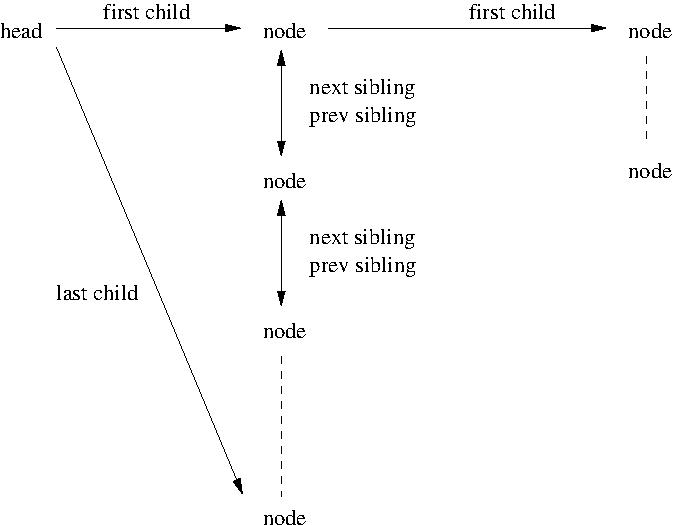
\includegraphics[width=.5\textwidth]{treefig}
\caption{Overview of the tree structure. The elements at the top of
the tree (here displayed at the left for convenience) are in the
``head'' (there can be more than one such element).  Every node is
linked to its children using the ``first child'' and ``last child''
links. In addition, all nodes on a given level are doubly-linked using
the ``previous sibling'' and ``next sibling'' links. The ``depth'' of
a given node refers to the horizontal distance from the head nodes.}
\label{f:overview}
\end{center}
\end{figure}

The tree class is templated over the data objects stored at the nodes;
just like you can have a {\tt vector<string>} you can now have a
{\tt tree<string>}. Many STL algorithms work on this data structure,
and where necessary alternatives have been provided.
\medskip

\end{sectionunit}
\begin{sectionunit}
\title{Iterators}
\maketitle

The essential difference between a container with the structure of a
tree and the STL containers is that the latter are ``linear''. While
the STL containers thus only have essentially one way in which one can
iterate over their elements, this is not true for trees. The {\tt
tree.hh} library provides (at present) four different iteration
schemes. To describe them, consider the following tree:
\begin{equation*}
\vcenter{\offinterlineskip
\halign{&#\mystrut\hfil\cr
 root \hw\cr
 \T A \cr
 \V   \T  B \cr
 \V   \L  C \cr
 \L D \cr
 \N   \T  E \cr
 \N   \L  F \cr}}
\end{equation*}
The three iteration types and the resulting order in which nodes are
visited are tabulated below:
\begin{center}
\begin{tabular}{llll}
pre-order (default) & ``element before children'' &
\member{pre\_order\_iterator}  & root A B C D E F \\
post-order          & ``element after children''  &
\member{post\_order\_iterator} & B C A E F D root \\
breadth-first &  &
\member{breadth\_first\_iterator} & root A D B C E F  \\
sibling             & ``only siblings'' & 
\member{sibling\_iterator} & (for ex.) A D \\
fixed-depth         & &
\member{fixed\_depth\_iterator} & (for ex.) A D \\
leaf                & &
\member{leaf\_iterator} & B C E F
\end{tabular}
\end{center}
The pre-order ones are the default iterators, and therefore also known
under the name of {\tt iterator}. Sibling iterators and fixed-depth
iterators iterate only over the nodes at a given depth of the
tree. The former restrict themselves to the child nodes of one given
node, while the latter iterates over all child nodes at the given
depth. Finally, leaf iterators iterate over all leafs (bottom-most)
nodes of the tree.

There are copy constructors that will convert iterators of the
various types into each other. The post- and pre-order iterators are
both also known as ``depth-first'', in contrast to the
``breadth-first'' iterator.

The begin and end iterators of a tree can be obtained using
\member{begin()} and \member{end()} (for pre-order iterators) or
alternatively \member{begin\_post()} and \member{end\_post()} (for
post-order iterators) and \member{begin\_leaf()} and
\member{end\_leaf()} (for leaf iterators). Similarly, the begin and
end sibling iterators can be obtained by calling
\member{begin(iterator)} and \member{end(iterator)}.  The range of
children of a given node can also be obtained directly from an
iterator, by using the {\tt iterator::begin()} and {\tt
iterator::end()} member functions.

If you want to (temporarily) make an iterator not go into the child
subtree, call the member function \member{skip\_children}. This will only
keep effect for a single increment or decrement of the
iterator. Finally, whether or not an iterator is actually pointing at
a node (i.e.~is not an ``end'' iterator) can be tested using the
\member{is\_valid(iterator)} member of the tree class.

\end{sectionunit}
\end{sectionunit}

\begin{sectionunit}
\title{Basic operations}
\maketitle
\begin{description}
\item[Initialising] There are two nontrivial constructors. One which takes 
a single node element as argument. It constructs a tree with this node
begin the sole node in the head (in other words, it is a combination
of a trivial constructor together with a \member{set\_head} call).
The other non-trivial constructor takes an iterator, and copies the
subtree starting at that node into the newly created tree (useful for
constructing new tree objects given by subtrees of existing trees).

\item[Tree traversal] Besides the \member{operator++} and
\member{operator--} members for step-wise traversal through the tree,
it is also possible to use the \member{operator+=} and \member{operator-=}
member functions to make more than one step at the same time (though
these are linear time, not amortized constant). The result of stepping
beyond the end of the tree or stepping beyond the end of a sibling
range (for sibling iterators) is undefined.

The parent of a given node can be reached by calling the \member{parent}
member of the tree object, giving it an iterator pointing to the node.

If you know the number of children of a given node, you can get direct
access to the $n$th child by using the \member{child} member
function. Note that the value of the index is not checked and should
therefore always be valid.

\item[Appending child nodes] Nodes can be added as children of a given
node using the \member{append\_child} member function.

\item[Inserting nodes] Nodes can be inserted at the same depth as a
given other node using the \member{insert} and \member{insert\_after}
members functions. This is also how you insert the first node into a 
tree.
\end{description}
\end{sectionunit}

\begin{sectionunit}
\title{Other algorithms}
\maketitle
\begin{sectionunit}
\title{Non-mutating algorithms}
\maketitle
\begin{description}
\item[Counting nodes] The total number of nodes of a tree can be
obtained using the \member{size} member function, while the number of
children of a given node can be obtained with a call to
\member{number\_of\_children(iterator)}. Similarly, the number of
nodes at a given depth (the number of siblings of a given node) can be
obtained using the \member{number\_of\_siblings} member function.
\item[Determining depth] The \member{depth()} member function returns the
distance of a node to the root.
\item[Accessing siblings by their index] See the next item.
\item[Determining index in a sibling range] In order to determine the
index of a node in the range of siblings to which it belongs, use the
\member{index(sibling\_iterator)} member function. The first sibling node
has index 0. The reverse of this function (obtaining a sibling node
given its index in the range of siblings) is called
\member{child(const iterator\_base\&, unsigned int)}.
\item[Comparing trees] While the STL \member{equal} algorithm can be used 
to compare the values of the nodes in two different trees, it does not 
know about the structure of the tree. If you want the comparison to
take this into account, use the \member{equal(iterator, iterator,
iterator, BinaryPredicate)} call of the tree class. As an addition to
the STL algorithm, the length of the first range does not have to be
equal to the length of the range pointed to by the second iterator.

There is also an \member{equal\_subtree} algorithm which takes only
two iterators, pointing to the (single-node) heads of two
subtrees.
\end{description}
\end{sectionunit}

\begin{sectionunit}
\title{Mutating algorithms}
\maketitle
\begin{description}
\item[Erasing nodes and subtrees] In order to remove a node including
its children from the tree, use the \member{erase(iterator)} call. If you
just want to erase the children, but not the node itself, use the 
\member{erase\_children(iterator)} call.

\item[Replacing individual nodes or subtrees] 

\item[Flattening subtrees] The procedure of moving all children of a
given node to be siblings of that node is called ``flattening''; it
acts as
\begin{equation*}
\vcenter{\offinterlineskip
\halign{&#\mystrut\hfil\cr
 apple \hw\cr
 \T banana\cr
 \V   \T  pear \cr
 \V   \T  strawberry \cr
 \V   \L  cherry \cr
 \L grape\cr}}\quad\rightarrow\quad
\vcenter{\offinterlineskip
\halign{&#\mystrut\hfil\cr
 apple \hw\cr
 \T banana\cr
 \T  pear \cr
 \T  strawberry \cr
 \T  cherry \cr
 \L grape\cr}}
\end{equation*}
% \begin{screen}
% apple                       apple
% 	  banana                      banana
% 		  pear            ->       pear
% 		  strawberry               strawberry
% 		  cherry                   cherry
% 	  grape                       grape
% \end{screen}
when the tree is flattened at the ``banana'' node.

\item[Moving or exchanging subtrees] Simple exchange of one sibling node with the
next one is done through the member function \member{swap(sibling\_iterator)}. The
iterator remains valid and remains pointing to the moved subtree.

More complicated move operations are the \member{move\_ontop},
\member{move\_before} and \member{move\_after} ones. These all take
two iterators, a source and a target. The member
\member{move\_ontop(target, source)} removes the `target' node and
all its children, and replaces it with the `source' node and its
children.  The `source' subtree is removed from its original location.
The other two move members do a similar thing, differing only in the
node which is to be replaced.

\item[Extracting subtrees] You can create a new tree object
filled with the data of a subtree of the original tree. This is
analogous to the extraction of a substring of a string. The relevant
member function is \member{subtree(sibling\_iterator,
sibling\_iterator)} which takes a range of siblings as argument. 
There is also a slight variation of this member, which does not return
a tree object but instead populates one that is passed as an argument
(useful if you want to call this on a tree object subclassed from
{\tt tree<T>}.

\item[Sorting] The standard STL sort algorithm is not very useful for
trees, because it only exchanges values, not nodes. Applying it to a
tree would mean that the structure of the tree remains unmodified,
only node values get moved around (not their subtrees).

Therefore, the {\tt tree} class has its own sort member. It comes in
two forms, just like the STL sort, namely
\begin{screen}
void     sort(sibling_iterator from, sibling_iterator to, bool deep=false);

template<class StrictWeakOrdering>
void     sort(sibling_iterator from, sibling_iterator to,
              StrictWeakOrdering comp, bool deep=false);
\end{screen}
The result of a call to either of these is that the nodes in the range
described by the two iterators get sorted. If the boolean {\tt deep}
is true, the subtrees of all these nodes will get sorted as well (and
so one can sort the entire tree in one call).  As in the STL, you can
use the second form of this function to pass your own comparison
class.

If the nodes to which the two iterators point are not in the same
sibling range (i.e.~not at the same depth in the tree), the result is undefined.

\item[Merging] One way in which one might think of indicating the
position where new nodes are to be inserted, is to give the path that
leads to the insertion point.  For instance, given the tree
\begin{equation*}
\vcenter{\offinterlineskip
\halign{&#\mystrut\hfil\cr
 apple \hw\cr
 \T banana\cr
 \V   \T  pear \cr
 \V   \T  strawberry \cr
 \V   \L  cherry \cr
 \L grape\cr}}
\end{equation*}
one could imagine using the sub-tree
\begin{equation*}
\vcenter{\offinterlineskip
\halign{&#\mystrut\hfil\cr
 apple \hw\cr
 \L banana\cr
 \N   \T  coconut \cr
 \N   \L  raspberry \cr}}
\end{equation*}
to indicate that the nodes ``coconut'' and ``raspberry'' are to be
inserted as new children of the ``banana'' node. In {\tt tree.hh} this
process is called \emph{tree merging}. It can do the simple addition
of children as above, but actually handles the generic case too: as
an example consider the merge
\begin{equation*}
\text{\tt merge}\left[
\vcenter{\offinterlineskip
\halign{&#\mystrut\hfil\cr
 apple \hw\cr
 \T banana\cr
 \V   \T  pear \cr
 \V   \T  strawberry \cr
 \V   \L  cherry \cr
 \T grape\cr
 blueberry \cr}}\quad, \quad
\vcenter{\offinterlineskip
\halign{&#\mystrut\hfil\cr
 apple \hw\cr
 \T banana\cr
 \V   \T coconut \cr
 \V   \L raspberry \cr
 \T tangerine \cr
 \V   \L plum\cr
 blueberry \cr
 \N   \L orange \cr}}\right]\quad\rightarrow\quad
\vcenter{\offinterlineskip
\halign{&#\mystrut\hfil\cr
 apple \hw\cr
 \T banana\cr
 \V   \T pear\cr
 \V   \T strawberry\cr
 \V   \T cherry\cr
 \V   \T coconut \cr
 \V   \L raspberry \cr
 \T grape\cr
 \T tangerine \cr
 \V   \L plum\cr
 blueberry \cr
 \N  \L orange \cr}}
\end{equation*}
As is clear from the above, the arguments to \member{merge} are two
sibling ranges.
\end{description}
\end{sectionunit}
\end{sectionunit}

\printindex
\end{document}

\cdbalgorithm{indexlist}{}

Displays a
list of all indices in an expression, together with their type
(dummy or free).

\end{algs}

\vfill\eject

% \subsection{Perturbative string theory ({\tt pertstring})}
% 
% 
% This module contains useful routines for the computation of
% perturbative string amplitudes, that is, it contains information about
% Jacobi theta functions and assorted things.
% \bigskip
% \begin{algs}
% \item[\cdbcommand{aticksen}{}] Work out a fermionic correlator according to
% \dcite{Atick:1987rs}. These correlators contain SO(2) spinors
% represented in the form of a complex fermion $\Psi$ and $\bar\Psi$, as
% well as spin fields $S_+$ and $S_-$ \kcomment{KP}{Lacking
% ``properties'', these currently have to be written as {\tt Psi}, {\tt
% Psibar}, {\tt Splus} and {\tt Sminus}.}. Correlators of these are written as
% {\tt \\corr\{...\}}, where the dots contain an arbitrary number of these
% fermionic fields, together with their dependence on insertion points. 
% The algorithm converts these correlators to Jacobi theta function expressions,
% (ignoring a normalisation constant) using the expression
% \begin{equation}
% \begin{aligned}[t] \Big\langle \prod_{i=1}^{N_1}& S^+(\tilde y_i)
% \prod_{i=1}^{N_2} S^-(y_i) \prod_{i=1}^{N_3} \bar\Psi(\tilde z_i)
% \prod_{i=1}^{N_4} \Psi(z_i)\Big\rangle_\nu \\[1ex]
% {} & = K_\nu  \frac{\displaystyle \prod_{i<j}\theta_1(\tilde y_i-\tilde y_j)^{\tfrac{1}{4}}
% \prod_{i<j} \theta_1(y_i-y_j)^{\tfrac{1}{4}} 
% \prod_{i<j} \theta_1(\tilde z_i-\tilde z_j)
% \prod_{i<j} \theta_1(z_i- z_j)}{\displaystyle
%   \prod_{i,j} \theta_1(y_i-\tilde y_j)^{\tfrac{1}{4}}
%   \prod_{i,j} \theta_1(z_i-\tilde z_i)
% } \\[1ex]
% & \quad\quad\times 
% \frac{ \displaystyle
%   \prod_{i,j} \theta_1(z_i-\tilde y_j)^{\tfrac{1}{2}}
%   \prod_{i,j} \theta_1(\tilde z_i - y_j)^{\tfrac{1}{2}}}{\displaystyle
%   \prod_{i,j} \theta_1(\tilde z_i- \tilde y_j)^{\tfrac{1}{2}}
%   \prod_{i,j} \theta_1(z_i-y_j)^{\tfrac{1}{2}}
% }\\[1ex]
% &\quad\quad\times
% \theta_\nu\left( \frac{1}{2}\sum_i \tilde y_i - \frac{1}{2}\sum_i y_i 
% + \sum_i z_i - \sum_i \tilde z_i\right)\, .
% \end{aligned}
% \end{equation}
% 
% \item[\cdbcommand{riemannid}{}] Implement the Riemann identity for
% a sum over spin structures of a product of four theta functions on the
% torus. That is, it implements
% \begin{multline}
% \sum_{\nu=1,2,3,4} (-)^{\nu-1}\, \theta_\nu(z_1|\tau) \theta_\nu(z_2|\tau)
% \theta_\nu(z_3|\tau) \theta_\nu(z_4|\tau) \\[1ex] = 
% 2\,
% \theta_1\left(\frac{z_1+z_2+z_3+z_4}{2}\Big|\tau\right)
% \theta_1\left(\frac{z_1+z_2-z_3-z_4}{2}\Big|\tau\right)\\[1ex]
% \times\theta_1\left(\frac{z_1-z_2-z_3+z_4}{2}\Big|\tau\right)
% \theta_1\left(\frac{z_1-z_2+z_3-z_4}{2}\Big|\tau\right)\, .
% \end{multline}
% In particular, if any the arguments coincide pairwise (e.g.~$z_1=z_2$
% and $z_3=z_4$) the right-hand side vanishes because $\theta_1$ is odd.
% \end{algs}
% 
% \vfill\eject

\subsection{General relativity}

This module deals with special tensors relevant for general
relativity. See in particular also the {\tt canonicalise} algorithm in
section~\ref{m:algebra}.
\bigskip
\begin{props}
\cdbproperty{Metric}{{\it signature={\sf integer}}}

Labels the object as a symmetric tensor, and optionally gives it the
indicated signature through the {\tt signature} parameter.
\begin{screen}{1,2,3}
g_{m n}::Metric(signature=1).
g_{m n} A^{n p};
@eliminate_metric!(%);
A_{m}^{p};
\end{screen}
Objects declared as \subsprop{Metrics} can be used to automatically
raise or lower indices using the
\subscommand{eliminate\_metric} command.

\cdbseealgo{eliminate_metric}

\cdbproperty{InverseMetric}{}

This property is the partner of \subsprop{Metric}. It makes the
associated two-tensor symmetric and also indicates that it can be used
to raise or lower indices.
\begin{screen}{1,2,3}
g^{m n}::InverseMetric.
g_{m n}::Metric.
g_{m q} g^{m n} A_{n p};
@eliminate_metric!(%);
A_{q p};
\end{screen}
For more information, see \subsprop{Metric}.

\cdbseealgo{eliminate_metric}
\cdbseeprop{Metric}
\cdbseeprop{Symmetric}

\cdbproperty{Vielbein}{}

Indicates that an object can be used to convert indices from one type
to another, i.e.~is a vielbein or tetrad. For more information, see
\subscommand{eliminate\_vielbein}.

\cdbseealgo{eliminate_vielbein}

\cdbproperty{InverseVielbein}{}

The partner of \subsprop{Vielbein}. See
the \subscommand{eliminate\_vielbein} command for more information on
typical usage patterns.

\cdbseeprop{Vielbein}
\cdbseealgo{eliminate_vielbein}

\cdbproperty{RiemannTensor}{}

Gives an object the symmetry properties of a Riemann tensor.
\begin{screen}{1,2}
R_{m n p q}::RiemannTensor;
A^{m n p}::AntiSymmetric.
A^{m n p} R_{m n p q};
@impose_bianchi!(%);
0;
\end{screen}
Various other algorithms, such as \subscommand{canonicalise}, also
take into account this property.

\cdbseealgo{canonicalise}
\cdbseealgo{impose_bianchi}

\cdbproperty{WeylTensor}{}

Gives an object the symmetry properties of a Weyl tensor, i.e.~a
Riemann tensor with an additional traceless condition. For more
information, see \subsprop{RiemannTensor}.

\cdbseeprop{RiemannTensor}


\end{props}
\bigskip
\begin{algs}
\cdbalgorithm{rewrite\_indices}{}

Rewrite indices on an object by contracting it with a second object
which contains indices of both the old and the new type (a vielbein,
in other words, or a metric). A vielbein example is
\begin{screen}{1,2,3,4}
{m,n,p}::Indices(flat).
{\mu,\nu,\rho}::Indices(curved).
T_{m n p};
@rewrite_indices!(%){ T_{\mu\nu\rho} }{ e_{\mu}^{n} };
T_{\mu \nu \rho} e_{\mu}^{m} e_{\nu}^{n} e_{\rho}^{p};
\end{screen}
If you want to raise or lower an index with a metric, this can also be
done with as an index rewriting command, as the following example shows:
\begin{screen}{1,2,3}
{m,n,p,q,r,s}::Indices(curved, position=fixed).
H_{m n p};
@rewrite_indices!(%){ H^{m n p} }{ g_{m n} };
H^{q r s} g_{m q} g_{n r} g_{p s};
\end{screen}
As these examples show, the desired form of the tensor should be given
as the first argument, and the conversion object (metric, vielbein) as
the second object. 

\cdbseealgo{split_index}

\cdbalgorithm{riemann\_index\_regroup}{}

Given a set (or multiple sets) of indices in which to anti-symmetrise,
this routine determines whether the indicated Riemann tensor has an
index distribution with two of the anti-symmetrised indices on two
different pairs. If so, it performs the substitution
\begin{equation*}
R_{m [p|\, n|q]} \rightarrow \frac{1}{2}R_{m n p q}\, ,
\end{equation*}
which is valid by virtue of the Riccy cyclic identity $R_{m [npq]}=0$.
The example above translates to
\begin{screen}{1,2,3,4}
R_{m n p q}::RiemannTensor.
A^{m n}::AntiSymmetric.
R_{m p n q} A^{p q};
@riemann_index_regroup!(%);
 1/2 R_{m n p q} A^{p q};
\end{screen}
Note that this also works on Weyl tensors.

\cdbseealgo{young_project_tensor}

\cdbalgorithm{ricci\_can\_order}{}

Rewrites all terms with 
two Weyl or Riemann tensors which are doubly contracted in a
canonical form, that is, with the contracted indices sitting on mixed
pairs. The identity that is used is
\begin{equation}
R_{a b m n} R_{c d m n} 
% = 2\, R_{a m n b} R_{c d m n}\, .
% = 2\, R_{a m n b} ( R_{c m n d} + R_{c n d m} )
 = 2\, R_{a m n b} ( R_{c m n d} - R_{d m n c} )\, .
\end{equation}

\cdbalgorithm{split\_index}{}

Replace a sum by a sum-of-sums, abstractly. Concretely, replaces all
index contractions of a given type by a sum of two terms, each with
indices of a different type. Useful for Kaluza-Klein reductions and
the like. An example makes this more clear:
\begin{screen}{1,2,3,4,5,7,8}
{M,N,P,Q,R}::Indices(full).
{m,n,p,q,r}::Indices(space1).
{a,b,c,d,e}::Indices(space2).
A_{M p} B_{M p};
@split_index(%){M,m,a};
A_{m p} B_{m p} + A_{a p} B_{a p};
@pop(%);
@split_index(%){M,m,4};
A_{m p} B_{m p} + A_{4 p} B_{4 p};
\end{screen}
Note that the two index types into wich the original indices should be
split can be either symbolic (as in the first case above) or numeric
(as in the second case).

\cdbseeprop{Indices}
\cdbseealgo{rewrite_indices}

\cdbalgorithm{split\_index}{}

Replace a sum by a sum-of-sums, abstractly. Concretely, replaces all
index contractions of a given type by a sum of two terms, each with
indices of a different type. Useful for Kaluza-Klein reductions and
the like. An example makes this more clear:
\begin{screen}{1,2,3,4,5,7,8}
{M,N,P,Q,R}::Indices(full).
{m,n,p,q,r}::Indices(space1).
{a,b,c,d,e}::Indices(space2).
A_{M p} B_{M p};
@split_index(%){M,m,a};
A_{m p} B_{m p} + A_{a p} B_{a p};
@pop(%);
@split_index(%){M,m,4};
A_{m p} B_{m p} + A_{4 p} B_{4 p};
\end{screen}
Note that the two index types into wich the original indices should be
split can be either symbolic (as in the first case above) or numeric
(as in the second case).

\cdbseeprop{Indices}
\cdbseealgo{rewrite_indices}

\cdbalgorithm{eliminate\_vielbein}{}

Eliminates vielbein objects.
\begin{screen}{1,2,3,4,5}
{ m, n, p }::Indices(flat).
{ \mu, \nu, \rho }::Indices(curved).
e_{m \mu}::Vielbein.
H_{m n p} e_{m \mu};
@eliminate_vielbein!(%){H_{\mu\nu\rho}};
H_{\mu n p};
\end{screen}
Other elimination commands of a similar type are
\subscommand{eliminate\_kr} for Kronecker delta symbols
and \subscommand{eliminate\_metric} for metric and inverse metric objects.

\cdbseealgo{eliminate_kr}
\cdbseealgo{eliminate_metric}

\cdbalgorithm{eliminate\_metric}{}

Eliminates metric and inverse metric objects.
\begin{screen}{1,2,3,4,5,6,7,8,10}
{m, n, p, q, r}::Indices(vector, position=fixed).
{m, n, p, q, r}::Integer(0..9).
g_{m n}::Metric.
g^{m n}::InverseMetric.
g_{m}^{n}::KroneckerDelta.
g^{m}_{n}::KroneckerDelta.
g_{m p} g^{p m};
@eliminate_metric!(%);
g^{p}_{p};
@eliminate_kr!(%);
10;
\end{screen}
Other elimination commands of a similar type are
\subscommand{eliminate\_kr} for Kronecker delta symbols
and \subscommand{eliminate\_vielbein} for vielbeine.

\cdbseealgo{eliminate_kr}
\cdbseealgo{eliminate_vielbein}

\end{algs}

\vfill\eject

\subsection{Substitution}

Substitution of expressions into other ones is a subtle issue. One
problem, namely that of relabelling of dummy indices, is addressed by
the core routines and has been discussed in section~\ref{s:dummies}. 
Here we will discuss how \cdb handles the issue of pattern matching.

%index label matching and product factor and sum term re-ordering.
\bigskip

\begin{algs}
\item[\cdbcommand{}{}] Given an expression number of label, this node
replaces itself with a copy of this expression. As with any active
node, this one takes care of dummy index relabelling automatically
(see section~\ref{s:dummies}).
\item[\cdbcommand{rename}{}] \outdated Renames objects and numbered objects,
but only on a fixed level, i.e.~does not do pattern matching at all.
For instance,
\begin{screen}{1,3}
F_{m1 m2 m3};
F_{m1 m2 m3}
@rename!(%){m}{r};
F_{r1 r2 r3}
\end{screen}
It will not prevent you from introducing dummy pairs:
\begin{screen}{1,2}
F_{m n};
@rename!(%){m}{n};
F_{n n};
\end{screen}
However, it will relabel already existing dummy pairs if you rename an
open index in such a way that it would conflict with the dummy pair:
\begin{screen}{1,2,3}
{m,n,p,q,r,s}::Indices(vector).
F_{m n} G_{n q};
@rename!(%){m}{n};
F_{n p} G_{p q};
\end{screen}
~
\cdbalgorithm{substitute}{}

 \label{loc_substitute} Generic substitution command.
Takes a rule or a set of rules according to which an expression
should be modified. If more than one rule is given, it tries each rule
in turn, until the first working one is encountered, after which it
continues with the next node.
\begin{screen}{1,2}
G_{mu nu rho} + F_{mu nu rho};
@substitute!(%)( F_{mu nu rho} -> A_{mu nu} B_{rho} );
G_{mu nu rho} + A_{mu nu} B_{rho};
\end{screen}
\begin{screen}{1,2}
A_{mu nu} B_{nu rho} C_{rho sigma};
@substitute!(%)( A_{m n} C_{p q} -> D_{m q} );
D_{mu sigma} B_{nu rho};
\end{screen}
This command takes full care of dummy index relabelling, as the
following example shows:
\begin{screen}{1,2,3}
{m,n,q,d1,d2,d3,d4}::Indices(vector).
a_{m} b_{n};
@substitute!(%)( a_{q} -> c_{m n} d_{m n q} );
c_{d1 d2} * d_{d1 d2 m} * b_{n};
\end{screen}
By postfixing a name with a question mark, it becomes a pattern.

The substitution algorithm can do very complicated things; for more
detailed information on substitution, see the manual.

\cdbseealgo{vary}

\cdbalgorithm{vary}{}

Generic variation command.  Takes a rule or a set of rules
according to which the terms in a sum should be varied. In every term,
apply the rule once to every factor.
\begin{screen}{1,2}
A B + A C;
@vary(%)( A -> \epsilon D,
          B -> \epsilon C,
          C -> \epsilon A - \epsilon B );
\epsilon D B + A \epsilon C + \epsilon D C 
                   + A (\epsilon A - \epsilon B);
\end{screen}
This algorithm is thus mostly intended for variational derivatives
(subsequent partial integrations can be done
using \subscommand{pintegrate}).

Note: In the example above, the command is applied only at the top
level (there is no exclamation mark used in the call
of \subscommand{vary}). To understand why this is important, compare
the following two examples. The first one works as expected,
\begin{screen}
A B;
@vary(%)( A -> a, B -> b);
a * B + A * b;
\end{screen}
In the second one, we add an exclamation mark,
\begin{screen}{1,2}
A B;
@vary!(%)( A -> a, B -> b);
0;
\end{screen}
The reason why we now get a zero is that in the first step, the vary
command acts in each of the individual factors, producing
\begin{screen}
a b;
\end{screen}
It then acts once more at the level of the product. But now there are
no uppercase symbols left anymore, and the variation produces zero.

\cdbseealgo{pintegrate}
\cdbseealgo{substitute}


\cdbalgorithm{take\_match}{}

Select a subset of terms in a sum or list which match the given
pattern. 
\begin{screen}{1,2}
A + B D G + C D A;
@take_match(%)( D Q?? );
B D G + C D A;
\end{screen}
In particular, note that the
{\tt Q??} is necessary to ensure that the pattern matches a product of
{\tt D} with something else. However, the algorithm has selected the
entire term, not just the part matched by the pattern; compare the
similar
\begin{screen}{1,2}
A + B D G + C D A;
@substitute!(%)( D Q?? -> 1);
A + G + A;
\end{screen}
in which the replacement is done on the pattern, not on the entire
term which contains the pattern.

This algorithm is particularly useful in combination with a copy
operation on the expression. It allows one to take out certain terms
from an expression, do manipulations on it, and then substitute it
back using \subscommand{replace\_match}.

The following example shows how this works by taking out the term
which contains a $\chi$ factor, doing a transformation on the $A_{m
n}$ tensor in that term, and then substituting back
using \subscommand{replace\_match}.
\begin{screen}{1,2,4,5}
expr:= A_{m n} \chi B^{m}_{p} + \psi A_{n p};
@take_match[@(%)]( \chi Q?? );
A_{m n} \chi B^{m}_{p};
@substitute!(%)( A_{m n} -> C_{m n} );
@replace_match!(expr)( \chi Q?? -> @(%) );
C_{m n} \chi B^{m}_{p} + \psi A_{n p};
\end{screen}
The \subscommand{replace\_match} pattern matching rules are identical
to those in \subscommand{take\_match}: a match always matches an entire
term, not just a factor of it.

\cdbseealgo{replace_match}
\cdbseealgo{substitute}


\cdbalgorithm{replace\_match}{}

Replaces a subset of terms in a sum or list which match the given
pattern. This is like a substitute, but always acting on entire terms. 
\begin{screen}{1,2}
A + B D G + C D A;
@replace_match!(%)( D Q?? -> 1);
A + 1;
\end{screen}
Note the difference with \subscommand{substitute},
\begin{screen}{1,2}
A + B D G + C D A;
@substitute!(%)( D Q?? -> 1);
A + G + A;
\end{screen}
See \subscommand{take\_match} for further details on how to use this
``select/modify/replace'' mechanism.


\cdbseealgo{take_match}
\cdbseealgo{substitute}


\end{algs}

\vfill\eject

\subsection{Linear algebra}

\begin{algs}
\cdbalgorithm{lsolve}{}

Solve a system of linear equations over integers. Example,
\begin{screen}{1,2}
{ a0+2*a2 + a3= 3, -a0 - a2 + a3= - (8/3) , a3 = 3};
@lsolve(%){a0,a2,a3};
{a0 = 34/3, a2 = (-17/3), a3 = 3};
\end{screen}
Underdetermined and inconsistent systems are handled as expected:
either some coefficients are left unfixed or the system is returned
and an error message is printed.

\cdbseealgo{decompose}

\cdbalgorithm{decompose}{}

Decompose a tensor monomial on a given basis of monomials. The basis
should be given in the second argument. All tensor symmetries,
including those implied by Young tableau Garnir symmetries, are taken
into account. Example,
\begin{screen}{0,1,2,3,5,6}
{m,n,p,q}::Indices(vector).
{m,n,p,q}::Integer(0..10).
R_{m n p q}::RiemannTensor.

R_{m n q p} R_{m p n q};
@decompose!(%)( R_{m n p q} R_{m n p q} );
{ -1/2 };
\end{screen}
Note that this algorithm does not yet take into account
dimension-dependent identities, but it is nevertheless already
required that the index range is specified.

\cdbseealgo{young_project_tensor}
\cdbseealgo{canonicalise}
\cdbseeprop{TableauSymmetry}

\end{algs}

\vfill\eject

\subsection{Gamma matrix algebra and fermions}

This module deals with manipulations of the Clifford algebra, spinor
representations of the Lorentz group and related issues. Cadabra
follows the conventions of Sevrin's appendix~1.5, except for the fact
that we call the time-like component zero and the product of all gamma
matrices~$\tilde\Gamma$.
\bigskip
\begin{props}
\cdbproperty{Spinor}{\it dimension={\sf integer},
type=Weyl$\vert$Majorana$\vert$MajoranaWeyl, chirality=Positive$\vert$Negative}

Declares an object to be a spinor, i.e.~transforming in one of the
spinor representations of the orthogonal or Lorentz group. The
declaration should involve an indication of the dimension, as in the
example below. It can optionally have type indicators (these should be
{\tt Majorana}, {\tt Weyl} or {\tt MajoranaWeyl}) and chirality
indicators for Weyl spinors ({\tt Positive} or {\tt Negative},
indicating the eigenvalue with respect to the generalised~$\gamma_5$
matrix). Here is an example:
\begin{screen}{1,2}
\psi::Spinor(dimension=11, type=Majorana).
\end{screen}
This property is taken into account by various algorithms such
as \subscommand{fierz} and \subscommand{spinorsort}.

\cdbseeprop{DiracBar}
\cdbseealgo{fierz}
\cdbseealgo{spinorsort}

\cdbproperty{DiracBar}{}

Declares an object to be the operator which applies the Dirac bar to a
spinor, i.e.~an operator which acts according to
\begin{equation}
\bar{\psi} = i \psi^\dagger \Gamma^0\,.
\end{equation}
For more information see e.g.~\subscommand{spinorsort} or \subscommand{fierz}.

\cdbseeprop{Spinor}
\cdbseealgo{spinorsort}
\cdbseealgo{fierz}

\cdbproperty{GammaMatrix}{\it metric={\sf metric name}}

A generalised generator of a Clifford algebra. With one vector index,
  it satisfies
\begin{equation}
\{ \Gamma^m, \Gamma^n \} = 2\,\eta^{mn}\,.
\end{equation}
The objects with more vector indices are defined as
\begin{equation}
\Gamma^{m_1\ldots m_n} = \Gamma^{[m_1}\cdots \Gamma^{m_n]}\,,
\end{equation}
where the anti-symmetrisation includes a division by~$n!$.
If you intend to use the \subscommand{join} algorithm, you have to add a
key/value pair \verb|metric| to set the name of the tensor which acts
as the unit element in the Clifford algebra.

\cdbproperty{GammaTraceless}{}

Declares a spinor object with a vector index to be zero when it is
contracted with a gamma matrix.

\cdbproperty{SigmaMatrix}{}

These are the invariant tensors relating the~$(\tfrac{1}{2},\tfrac{1}{2})$ to the vector representation of
SO(3,1). \Cdb uses the Wess~\& Bagger conventions,
which means that the metric has signature~$\eta = {\rm
  diag}(-1,1,1,1)$ and
\begin{equation}
(\sigma^{\mu})_{\alpha\dot{\beta}} = ( -{\mathbb 1}, \vec\sigma )_{\alpha\dot{\beta}}\,,\quad
(\bar{\sigma}^{\mu})^{\dot{\alpha}\beta} = (-{\mathbb 1}, -\vec\sigma)^{\dot{\alpha}\beta}\,.
\end{equation}
When the objects carry two vector indices, they are understood to be
\begin{equation}
(\sigma^{m n})_{\alpha}{}^{\beta} \equiv \frac{1}{4}( \sigma^m
  \bar{\sigma}^n - \sigma^n \bar{\sigma}^m)_{\alpha}{}^{\beta}\,,\quad\quad
(\bar{\sigma}^{m n})^{\dot{\alpha}}{}_{\dot{\beta}} \equiv
  \frac{1}{4}(\bar{\sigma}^m \sigma^{n}
- \bar{\sigma}^n \sigma^{m})^{\dot{\alpha}}{}_{\dot{\beta}}\,.
\end{equation}
See below for algorithms dealing with the conversion from indexed to
index-free notation.

\cdbproperty{SigmaBarMatrix}{}

See \subsprop{SigmaMatrix} for details.

\cdbseeprop{SigmaMatrix}

\end{props}
\bigskip
\begin{algs}
\cdbalgorithm{join}{}

Join two fully anti-symmetrised gamma matrix
products according to the expression
\begin{equation}
   \Gamma^{b_{1}\dots b_{n}}\Gamma_{a_{1}\dots a_{m}} =
      \sum_{p=0}^{\text{min}(n,m)}\ \frac{n! m!}{(n-p)! (m-p)! p!}
         \Gamma^{[b_{1}\ldots b_{n-p}}{}_{[a_{p+1}\ldots a_{m}}
         \eta^{b_{n-p+1}\ldots b_{n}]}{}_{a_{1}\ldots a_{m-p}]} \, .
\end{equation}
This is the opposite of \subscommand{gammasplit}.

Without further arguments, the anti-symmetrisations will be left
implicit. The argument ``{\tt expand}'' instead performs the sum over
all anti-symmetrisations, which may lead to an enormous number of
terms if the number of indices on the gamma matrices is large. Compare
\begin{screen}{1,2}
\Gamma{#}::GammaMatrix(metric=g).
\Gamma_{m n} \Gamma_{p};
@join!(%);
\Gamma_{m n p} + 2 \Gamma_{m} g_{n p};
\end{screen}
with
\begin{screen}{1,2}
\Gamma{#}::GammaMatrix(metric=g).
\Gamma_{m n} \Gamma_{p};
@join!(%){expand};
\Gamma_{m n p} + \Gamma_{m} g_{n p} - \Gamma_{n} g_{m p};
\end{screen}
Note that the gamma matrices need to have a metric associated to them
in order for this algorithm to work.

In order to reduce the number somewhat, one can instruct the algorithm
to make use of generalised Kronecker delta symbols in the result;
these symbols are defined as
\begin{equation}
\delta^{r_1}{}_{s_1}{}^{r_2}{}_{s_2}\cdots{}^{r_n}{}_{s_n}
= \delta^{[r_1}{}_{s_1}\delta^{r_2}{}_{s_2}\cdots {}^{r_n]}{}_{s_n}\, .
\end{equation}
Anti-symmetrisation is implied in the set of even-numbered
indices. The use of these symbols is triggered by the ``{\tt
gendelta}'' option,
\begin{screen}{1,2}
{m,n,p,q}::Indices(position=fixed).
\Gamma{#}::GammaMatrix(metric=\delta).
\Gamma_{m n} \Gamma^{p q};
@join!(%){expand}{gendelta};
 \Gamma_{m n}^{p q} + \Gamma_{m}^{q} \delta_{n}^{p} 
    - \Gamma_{m}^{p} \delta_{n}^{q} - \Gamma_{n}^{q} \delta_{m}^{p} 
    + \Gamma_{n}^{p} \delta_{m}^{q} + 2 \delta_{n}^{p}_{m}^{q};
\end{screen}

Finally, to select only a single term (for a given $p$) in this
expansion, give the join an argument with the value of $p$. 
\begin{screen}{1,2}
\Gamma{#}::GammaMatrix(metric=g).
\Gamma_{m n} \Gamma_{p};
@join!(%){expand}{3};
\Gamma_{m n p};
\end{screen}
This option can also be combined with {\tt gendelta} if required.

\cdbseeprop{GammaMatrix}
\cdbseeprop{KroneckerDelta}
\cdbseealgo{gammasplit}

\cdbalgorithm{gammasplit}{}

The opposite of \subscommand{join}: splits off a gamma matrix from a
totally anti-symmetrised product, e.g.
\begin{equation}
\Gamma^{mnp} = \Gamma^{mn}\Gamma^p - 2\,\Gamma^{[m} \eta^{n]}{}_p\, .
\end{equation}
In code this reads
\begin{screen}{1,2}
\Gamma{#}::GammaMatrix(metric=\eta).
\Gamma^{m n p};
@gammasplit(%);
 \Gamma^{m n} \Gamma^{p} - \Gamma^{m} \eta^{n p} 
                                  + \Gamma^{n} \eta^{m p};
\end{screen}
By default it splits of the one from the back, like in the example
above, but with argument {\tt front} it will split from the front:
\begin{screen}{1,2}
\Gamma{#}::GammaMatrix(metric=\eta).
\Gamma^{m n p};
@gammasplit(%){front};
\Gamma^{m} \Gamma^{n p} - \Gamma^{p} \eta^{m n} 
                                  + \Gamma^{n} \eta^{m p};
\end{screen}
~

\cdbseealgo{join}
\cdbseeprop{GammaMatrix}

\cdbalgorithm{rewrite\_diracbar}{}

Rewrite the Dirac conjugate
  of a product of spinors and gamma matrices as a product of Dirac
  and hermitean conjugates. This uses
  \begin{equation}
    \bar\psi = i \psi^\dagger\Gamma^0\,,
\end{equation}
together with 
\begin{equation}
  \Gamma_m^{\dagger} = \Gamma_0\Gamma_m\Gamma_0 \,.
\end{equation}
For example,
\begin{screen}{1,2,3,4,5}
\bar{#}::DiracBar.
\psi::Spinor(dimension=10).
\Gamma{#}::GammaMatrix.
\bar{\Gamma^{m n p} \psi};
@rewrite_diracbar!(%);
\bar{\psi} \Gamma^{m n p};
\end{screen}
~

\cdbseealgo{spinorsort}
\cdbseeprop{GammaMatrix}
\cdbseeprop{DiracBar}
\cdbseeprop{Spinor}

\cdbalgorithm{projweyl}{}

Projects an expression onto Weyl spinors of positive chirality (this
algorithm only works in even dimensions). On such a subspace, we have
\begin{equation}
\label{e:g10toeps}
\Gamma^{r_1 \cdots r_{d}}\Big|_{\text{Weyl}} = \frac{1}{\sqrt{-g}}\epsilon^{r_1\cdots
r_{d}}
\, ,\quad \epsilon^{0\cdots (d-1)} = +1\, ,
\end{equation}
and therefore all gamma matrices with more than $d/2$ indices can be
converted to their ``dual'' gamma matrices. By repeated contraction
of~\eqref{e:g10toeps} with gamma matrices on the left one deduces that
\begin{equation}
\Gamma^{r_1\cdots r_n}\Big|_{\text{Weyl}} = \frac{1}{\sqrt{-g}} \frac{(-1)^{\frac{1}{2}n(n+1)+1}}{(d-n)!}
\Gamma_{s_1\cdots s_{d-n}}\Big|_{\text{Weyl}} \epsilon^{s_1\cdots s_{d-n} r_1\cdots r_n}\, .
\end{equation}
Here is an example:
\begin{screen}{1,2}
{m,n,p,q,r,s,t}::Indices.
{m,n,p,q,r,s,t}::Integer(0..5).
\Gamma{#}::GammaMatrix.
\Gamma_{m n p q};
@projweyl!(%);
\end{screen}

\cdbseeprop{GammaMatrix}
\cdbseealgo{join}

\cdbalgorithm{spinorsort}{}

Sorts Majorana spinor bilinears using the Majorana flip property,
which for anti-commuting spinors takes the form
\begin{equation}
\bar\psi_1 \Gamma_{r_1\cdots r_n}\psi_2 = 
  \alpha \beta^n (-)^{\frac{1}{2}n(n-1)}\, \bar\psi_1
  \Gamma_{r_1\cdots r_n}\psi_2\, .
\end{equation}
Here $\alpha$ and $\beta$ determine the properties of the charge
conjugation matrix,
\begin{equation}
{\cal C}^T = \alpha {\cal C}\,,\quad
{\cal C}\Gamma_r {\cal C}^{-1} = \beta \Gamma_r^T\, .
\end{equation}
Here is an example.
\begin{screen}{1,2,3,4,5,6,7}
{\chi, \psi, \psi_{m}}::Spinor(dimension=10, type=MajoranaWeyl).
{\chi, \psi, \psi_{m}}::AntiCommuting.
\bar{#}::DiracBar.
\Gamma{#}::GammaMatrix.
{\psi_{m}, \psi, \chi}::SortOrder.
\bar{\chi} \Gamma_{m n} \psi;
@spinorsort!(%);
(-1) \bar{\psi} \Gamma_{m n} \chi;
\end{screen}
~
% These depend on dimension and are given by (some of these are choices)
% \kcomment{KP}{signature dependence!}
% \begin{equation}
% \begin{matrix}
%           & \alpha & \beta \\
%   d=4     &   -    &   -   \\
%   d=5     &   -    &   +   \\
%   d=6,1   &   +    &   -   \\
%   d=8     &   +    &   -   \\
%   d=10,1  &   -    &   -   
% \end{matrix}
% \end{equation}

\cdbseeprop{GammaMatrix}

\end{algs}


\vfill\eject

\subsection{Conversion from/to other formats}

\Cdb's syntax is a superset of the Maple and Mathematica formats, in
the sense that the internal tree representation of \cdb can store
input for both of these systems. However, this may not always be the
most convenient way of storage, as \cdb often has more compact or
expressive ways to store tensors. The {\tt convert} module provides
conversion algorithms from and to these two formats.
\bigskip

\begin{algs}
\cdbalgorithm{run}{}

Run an external program on the input expression, replacing it with the
standard output of the program. The expression is the first command
line argument of the program to be called.

Suppose we have a simple script {\tt test.sh} containing
\begin{screen}{0}
#!/bin/sh
echo "$1" | sed -e 's/A/B/g' -e '/;/q'
\end{screen}
This script replaces 'A' with 'B' in the first command line argument,
until it encounters a semi-colon.  We can then call this script by
using e.g.
\begin{screen}{1,2}
A B C A D E;
@run(%){"./test.sh"};
B B C B D E;
\end{screen}
The external program should make sure that it produces valid cadabra
input. 

\item[{\cdbcommand{from\_math}{}[expression]}] Reads mathematica input
format as used by GAMMA~\cite{Gran:2001yh}. Fully anti-symmetric
tensors are denoted with
\begin{screen}{0}
Tensor[name,{indices}]
\end{screen}
Tensors with property ``weyltensor'' are printed as
\begin{screen}{1}
W_{r1 r2 r3 r4}  
Weyl[{r1,r2}, {r3,r4}]
\end{screen}
(warning, this removes the tensor name).
\item[{\cdbcommand{to\_math}{}[expression]}] Converts the mathematica expression
to a \cdb one. See above for details about the conversion process.
\end{algs}



\vfill\eject

\section{Core functionality}

\subsection{Source file description}

The files in the {\tt src} directory build up the core of the program
and are described below. Algorithm-specific code is in the {\tt
src/modules} subdirectory and a description of those files can be
found in section~\ref{s:modules}. The files below should not be
changed when adding new modules.
\begin{description}
\item[{\tt main.cc}] Startup routines; initialises the I/O streams,
sets up the signal handlers for control-C and window resize signals
and starts the main event loop.

\item[{\tt manipulator.cc}, {\tt manipulator.hh}] Contains the object
  that processes the input line by line, activates the parser on it,
  and scans the tree for active nodes. A few very low-level commands
  (see section~\ref{s:builtin}) are handled in this class, while the
  other ones are dispatched to external modules.

\item[{\tt preprocessor.cc}, {\tt preprocessor.hh}] The code for
conversion of human editable infix input to the tree-form handled by
the other parts of the program. This is a text-to-text filter forming
the first pass of the parser. All functionality can be tested using
\verb|test_preprocessor.cc|.

\item[{\tt storage.cc}, {\tt storage.hh}] The node and tree classes
for storage of the tree form of expressions. These are the classes on 
which actual symbolic manipulation takes place. See also the separate
\verb|tree.hh| class.

\item[{\tt parser.cc}, {\tt parser.hh}] The class which contains the
parsing algorithms that turns output of the preprocessor class into a
tree form.

\item[{\tt algorithm.cc}, {\tt algorithm.hh}] The base class for all
the classes defined in the modules subdirectory. Plus the
implementation of scanning for command arguments and the necessary
logic to create the undo information, apply an algorithm until it no
longer changes the expression and other things which are independent
of the particular command.

\item[{\tt combinatorics.hh}] General routines for the generation of
combinations and permutations of elements in a vector. Consists
of a single class {\tt combinations<$\ldots$>} templated over the
type of the objects to be permuted. This class acts as a container
holding both the original vector (in the {\tt storage} member), the
permutation patterns (in the {\tt sublengths} vector, more on this
later) as well as the resulting permuted vectors (accessible through 
{\tt operator[]}; the total number of combinations is given by
{\tt size()}).
\end{description}

\subsection{Tree representation of expressions}
\label{s:internal_storage}

Expressions are internally stored in a tree container class, based on
the {\tt tree.hh} library~\cite{kas_tree}. The present section
describes the tree format in some more detail. 

Let us start with a couple of remarks on the motivation which has led
to the current implementation. An important requirement for the
storage format is that symbols should not have a fixed meaning, but
rather be like variables in a computer program: they can be declared
to represent objects of a certain type. Similarly, the user should be
free to use arbitrary bracket types and sub- and superscript
indicators (these should in addition be kept during the algebraic
manipulations). The first issue is resolved with the property system,
but the second one needs support directly in the storage tree.

Secondly, storage should be such that a trivial (often occurring)
extensions from one object to another should not lead to blowup. For
instance, the difference between \verb|A_\mu| and \verb|A_{\mu \nu}|
should preferably not introduce a new layer between the \verb|A| node
and the \verb|\mu| node. This is achieved by adding the bracket type
to the \emph{child} node rather than the parent (in the example above,
the curly brackets are part of the \verb|\mu| and \verb|\nu|
nodes). This applies also to e.g.~sums: in \verb|(A+B)| (which is
converted by the preprocessor to \verb|\sum(A)(B)| ), the round
brackets are part of the child nodes of the \verb|\+|
node.\footnote{Subsequent child nodes with the same bracket type
associated to them are taken to be part of the same group; the input
{\tt A\_\{$\backslash$mu\}\_\{$\backslash$nu\}} will therefore be
printed as {\tt A\_\{$\backslash$mu $\backslash$nu\}}. Similarly,
there is no way to represent $(a)+(b)$ since the internal storage
format automatically turns this into $(a+b)$.} Similarly, extending
\verb|q| to \verb|3q| should not introduce new intermediate layers to
group the two symbols together. This has been achieved by giving each
node a multiplier field (this holds true even for products,
i.e.~\verb|3(a+b)| is represented as a sum node with multiplier 3 (in
addition, such numerical factors are always commuted to the front of
the expression).\footnote{The multiplier field is a rational, and is
  intended to stay that way. It is not a good idea to make it
  complex, otherwise we will end up with octonionic multipliers at 
some stage. }
%We need some pre-defined symbols
%for $i$ and so on though, and rules to simplify products of
%them. These rules can be kept explicit and user-switchable to be
%automatic.}

It should also be possible to make expressions arbitrarily deeply
nested; one should be able to write \verb|a+b| as well as
\verb|\sin(a+b)|. This is in contrast to programs such as 
{\tt Abra} and {\tt FORM} which store their input as sums of products 
of factors, i.e.~without further nesting.

Finally, tt should be posssible to store the history of an expression,
in order to implement unlimited undo. 

The data stored at each tree node is further explained in
section~\ref{s:writing_new}, see in particular the excerpt from the {\tt
  storage.hh} file in figure~\ref{f:str_node}. The structure of the
actual tree is illustrated in figure~\ref{f:example_history}. 
Each expression starts with a {\tt history} node. The label of the
expression is given in a subnode {\tt label}. All remaining child
nodes of the {\tt history} nodes represent the history of the
expression. The most often encountered node here is the {\tt
  expression} node, which contains the actual expression. However,
there are other nodes as well, for instance {\tt asymimplicit} which
contains information about the symmetry structure of an expression
(this feature is not yet enabled).

\begin{figure}[t]
\begin{equation*}
\vcenter{\offinterlineskip
\halign{&#\mystrut\hfil\cr
\texcommand{history} \cr
\T  \texcommand{label}\cr
\V  \L  apple \cr
\T  \texcommand{expression} \cr
\V  \L  \texcommand{prod} \cr
\V  \N \T  a \cr
\V  \N \L  \texcommand{sum} \cr
\V  \N \N \T  b \cr
\V  \N \N \L  c \cr
\L  \texcommand{expression} \cr
\N  \L  \texcommand{sum} \cr
\N  \N  \T  \texcommand{prod} \cr
\N  \N  \V  \T  a \cr
\N  \N  \V  \L  b \cr
\N  \N  \L  \texcommand{prod} \cr
\N  \N  \N  \T  a \cr
\N  \N  \N  \L  c \cr }}
\end{equation*}
\caption{Example history tree for a single expression.  Here, the
program started with the user entering the expression $a (b+c)$. This
expression was then manipulated by applying the
\subscommand{distribute} algorithm. The nodes at the top of the
expression tree are all of the {\tt history} type.
\label{f:example_history}}
\end{figure}
% \T \texcommand{action}\cr
% \V  \T \subscommand{exchange}\cr
% \V  \N  \T a\cr
% \V  \N  \L b\cr
% \quad\quad\longleftrightarrow\quad\quad
% \vcenter{
% \offinterlineskip
% \halign{&#\mystrut\hfil\cr
% (1) $a+b$ \cr
% \T  exchange \cr
% \V  \L \,$b+a$\cr
% \V  \N \,rmult $d$\cr
% \V  \N \L \,$(b+a) d$ $\bullet$\cr
% \L  lmult $c$\cr
% \N  \L \,$c(a+b)$ \cr}}

\subsection{Nested sums, products and pure numbers}

Nested sum and product nodes require some explanation, as the way in
which \cdb handles and stores these determines how brackets can appear
in sums and products. As a general rule, sums within sums which are
such that all child nodes have the same, non-visible bracket are not
allowed, and automatically converted to a single sum. In other words
\begin{screen}{0}
(\sum{a}{b}+\sum{c}{d})
\end{screen}
is not allowed, since it would print as \verb|(a+b+c+d)| which is
indistinguishable from 
\begin{screen}{0}
(\sum{a}{b}{c}{d}) .
\end{screen}
The first expression is therefore internally always converted to the
second one before it is stored. A similar situation occurs with
products, where
\begin{screen}{0}
\prod{a}{\prod{b}{c}}
\end{screen}
is not allowed and ``flattened'' to the simpler
\begin{screen}{0}
\prod{a}{b}{c} .
\end{screen}
The general rule is that nested sums and products are converted to
flattened form if these two forms are indistinguishable in the
standard output format. Nested sums and products can occur, but they
have to have different or non-empty bracket types for their
children. An example is
\begin{screen}{0}
\prod{a}{\prod(b)(c)}
\end{screen}
which prints as \verb|a*(b*c)|. This is not automatically converted to
\verb|a*b*c|. Note that this form is \emph{not} represented as
\begin{screen}{0}
\prod{a}(b)(c)    (wrong)
\end{screen}
This is a consequence of the second rule: all child nodes of product
or sum nodes must have the same bracket type.  In summary, automatic
flattening of nested sum or product trees do not automatically occur
over bracket boundaries. You can then write and keep
$(\sin(x)+\cos(x)) + (\sin(x) + 3 \cos(x))$, which will be stored as
\begin{screen}{0}
\sum{\sum(sin(x))(cos(x))}{\sum(sin(x))(cos(x))}
\end{screen}
In order to remove brackets, one uses the \subscommand{sumflatten} 
and \subscommand{prodflatten} commands, see section~\ref{m:algebra}.

Products and sums with sub- or superscripts which apply to one or more
of the child nodes are internally represented using
\verb|\indexbracket| nodes. That is, the input
\begin{screen}{0}
q (a+b)_\mu
\end{screen}
is represented as
\begin{screen}{0}
\prod{q}{\indexbracket{\sum(a)(b)}_{\mu}}
\end{screen}
(note the way in which the bracket types are inherited).
In fact, such indexbracket constructions apply for any content inside
the brackets; in the example above, an indexbracket would be generated
even without the \verb|\sum| node: the input
\begin{screen}{0}
q (\Gamma^r)_{a b}
\end{screen}
is stored as
\begin{screen}{0}
\prod{q}{\indexbracket(\Gamma^r)_{a b}}
\end{screen}
The result of the indexbracket way of storing expressions is that
``index free'' manipulations apply directly inside the indexbracket
argument and no special algorithms are needed. Input will
automatically be converted to this form. Getting rid of indexbrackets
around single symbols is done using \subscommand{remove\_indexbracket}.

Another issue is the storage of numbers.  Since pure numerical factors
are only allowed to appear in the multiplier field of a node, a pure
number is stored as ``1'' with its multiplier equal to the
number. Product nodes with two arguments of which one is a number are
not allowed and will be converted to a single node with multiplier
field, automatically.

In order to eliminate ambiguities concerning multipliers in sum and
product nodes, the following rules should be obeyed: sum nodes always
have unit multiplier (i.e.~non-trivial multipliers are associated to
the children) and children of product nodes should also always have
unit multiplier (i.e.~the multipliers of all the children should in
this case be collected in the prod node itself).

\subsection{External scalar engine interface}

\Cdb is a tensor computer algebra system, without much functionality
for simplification or manipulation of scalar expressions. Other
systems exist which handle this much better, and it is a waste to
duplicate those efforts. Therefore, the \cdbclass{algorithm} class
contains functionality to isolate scalar factors from a tensorial
expression, manipulate them using an external scalar CAS, and
re-insert them into the internal \cdb tree.

Scalar expressions are defined to be sums or (subsets of factors of)
products which contain no objects with subscript or superscript
children (i.e.~contain no tensors). 

Exporting a scalar expression to an external CAS requires a rewriting
step before and after the export. At present only Maxima's format is
supported.



\vfill\eject

\section{Module implementation guide}


\subsection{Storage of numbers and strings}

There is a special memory area for the storage of rational numbers
(with arbitrary-length integers for the numerator and denominator) as
well as for the storage of strings. 

\subsection{Accessing indices}

Indices are stored as ordinary child nodes. However, there are various
ways to iterate over all indices in a factor, which are more useful
than a simple iteration over all child nodes. 

\subsection{Object properties}

The properties attached to a node in the tree can be queried by using
a lookup method in the {\tt properties} namespace. Object properties
are child classes of the {\tt property} class, and contain the
property information in a parsed form. The following code snippet
illustrates how properties are dealt with:
\begin{screen}{0}
AntiSymmetry *s=properties::get<AntiSymmetry>(it)
if(s) {
   // do something with the property info
   }
\end{screen}
Here we used a property called {\tt AntiSymmetry}, which is declared
in the the module header {\tt modules/algebra.hh} (see the other
header files of the various modules for information about the
available property types). If the node pointed to by {\tt it} has this
property associated to it, the pointer {\tt s} will be set to point to
the associated property node.  \bfcomment{KP}{Better to use a property
  example where the property node contains some additional
  information, which can then be used.}

It is also possible to do this search in the other direction, that is,
to find an object with a given property. 
\begin{screen}{0}
properties::property_map_t::iterator 
               it=properties::get_pattern<GammaMatrix>();
if(it!=properties::props.end()) {
   // Now *(it->first) contains the name of a GammaMatrix object.
   }
\end{screen}
\bfcomment{KP}{Instead of checking these things, it is better to throw
exceptions, since that will make the code more readable and also the
error handling more uniform (it can go in one place instead of being
repeated).}

Sums and products inherit, in a certain way, properties of the terms
and factors from which they are built up. This is true also for other
functions. If you want to know whether a given node has such
\emph{inherited properties}, a simple call to \verb|get<...>| is not
sufficient. Instead, use the following construction:
\begin{screen}{0}
Matrix *m=properties::get_composite<Matrix>(it)
if(m) {
   // do something with the property info
   }
\end{screen}
These inheritance rules for composite objects are at present
hard-coded but will be user-defineable at a later stage.



% \begin{sectionunit}
% \title{Labelling and selection of expressions}
% 
% 
% The kernel of \cdb is completely separated from its user interface,
% but the communication between the two uses a human-readable format.
% In order to allow the front-end to refer to individual elements of
% the expressions, a simple labelling scheme is used for every 
% node in an expression. The \cdb kernel output thus looks like
% \begin{screen}{0}
% \Gamma@1_{m@2} \Gamma@3_{n@4} \Gamma@5_{p@6}
% \end{screen}
% All symbols have been labelled with a unique
% numerical identifier. When you select the two gamma symbols, the
% front-end notifies the core of this action by sending back the
% identifiers ``1'' and ``3''. Upon receipt of the command {\tt @join}
% the core then knows to which objects this algorithm should apply.  In
% the absence of a front-end, you can do the selection by hand: just
% send the command {\tt @select} to the core, followed by a comma
% separated bracketed argument list of numerical identifiers. There also
% exist an {\tt @unselect} command.
% 
% 
% 

\subsection{Writing a new algorithm module}
\label{s:writing_new}

All functionality of cadabra that goes beyond storage of the
expression trees is located in separate modules, stored in the
\verb|src/modules| subdirectory. New functionality can easily be added
by writing new modules. All algorithm objects derive from the
\verb|algorithm| object defined in \verb|src/algorithm.hh|, and only
a couple of virtual members have to be implemented.
\begin{figure}[p!]
\begin{screen}{0}
class str_node {
   public:
      ...
};
\end{screen}
\caption{The node class.\label{f:str_node}}
\end{figure}
\begin{figure}[p!]
\begin{screen}{0}
class algorithm {
  public:
    typedef exptree::iterator         iterator;
    typedef exptree::sibling_iterator sibling_iterator;
  
    algorithm(exptree&, iterator&);
  
    virtual void     description() const=0;
    virtual bool     can_apply(iterator&);
    virtual bool     can_apply(sibling_iterator&, sibling_iterator&);
    virtual result_t apply(iterator&);
    virtual result_t apply(sibling_iterator&, sibling_iterator&);

    sibling_iterator args_begin() const;
    sibling_iterator args_end() const;
    unsigned int     number_of_args() const;

    exptree&  tr;
    iterator this_command;
};
\end{screen}
\caption{The relevant members of the class interface for the {\tt algorithm}
  object. The virtual members and the constructor have to be
  implemented in new algorithm objects; see the main text for an
  explanation of the two versions of {\tt can\_apply} and {\tt apply}.}
\label{f:algorithm}
\end{figure}
\begin{figure}[p!]
\begin{screen}{0}
class exptree {
  public:
    sibling_iterator arg(iterator, unsigned int) const;
    unsigned int     arg_size(sibling_iterator) const;
    multiplier_t     arg_to_num(sibling_iterator, unsigned int) const;
};
\end{screen}
\caption{The relevant members of the class interface for the {\tt exptree}
object.}
\end{figure}

The class interface for the algorithm object is shown in
figure~\ref{f:algorithm}.  The members which any class derived from
{\tt algorithm} should implement are described below.
\begin{description}
\item[{\tt constructor(exptree\&, iterator)}] Algorithm objects get
initialised with a reference {\tt tr} to the expression tree on which
they act, together with an iterator {\tt this\_command} pointing to
the associated command node. By looking at the child nodes of the
latter, the arguments of the command can be obtained. The simplest way
to do this is to use the sibling iterators returned by
\verb|args_begin()| and \verb|args_end()|; these automatically skip
the argument which refers to the equation number (i.e.~they skip the
\verb|(5)| argument in \verb|@command(5){arg1}{arg2}|). The
constructor is a good place to parse the command arguments, since that
will in general only be required once. Do not do anything in the
constructor that has to be done on every invocation of the same
command on different expressions.

If you discover that the arguments passed to an algorithm are 
not legal, you have to throw an {\tt algorithm::constructor\_error}
exception.
\item[{\tt description()}] Should display an explanation of the
functionality of the algorithm on the {\tt txtout} stream. Do not
add \verb|std::endl| newlines by hand, these will be inserted
automatically.
\item[\vbox{\hbox{\tt bool can\_apply(iterator)}
            \hbox{\tt bool can\_apply(sibling\_iterator, sibling\_iterator)}}] 
Determines whether the algorithm has a chance
of acting on the given expression. This is an \emph{estimate} but is
required to return {\tt true} if there is a possibility that the
algorithm would yield a change.  

It takes two sibling\_iterators as arguments, which indicate a node or
a range of nodes on which the algorithm is supposed to act.

Since {\tt can\_apply} is guaranteed to be called before {\tt apply},
it is allowed for the {\tt can\_apply} member to store results for later use in
{\tt apply}. However, multiple calls to can be made to this combo, so
any data stored should be erased upon each call to {\tt can\_apply}.
\item[\vbox{\hbox{\tt apply\_result apply(iterator\&)}
            \hbox{\tt apply\_result apply(sibling\_iterator\&, sibling\_iterator\&)}}]
Before exiting this function, the member variable {\tt
expression\_modified} has to be set according to whether or not the
apply call made any changes to the expression.

If the algorithm can take a long time to complete and you want to give
the user the option of interrupting it with control-C, you can check
(at points where the algorithm can be interrupted) the global variable
{\tt interrupted}. If it is set, you should immediately throw an
exception of type {\tt algorithm\_interrupted}, preferably with a
short string describing the location or algorithm at which the
interrupt occurred. The exception will be handled at the top level in
the {\tt manipulator.cc} code, where the current expression will be
removed. 
%
%Do not forget to unset it afterwards. If you exit an
%algorithm this way, your module should leave the expression tree in
%exactly the same way as it was when the {\tt apply} member was
%entered. Return \verb|l_error| to signal failure.

Algorithms can write progress information to the stream {\tt txtout}
and debug information (which will go into a separate file on disk) to
{\tt debugout}. These are global objects. Do not use the \Cpp streams
{\tt std::cout} and {\tt std::cerr} for this purpose.
\end{description}
An algorithm is \emph{never} allowed to modify the tree above the node
or range of sibling nodes which were passed to the \verb|apply|
call. In other words, siblings and parent nodes should never be
touched, and the nodes should not be removed from the tree
directly. If you want to remove nodes, this can be done by setting
their multiplier field to zero; the core routines will take care of
actually removing the nodes from the tree. It is allowed to inspect
the tree above the given nodes, but this is discouraged.

Upon any exit from an algorithm module, the tree is required to be in
a valid state. In many cases, it is useful to clean up modifications
to the tree by calling the utility function {\tt cleanup\_expression}
(see section~\ref{s:utility} for more information).


\subsection{Adding the module to the system}

Once you have written the \verb|.hh| and \verb|.cc| files associated
to your new algorithm, it has to be added to the build process and the
core program. First, add the header to the master header file
\verb|src/modules/modules.hh| file; this one looks like
\begin{screen}{0}
src/modules/modules.hh:

#include "algebra.hh"
#include "pertstring.hh"
#include "select.hh"
...
\end{screen}
You also have to add it to the \verb|src/Makefile.in|. Near the top of
this file you find a line looking somewhat like
\begin{screen}{0}
src/Makefile.in:

...
MOBJS=modules/algebra.o modules/pertstring.o modules/convert.o \
      modules/field_theory.o modules/select.o modules/dummies.o \
      modules/properties.o modules/relativity.o modules/substitute.o
...
\end{screen}
and this is where your module has to be added. Finally, you have to
make the algorithm visible to the core program. This is done in the
\verb|src/manipulator.cc| file. In the constructor of the
\verb|manipulator| class (defined somewhere near the top), you see a
map of names to algorithm classes. A small piece is listed below:
\begin{screen}{0}
src/manipulator.cc:

...
// pertstring
algorithms["@aticksen"]       =&create<aticksen>;
algorithms["@riemannid"]      =&create<riemannid>;

// algebra
algorithms["@distribute"]     =&create<distribute>; 
 ...
\end{screen}
Add your algorithm here; it does not have to have the same name as the
object class name. Once this is all done, rerun configure and make.


\subsection{Adding new properties}

\begin{figure}[t]
\begin{screen}{0}
class property\_base{
  public:
    virtual bool        parse(exptree&, iterator pat, iterator prop);
    virtual std::string name() const=0;
    virtual void        display(std::ostream&) const;
};

class property      : public property\_base {};
class list\_property : public property\_base {};

class labelled\_property : public property {
  public:
    std::string label;
};
\end{screen}
\caption{The relevant members of the class interface for the {\tt
	 property\_base} object and the derived objects.}
\end{figure}

\bfcomment{KP}{Discuss the various member functions of property, in
particular the way in which parse is supposed to behave, and the way
in which properties should be registered.}
Since algorithms rely crucially on a \emph{fixed} set of properties
which they provide themselves, we store these things in a \Cpp way,
rather than using strings. Another motivation: we do not want to parse
(and check) these property trees every time they are accessed. 

Properties typically carry key/value pairs which further specify 
the characteristics of the property. When the property object is
created, the core calls the \verb|parse()| method of the property, in
which you are responsible for scanning through the list of key/value
pairs. This is rather simple: just call the \verb|find()| member of
the \verb|keyval| argument,
\begin{screen}{0}
keyval_t::iterator ki=keyvals.find("dimension");
if(ki!=keyvals.end()) {
    // now ki->second is an iterator to an expression subtree
    }
\end{screen}
If the new property is derived from existing ones, do not forget
to call the \verb|parse()| method of all parent classes at the end.

Once this is all done, register the property with the system by adding
an appropriate call to the module's \verb|register_properties()|
method, found at the top of each module.

\subsection{Throwing errors}

If, at any stage, an inconsistent expression is encountered, the safe
way to return to the top level of the manipulator is to throw the
exception class \cdbclass{consistency\_error} (defined in \cdbfile{algorithm.hh}).


\subsection{Manipulating the expression tree}

The \cdbclass{exptree} class contains a number of tree access routines
which enhance the functionality of the {\tt tree.hh} library. 
\begin{description}
\item[\member{index\_iterator}] 
\item[\member{index\_map\_t}]
\end{description}

\subsubsection{Acting on products or single terms}

use \member{is\_single\_term} and \member{prod\_wrap\_single\_term}.


\subsection{Utility functions}

\label{s:utility}
There are also various useful helper functions in the {\tt exptree} 
class, mainly dealing with the conversion of expression numbers or
labels to iterators that point to the actual expression in the tree.
\begin{description}
\item[\vbox{\hbox{\member{cleanup\_expression(exptree\&)}}
            \hbox{\member{cleanup\_expression(exptree\&, iterator)}}}]
Converts an expression (or part of it below the indicated node) to
a valid form. That is, it calls various simplification algorithms
on the expression, among which {\tt sumflatten} and {\tt prodcollectnum}. 

\item[\member{cleanup\_nests}] When called on a product inside a
  product, or a sum inside a sum, and the bracket types of both node
  and parent are the same, flatten the tree. Adjusts the iterator to
  point to the product or sum node which remains.

\item[\member{equation\_by\_number\_or\_name}] Given an iterator
to a node that represents an expression number or expression label,
this member returns an iterator that points to the actual node
(to be precise: to the \verb|\history| node of the expression).

\item[\vbox{\hbox{\member{arg\_size(sibling\_iterator)}}
      \hbox{\member{arg(iterator, unsigned int)}}}]
Many algorithms require one \emph{or more} objects as arguments. These
are usually passed as lists, and therefore end up being of two forms:
either they are single objects or they are {\tt comma} objects
representing a list. In order to avoid having to check for these two
cases, one can use these two member functions.

The iterator arguments of these two member functions should point to
the child which is either a single argument or a \texcommand{comma}
node.

\item[\member{pushup\_multiplier}] Can be called on any node. If the
  node has a non-unit multiplier and the storage conventions exclude
  this, the algorithm will push the multiplier up the tree.
\end{description}
% \begin{itemize}
% \item The various comparison functions in str\_node.
% \item Members of active\_node and algorithm.
% \item Multiply, add, zero and one in these classes.
% \end{itemize}


\subsection{Writing a new output module}


\kcomment{KP}{Structure is different now: one inherits from {\tt
output\_exptree} and then has printing stuff at ones disposal. Still
would be nice to be able to change the printing objects for a given
node type, i.e.~modify the map of node names to printing objects.}

\kcomment{KP}{Also do something intelligent with the Mathematica
output flags}.


\subsection{Namespaces and global objects}

The following objects are global:
\begin{description}
\item[{\tt modglue::opipe txtout}] 
The normal output stream, to which you should communicate with the user.
\item[{\tt std::ofstream debugout}]
The debug output stream, which normally writes to a file, and should
only be used to write output which is useful for debugging purposes.
\item[{\tt nset\_t name\_set}]
The global collection of all strings. Nodes in the expression tree
contain an iterator into this map (see in particular figure~\ref{f:str_node}).
\item[{\tt rset\_t rat\_set}]
The global collection of all rational numbers. Nodes in the expression
tree contain an iterator into this map (see in particular figure~\ref{f:str_node}).
\item[{\tt bool interrupted}]
A global flag which indicates that the user has requested the
computation to be interrupted. See section~\ref{s:writing_new} for
more information on this variable.
\item[{\tt stopwatch globaltime}]
The wall time since program start.
\item[{\tt unsigned int size\_x, size\_y}] The size of the current
  output window.
\end{description}

% \subsection{Troubleshooting}
% 
% \begin{description}
% \item[Problems getting expressions in canonical form]
% There are various canonical places to look for errors. One of
% them is the routine {\tt propagate\_zeroes}, which may still not remove
% zeroes properly but leave an inconsistent tree. Another place
% is {\tt cleanup\_nests}.
% \end{description}
\vfill\eject

% \section{Future plans}
% \subsection{Front-ends}
% 
% 
% %The text-mode front-end will be based on {\tt eqascii} by
% %\dcite{e_bori1}, while the graphical front-end will use 
% %\TeX{} for typesetting.
% 
% \subsection{Component calculations}

%\vfill\eject


% \begin{sectionunit}
% \title{Using the history mechanism}
% 
% Let us first discuss an example which shows the way in which the \cdb
% history mechanism works, and also exhibits the selection mechanism. 
% As with all other data structures in \cdb, the history is also a
% tree-like structure. Expressions and commands get appended as children
% of each other. When you backtrack by going to a previous expression in
% the history, any new commands get added as child, thereby keeping
% the previous calculations based on that node accessible. An
% example illustrates how this works.
% \begin{screen}{0}
% > \Gamma_{m} \Gamma_{n}
% 	 (1)    : \Gamma_{m} \Gamma_{n}
% > @join{(1), 1, 2}
% 	 (1)    : \Gamma_{m n} + \eta_{m n}
% > \Gamma_{m n} = \epsilon_{p q r s} \Gamma^{p q r s} \tilde\Gamma
% 	 (1)    : \Gamma_{m n} + \eta_{m n}
% 	 (2)    : \Gamma_{m n} = \epsilon_{p q r s m n} \Gamma^{p q r s} \tilde\Gamma
% > @subs{(2), (1)}
% 	 (1)    : \epsilon_{p q r s m n}\Gamma^{p q r s}\tilde\Gamma + \eta_{m n}
% 	 (2)    : \Gamma_{m n} = \epsilon_{p q r s} \Gamma^{p q r s} \tilde\Gamma
% > \eta_{m n} = 0
% 	 (1)    : \epsilon_{p q r s m n}\Gamma^{p q r s}\tilde\Gamma + \eta_{m n}
% 	 (2)    : \Gamma_{m n} = \epsilon_{p q r s} \Gamma^{p q r s} \tilde\Gamma
% 	 (3)    : \eta_{m n} = 0
% > @up((1))
% 	 (1)    : \Gamma_{m n} + \eta_{m n}
% > @subs{(3), (1)}
% 	 (1)    : \Gamma_{m n}
% 	 (2)    : \Gamma_{m n} = \epsilon_{p q r s} \Gamma^{p q r s} \tilde\Gamma
% 	 (3)    : \eta_{m n} = 0
% \end{screen}
% Notice how the modification of equation~(1) has produced a new
% equation, but it has kept the original expression in memory as well.
% You can see the history of an equation by doing
% \begin{screen}{0}
% > @showtree((1))
% 	 input
% 	 (1)         : \Gamma_{m} \Gamma_{n}
% 		join
% 		(1.1)     : \Gamma_{m n} + \eta_{m n}
% 		  subs
% 		  (1.1.1) : \epsilon_{p q r s m n}\Gamma^{p q r s}\tilde\Gamma + \eta_{m n}
% 		  subs
% 		  (1.1.2)*: \Gamma_{m n}
% \end{screen}
% The star indicates which equation is currently denoted with~(1) in the
% compact output. If you are not interested in the paths that led to
% other expressions, then it is sufficient to do
% \begin{screen}{0}
% > @showhistory((1))
% 	 input  : \Gamma_{m} \Gamma_{n}
% 	 join   : \Gamma_{m n} + \eta_{m n}
% 	 subs   : \Gamma_{m n}
% \end{screen}
% This can be used to generate a clean report of all the manipulations
% that lead up to a certain result. If you are confident that you do not
% anymore need any of the branches except the one that leads to the
% last result, you can enter the \verb|@cleanhistory| command.
% 




\printindex
\bibliographystyle{kasper}
\bibliography{kasbib}
\end{document}





% \begin{sectionunit}
% \title{Cursor mode}
% 
% At any time, pressing `escape' will jump to the `cursor' mode. In this
% mode, one can select and unselects parts of the expression. Available
% commands:
% \begin{center}
% \begin{tabular}{ll}
% cursor-right & move cursor to next object on this level \\[1ex]
% cursor-left  & move cursor to previous object on this level \\[1ex]
% cursor-down  & move cursor to the arguments of the current
% objects\\[1ex]
% cursor-up    & move cursor to the parent of the current object\\[1ex]
% page-down    & enlarge cursor size \\[1ex]
% page-up      & shrink cursor size \\[1ex]
% e            & remove all selections \\[1ex]
% space        & select the objects currently under the cursor
% \end{tabular}
% \end{center}
% 


\begin{enumerate}
\item Work both with abstract component tensors as well as individual
components. The algorithms for e.g.~gamma matrix manipulation have to
recognise this (not just flip indices around, but actually use
$\Gamma^1 \Gamma^1=1$ and so on).

\end{enumerate}
